\documentclass{report}
\pagestyle{plain}
\usepackage{setspace}
\usepackage{amssymb}
\usepackage{graphicx}
\usepackage{color}
\usepackage{amsfonts}
\usepackage{a4wide}
\usepackage{amsmath}
\setlength{\marginparwidth}{2cm}
\usepackage{todonotes}
\usepackage{natbib}
\usepackage[most]{tcolorbox}
\usepackage{caption}
\usepackage{listings}
\usepackage{float}
\usepackage[
  colorlinks=true,
  linkcolor=blue,
  citecolor=blue,
  urlcolor=blue,
  filecolor=blue,
  menucolor=blue,
  linktoc=all,
  bookmarks=true,
  bookmarksnumbered=true,
  bookmarksopen=true,
  bookmarksopenlevel=1,
  pdfstartview=FitV,
  pdftitle={Interpretable Automatic Spoken Language Assessment},
  pdfauthor={Pavanpreet Singh Gandhi},
  pdfsubject={MSc Computational Statistics and Machine Learning},
  pdfkeywords={spoken language assessment, interpretability, speech LLMs, machine learning},
  pdfproducer={LaTeX},
  pdfcreator={pdfTeX}
]{hyperref}

\title{{
\includegraphics[scale=.5]{ucl_logo.png}}\\
{{\Huge Interpretable Automatic Spoken Language Assessment}}\\
{\large A case-study on using LLM-derived question-based interpretable features}\\}
\date{Submission date: 22 September 2025}
\author{Pavanpreet Singh Gandhi\thanks{
{\bf Disclaimer:}
This report is submitted as part requirement for the MSc Computational Statistics and Machine Learning degree at UCL. It is
substantially the result of my own work except where explicitly indicated in the text.
The report may be freely copied and distributed provided the source is explicitly acknowledged.}
\\ \\
MSc Computational Statistics and Machine Learning\\ \\
Dr Carlo Ciliberto \& Paramdeep Khangura}

\begin{document}
 
\onehalfspacing
\maketitle
\begin{abstract}
Automatic Spoken Language Assessment (SLA) has traditionally relied on either cascaded ASR-text pipelines or end-to-end speech models that operate as black boxes, limiting their pedagogical value in educational contexts where interpretable feedback is crucial. This work addresses the fundamental trade-off between predictive accuracy and interpretability by proposing a question-based approach that extracts interpretable features from speech Large Language Models (LLMs) for automatic SLA. To our knowledge, this is the first application of question-based interpretable feature extraction to speech LLMs in the spoken language assessment domain. We decompose holistic scoring into structured multiple-choice questions targeting specific speaking competencies, capturing the speech LLMs probabilistic responses as interpretable features for downstream regression. Our experiments on the Speak \& Improve Corpus 2025 using Qwen2.5-Omni speech LLM demonstrate that this approach achieves competitive performance with dramatically fewer features—attaining a Pearson correlation coefficient of 0.8052 with just 42 interpretable features compared to 0.8282 with 3,584 black-box features from speech LLM hidden representations. We evaluate four distinct question sets and find that more comprehensive question sets generally improve performance, with our combined question set achieving 0.8132 correlation. Notably, our method shows exceptional data efficiency, with the rubric-based question set achieving 0.75 correlation using only 0.2\% of training data (approximately 6 samples), comparable to BERT baselines trained on the full dataset (3000+ samples). The extracted features enable unsupervised decomposition of holistic scores into interpretable analytic scores across rubric dimensions, providing actionable feedback for learners while maintaining strong predictive performance. This work demonstrates the viability of interpretable speech LLM-based assessment systems that bridge the gap between accuracy and explainability in educational technology.

\textbf{Code:} \href{https://github.com/pavanpreet-gandhi/interpretable-sla}{https://github.com/pavanpreet-gandhi/interpretable-sla}
\end{abstract}
\tableofcontents
\setcounter{page}{1}

\chapter{Introduction}
\label{chap:introduction}
Spoken Language Assessment (SLA) is the systematic evaluation of a speaker's oral proficiency, measuring various competencies such as pronunciation, fluency, grammar, vocabulary usage, and overall communicative effectiveness. This type of assessment is particularly valuable for second language (L2) learners, as it provides crucial feedback on their speaking abilities and guides their language development journey. With the widespread use of English, the number of L2 English learners worldwide continues to grow, creating a significant demand for scalable and accessible automatic SLA systems.

Traditionally, SLA is performed by human graders. These graders are typically trained to interpret a standardised rubric and score candidates across multiple dimensions or criteria within that rubric. For example, the Linguaskill Speaking Global Assessment Criteria \citep{cambridge2020linguaskill} based on the CEFR framework \citep{CouncilOfEurope2001CEFR} consists of three criteria: pronunciation and fluency, language resource, and discourse management. Each criterion is scored on a scale from A1 to C2, with A1 representing the lowest proficiency level and C2 the highest. While this approach ensures reasonably fair and nuanced evaluations, it is inherently limited by human availability, subjectivity, and scalability constraints.

Automatic SLA systems offer compelling advantages that address these traditional limitations. First, they provide immediate feedback, which is especially valuable for formative learning, enabling learners to engage in frequent practice without the logistical constraints of requiring human graders. Second, they offer scalability and cost-effectiveness by reducing dependence on human assessors, making language assessment more accessible to diverse populations. Third, they promise greater consistency by potentially reducing human bias and variability, assuming the availability of high-quality training data and robust model design.

However, automatic SLA presents unique challenges, particularly when compared to the more established field of Automatic Essay Scoring (AES). Speech is inherently a richer and more complex modality than text, containing paralinguistic information that is crucial for comprehensive assessment. Traditional approaches have relied on Automatic Speech Recognition (ASR) combined with AES pipelines \citep{bert_1,raina20_interspeech}, but these methods suffer from significant limitations. Transcriptions are lossy compressions of the original speech signal, where ASR inaccuracies can propagate through the assessment pipeline, and valuable paralinguistic information is often lost. These transcription inaccuracies are particularly problematic for L2 learners, whose non-native pronunciation patterns often challenge ASR systems.

Recent advances in self-supervised speech representations \citep{bannò2022proficiencyassessmentl2spoken,bannò2022l2proficiencyassessmentusing,mcknight_civelekoglu_gales_banno_liusie_knill_2023} and, more recently, speech LLMs \citep{ma2025assessment} have demonstrated significant promise in overcoming the limitations of transcript-based approaches. These models can process raw audio directly, capturing the full richness of the speech signal and potentially providing more accurate assessments. However, these models operate as black boxes, lacking the interpretability that is crucial for educational applications.

Interpretability is especially critical in educational contexts (e.g., SLA and AES). From a pedagogical perspective, learners benefit greatly from understanding precisely where and how they need to improve their speaking skills. Unlike holistic scores that provide only aggregate performance measures, interpretable models can identify specific weaknesses amongst the various dimensions of speaking proficiency. This granular understanding enables learners to focus their practice efforts on areas most likely to yield improvement, potentially accelerating language acquisition and increasing motivation through clear, actionable guidance. Furthermore, teachers and tutors can leverage interpretable assessments to design personalized learning interventions, adapting instruction to individual learner profiles and monitoring progress across specific competency dimensions over time.

This work explores the novel application of interpretable features derived from speech LLMs for automatic SLA, drawing inspiration from recent advancements in interpretable AES \citep{eltanbouly2025tratestraitspecificrubricassistedcrossprompt}. We ask the central research question: \textbf{Can speech Large Language Models be used to develop interpretable systems for automatic spoken language assessment (SLA)?} To investigate this, we perform experiments on the Speak \& Improve Corpus 2025 \citep{knill2024sandi} using the \textsc{Qwen2.5-Omni} speech LLM \citep{xu2025qwen25omnitechnicalreport}. Our contributions are three-fold. First, we demonstrate that a question-based methodology that extracts interpretable features using speech LLMs can achieve competitive performance with dramatically fewer features that are conceptually meaningful. Second, we evaluate different configurations of our approach to explore the trade-off between interpretability and predictive performance. Third, we explore the scalability of speech LLM-based SLA, demonstrating the advantage of interpretable features especially in extremely low-data regimes (less than 24 training examples).

The remainder of this report is structured as follows. Chapter~\ref{chap:lit_review} provides a comprehensive literature review covering spoken language assessment methodologies, self-supervised learning, speech LLMs and their applications in spoken language assessment, the parallel fields of mispronunciation detection and automatic essay scoring, and finally LLM-derived interpretable features. Chapter~\ref{chap:methodology} details our proposed methodology for extracting interpretable features from speech LLMs and their application to automatic SLA. Chapter~\ref{chap:experiments} describes our specific experimental design and implementation details. Chapter~\ref{chap:results_discussion} presents and discusses our experimental results, including performance comparisons, interpretability analyses, and simulated low-data regimes. Finally, Chapter~\ref{chap:conclusion} concludes the report with a summary of findings, implications, limitations, and directions for future work.

\chapter{Literature Review}
\label{chap:lit_review}
This chapter surveys prior work in automated spoken language assessment and related areas, organized into six thematic sections. We first review the evolution of automatic spoken language assessment in Section~\ref{sec:spoken_language_assessment}. We then examine self-supervised learning approaches that have become foundational to modern text and speech processing in Section~\ref{sec:self_supervised_learning}. Next, we discuss the emergence of speech large language models in Section~\ref{sec:speech_large_language_models}. We briefly cover the parallel field of mispronunciation detection in Section~\ref{sec:mispronunciation_detection}. We then examine developments in automatic essay scoring which offer useful parallels in Section~\ref{sec:automatic_essay_scoring}. Finally, we review question-based approaches for deriving interpretable features from LLMs in Section~\ref{sec:llm_derived_interpretable_features}, setting the stage for our proposed methodology.

\section{Spoken Language Assessment}
\label{sec:spoken_language_assessment}
Automated spoken language assessment has a history dating back to the 1990s. Early systems were built on hidden Markov models (HMMs) with carefully engineered features. For example \citet{bernstein90_icslp} used an HMM-based speech recognizer to align a learner’s speech to reference models and compute pronunciation scores. Such systems relied on expert-designed measures (e.g. segment durations, goodness-of-pronunciation scores) and provided the first proof-of-concept that computer evaluation of speaking proficiency could correlate well with human ratings. The next major leap came in the early 2010s with the advent of deep neural networks. \citet{qian12c_interspeech} replaced components of the HMM with a Deep Belief Network, one of the first instances of using deep learning models for pronunciation scoring. This marked the transition from purely expert-crafted features toward data-driven representations in SLA.

By the early 2020s, transformer-based encoders became widely adopted in a cascaded pipeline: an automatic speech recognizer (ASR) first generates a transcript, which is then processed by a text encoder to produce an embedding, followed by a regression model that predicts the proficiency score. For instance, \citet{bert_1} proposed a system where ASR transcripts of learner speech are fed into transformer-based text encoders, such as BERT \citep{devlin2019bertpretrainingdeepbidirectional} and XLNet \citep{yang2020xlnetgeneralizedautoregressivepretraining}, to extract semantic embeddings used for proficiency prediction. This approach enables the capture of content quality, vocabulary, and grammatical structures from transcribed speech. Similarly, \citet{raina20_interspeech} developed a BERT-based SLA system and observed that appending a specific adversarial six-word phrase to the transcript could significantly increase the predicted score. Both these works highlight the trend of leveraging large pre-trained language models for automated spoken language assessment.

A significant limitation of cascaded BERT-based graders is their reliance on ASR transcripts, which introduces two major problems: transcriptions are lossy representations that omit prosodic and acoustic cues essential for spoken language assessment, and they are prone to errors, particularly for non-native speakers with accents or disfluencies. To address these issues, researchers have explored end-to-end scoring methods that operate directly on audio using deep speech representations. Self-supervised models such as wav2vec 2.0 \citep{baevski2020wav2vec20frameworkselfsupervised} and HuBERT \citep{hsu2021hubertselfsupervisedspeechrepresentation} provide powerful audio encodings and can be fine-tuned for proficiency prediction without intermediate ASR, thereby implicitly capturing fluency and pronunciation cues. While studies such as \citet{bannò2022proficiencyassessmentl2spoken} and \citet{bannò2022l2proficiencyassessmentusing} showed that wav2vec 2.0–based systems can approach the performance of transcript-based systems, they still underperform BERT text graders on certain tasks, especially when assessing longer responses that require semantic understanding. Interestingly, both of these studies found that integrating audio and transcript-based text representations yields even stronger results, suggesting that audio embeddings capture acoustic characteristics (how something was said) but are less effective at capturing lexical and semantic content (what was said), and that combining both modalities leads to enhanced performance. This hypothesis is further supported by \citet{mcknight_civelekoglu_gales_banno_liusie_knill_2023} which found similar results in conversational speaking tests.

Most recently, \citet{ma2025assessment} explored using speech LLMs for SLA, achieving state-of-the-art results on both private \citep{Ludlow2020OfficialQuick} and public \citep{knill2024sandi} datasets, outperforming both cascaded BERT-based and end-to-end wav2vec 2.0-based systems. Initially, they found that zero-shot performance without any parameter fine-tuning was quite poor, which they attributed to the implicit positional bias of LLMs \citep{liusie2023mitigatingwordbiaszeroshot} resulting in the LLM frequently predicting similar scores for all candidates. They then explored three different training schemes: classification with cross-entropy loss, classification with fair average loss (to allow the model to predict between the discrete levels), and regression. They found that classification with fair average loss performed the better than regression by a small margin (0.002 PCC improvement in initial tests). The authors hypothesised that the classification objective is more aligned with the pre-training objective of next token prediction which explains the slight performance edge. Interestingly, they also found that speech LLMs demonstrated strong generalization capabilities where models finetuned on one dataset were able to perform well on the other dataset.

\section{Self Supervised Learning}
\label{sec:self_supervised_learning}
Self-supervised learning (SSL) has emerged as a powerful paradigm for pre-training models on vast quantities of unlabeled data by having them solve a pretext task \citep{balestriero2023cookbookselfsupervisedlearning}. This process yields rich feature representations that are highly transferable to downstream applications. Two dominant approaches define the field: predictive and contrastive learning. Predictive, or generative, models learn by masking a portion of an input and training the model to predict the missing content, thereby learning local context and structure; a prime example is the masked language modeling used in BERT \citep{devlin2019bertpretrainingdeepbidirectional}. In contrast, contrastive models learn a geometric embedding space by training an encoder to maximize the similarity between different augmented views of the same data point (positive pairs) while simultaneously minimizing the similarity to other data points (negative pairs) \citep{chen2020simpleframeworkcontrastivelearning}. This forces the model to learn discriminative features that are invariant to superficial transformations.

BERT (Bidirectional Encoder Representations from Transformers) is a foundational model in natural language processing that epitomizes the predictive SSL approach \citep{devlin2019bertpretrainingdeepbidirectional}. Its pre-training is centered on Masked Language Modeling (MLM), where a percentage of input tokens in a sequence are randomly masked, and the model's objective is to predict the original identity of these masked tokens. By employing a Transformer encoder architecture, BERT can process the entire sequence at once, allowing it to fuse context from both the left and right sides of a masked token. This bidirectional context was a significant advancement over previous unidirectional models. The model is optimized using a cross-entropy loss function over the vocabulary, forcing it to learn deep representations of language syntax and semantics that have proven to be exceptionally effective for a wide array of language understanding tasks.

Wav2Vec 2.0 successfully adapted SSL principles to the challenging domain of continuous speech data \citep{baevski2020wav2vec20frameworkselfsupervised}. Its architecture consists of a convolutional feature encoder that generates latent representations of the raw audio, followed by a Transformer context network that builds contextualized representations. To handle the continuous nature of audio, Wav2Vec 2.0 introduced a hybrid objective centered on a contrastive task. After masking latent representations in the time domain, the model's contextualized output for a masked step must identify the correct quantized version of the original latent vector from a set of distractors sampled from the same utterance. This objective, optimized via a contrastive loss, forces the model to learn highly robust and discriminative speech features by not only predicting the masked content but also distinguishing it from other sounds.

HuBERT (Hidden-Unit BERT) sought to simplify the pre-training process for speech by more directly applying the BERT paradigm \citep{hsu2021hubertselfsupervisedspeechrepresentation}. The key innovation is a two-stage process that decouples target discovery from representation learning. In the first stage, an offline clustering algorithm (e.g., k-means) is applied to acoustic features to generate a finite set of discrete ``hidden units,'' which serve as pseudo-labels. For the initial iteration, these features are 39-dimensional Mel-frequency cepstral coefficients (MFCCs); for subsequent iterations, features from the HuBERT model trained in the prior step are used. In the second stage, the HuBERT model is trained using a simple masked prediction task: it predicts the corresponding hidden unit ID for masked regions of the input audio. By converting the problem into a classification task over these discovered discrete units, the model is able to use the same cross-entropy loss as BERT, eliminating the need for a complex contrastive objective and demonstrating the power of the masked prediction framework for continuous data.

\section{Speech Large Language Models}
\label{sec:speech_large_language_models}
Speech large language models (speech LLMs) are foundation models that are able to generate text (and optionally audio) conditioned on text and audio input. They are usually constructed by connecting a speech encoder to a text-based LLM via a lightweight adapter that maps the speech encoders representations into the LLM’s embedding space. The speech encoder processes raw audio into a sequence of vectors that represent the audio at a higher conceptual level. For example, the Whisper model \citep{radford2022robustspeechrecognitionlargescale} is a transformer-based encoder-decoder model trained on large scale supervised automatic speech recognition (ASR) data. The encoder portion of Whisper takes in a spectrogram of the audio waveform (effectively a 2D image), converts the spectrogram into patches (effectively vertical slices of the spectrogram), and processes these patches with a series of transformer layers to produce a sequence of latent vectors that represent high-level features of the audio. This sequence of vectors is then passed through a lightweight adapter (e.g. a simple MLP) that maps the speech encoder’s output into the LLMs embedding space. The text-based LLM (e.g., Qwen \citep{chu2023qwenaudioadvancinguniversalaudio}) is typically a decoder-only transformer model trained on large scale text data with a next-token prediction objective. The LLM takes in the sequence of projected speech embeddings along with any text input and generates text output autoregressively, attending to both the speech and text context.

Typically, the speech encoder and the base LLM are pre-trained separately, the only parameters that are initialised from scratch come from the lightweight adapter that connects the two models. The entire stack is then finetuned end-to-end with audio-text input and text output pairs using standard next-token prediction loss. During finetuning, the audio encoder and the LLM can be kept frozen or optionally finetuned either fully or partially (e.g., using LoRA \citep{hu2021loralowrankadaptationlarge}). This end-to-end training allows the model to learn to align audio representations with text representations, enabling the LLM to effectively process and generate text conditioned on audio input. The result is a foundation model that integrates audio and language understanding, enabling it to perform complex tasks that require understanding and reasoning over both modalities.

Early work on speech LLMs fused pre-trained speech encoders with text-based LLMs. For example, \textsc{AudioPaLM} by \citet{rubenstein2023audiopalmlargelanguagemodel} combined a speech representation model (AudioLM) with PaLM-2, showing that leveraging text-pretrained linguistic knowledge can significantly improve speech understanding and enable zero-shot speech translation. Building on this concept, \citet{tang2024salmonngenerichearingabilities} introduced \textsc{SALMONN}, which integrated a text LLM with both speech and general audio encoders to handle spoken language, environmental sounds, and music within one model—achieving strong multi-task performance. Around the same time, \textsc{Qwen-Audio} \citep{chu2023qwenaudioadvancinguniversalaudio} adopted a single Whisper-large-v2 encoder plugged into Qwen-7B and introduced multi-task pre-training with hierarchical tags to unify many audio tasks with a single audio encoder. \textsc{Qwen2-Audio} \citep{chu2024qwen2audiotechnicalreport} then upgraded the encoder to Whisper-large-v3 and replaced hierarchical tags with natural language prompts while retaining Qwen-7B, scaling the same recipe for better instruction following. Subsequent works sought to enhance higher-level audio reasoning: \citet{ghosh2024gamalargeaudiolanguagemodel} proposed \textsc{GAMA}, which introduced a multi-layer audio feature aggregator (Audio Q-Former) and synthetic instruction tuning for complex audio question answering. Additionally, Microsoft’s lightweight \textsc{Phi-4-multimodal} model \citep{microsoft2025phi4minitechnicalreportcompact} showed that even a 5.6B-parameter LLM can achieve robust speech understanding by connecting speech (and vision) encoders via efficient LoRA adapters. Most recently, \citet{xu2025qwen25omnitechnicalreport} presented \textsc{Qwen2.5-Omni}, a unified text–image–audio model that builds upon the architecture of \textsc{Qwen2-Omni} by upgrading to the Qwen2.5-7B base LLM while further training the speech encoder initialised from \textsc{Qwen2-Audio}. This model achieved state-of-the-art performance on audio evaluation benchmarks, notably topping the \textsc{MMAU} benchmark \citep{sakshi2024mmaumassivemultitaskaudio} for audio reasoning at the time of this dissertation.

\section{Mispronunciation Detection}
\label{sec:mispronunciation_detection}
A closely related task to automated spoken language assessment is mispronunciation detection and diagnosis. Early systems relied on error pipelines based on recognition scores and hand-crafted rules, but recent work shifts to self-supervised speech models such as wav2vec 2.0 (and HuBERT), which are effective for both phone recognition and binary error detection \citep{peng21e_interspeech,inproceedings_wu_mdd,xu21k_interspeech}. Building on this, researchers have moved beyond local error flags toward holistic pronunciation assessment with self-supervised models \citep{kim2022automaticpronunciationassessmentusing}, and most recently toward speech LLMs that take audio and reference text to predict utterance-level fluency and accuracy scores \citep{fu2024pronunciationassessmentmultimodallarge}. Empirically, speech LLMs are competitive for holistic scoring but do not consistently outperform strong self-supervised baselines for fine-grained error detection \citep{kim2022automaticpronunciationassessmentusing, fu2024pronunciationassessmentmultimodallarge}. This is contrary to the trend in spoken language assessments where speech LLMs significantly outperform self-supervised models \citep{ma2025assessment}. A possible explanation is that mispronunciation detection benefits less from the linguistic knowledge in LLMs, instead relying more on acoustic-phonetic cues that self-supervised models capture well. This suggests that speech LLMs may be most beneficial for higher-level spoken language assessment tasks that require both semantic and paralinguistic understanding and reasoning.

\section{Automatic Essay Scoring (AES)}
\label{sec:automatic_essay_scoring}
Automatic essay scoring (AES) has a longer history than spoken language assessment, dating back to Ellis Page’s seminal 1966 article on “grading essays by computer” and the Project Essay Grade system \citep{page1966}. Because text-based large language models emerged first, AES was also quicker to adopt them compared to SLA. Early experiments with GPT-3 demonstrated the feasibility of using general-purpose LLMs for holistic scoring. For instance, \citet{aes_gpt3} applied GPT-3 \citep{gpt3} to the TOEFL11 (L2 writing) dataset, finding that it could produce scores with moderate agreement to human raters, especially when combined with linguistic features. Similarly \citet{yancey-etal-2023-rating} evaluated GPT-3.5 and GPT-4 \citep{openai2024gpt4technicalreport} on short learner essays aligned to the CEFR scale, showing performance comparable to commercial AES engines when calibration examples were provided. In parallel, \citet{naismith-etal-2023-automated} investigated scoring discourse coherence, a notoriously difficult trait to score automatically, and demonstrated that GPT-4 could provide not only accurate trait scores but also interpretable rationales for its predicted scores. Notably, this work also highlighted the trend towards rationales and interpretability in AES as a means to enhance pedagogical value.

Following these initial results, prompting strategies quickly emerged as a means to improve LLM performance for AES. \citet{mansour2024largelanguagemodelsautomatically} showed that both GPT-3.5 and Llama 2 \citep{touvron2023llama2openfoundation} were highly sensitive to prompt design. \citet{stahl2024exploringllmpromptingstrategies} proposed prompting strategies that explicitly combined essay scoring with feedback generation, finding that requiring the model to justify its scores improved predictive accuracy. However, none of these prompt-based approaches achieved competitive performance on the ASAP dataset  \citep{mathias-bhattacharyya-2018-asap}, indicating that purely prompt-based methods targeting holistic scoring may be inherently limited.

To address the limitations of prompt-based holistic scoring, researchers turned to analytic or multi-trait scoring, which decomposes the overall assessment into multiple specific dimensions or traits. \citet{do2024autoregressivescoregenerationmultitrait} framed multi-trait scoring as an autoregressive generation task with T5 \citep{raffel2023exploringlimitstransferlearning}, demonstrating that pre-trained language models are effective at multi-trait scoring. Subsequently, \citet{banno-etal-2024-gpt} explored whether GPT-4 could perform analytic assessment without ground truth analytic scores by training a Longformer-based \citep{beltagy2020longformerlongdocumenttransformer} holistic grader and prompting GPT-4 to provide analytic scores given the holistic score, obtaining significant correlations between predicted analytic scores and various features linked to the componential aspects of the CEFR levels. Building on this direction, \citet{lee2024unleashinglargelanguagemodels} proposed the \textsc{MTS} prompting framework to automatically decompose holistic scoring into trait-specific tasks through multiple conversational rounds, with this trait-decomposing strategy outperforming prior prompting approaches. \citet{chu2025rationaleessayscoresenhancing} further advanced this concept by introducing \textsc{RMTS}, which replaced trait-specific scores with rationales generated by fine-tuned small LLMs (e.g., T5) that are aggregated via text encoding. Finally, \citet{eltanbouly2025tratestraitspecificrubricassistedcrossprompt} simplified this approach with \textsc{TRATES}, which uses a pre-trained LLM to extract trait-specific and task-specific features from essays by asking targeted questions and recording responses as ``High'', ``Medium'', or ``Low'' categories; these interpretable features are then fed to a regression model to predict final scores, achieving state-of-the-art performance on the ASAP and ASAP++ datasets, and demonstrating that LLM-derived interpretable features are highly effective for AES.

\section{Question-based LLM-derived Interpretable Features}
\label{sec:llm_derived_interpretable_features}
Similar to \textsc{TRATES} \citep{eltanbouly2025tratestraitspecificrubricassistedcrossprompt}, several works have explored using LLMs as generators of human-interpretable features for downstream prediction tasks. \citet{mcinerney2023chillzeroshotcustominterpretable} introduced \textsc{CHiLL}, which extracts clinically meaningful features from unstructured notes by prompting an LLM with expert-designed domain-specific questions. While their interpretable features did not outperform BERT or TF-IDF features in downstream prediction tasks, they achieved a much more parsimonious model ($\sim100$ vs $\sim100$k features) with interpretable features that aligned well with clinical priors, and notably found that using LLM confidence levels rather than binary representations significantly improved performance. Similarly, \citet{benara2024craftinginterpretableembeddingsasking} developed \textsc{QA-Emb} to generate interpretable features for predicting fMRI voxel responses, asking LLMs yes/no questions and using binary feature embeddings from output tokens to outperform both established interpretable baselines and black-box BERT-based models with only 29 questions. \cite{balek2025llmbasedfeaturegenerationtext} extended this approach across diverse text classification and regression datasets (scientometrics, banking, hate speech, and food hazard), achieving superior performance against TF-IDF and SciBERT-based embeddings while also using binary feature embeddings rather than probabilities. Finally, \cite{sam2025predictingperformanceblackboxllms} adopted a similar question-based approach to predict LLM task performance and detect adversarial prompting. These works collectively demonstrate the versatility of question-based LLM-derived interpretable features across domains. Interestingly, some approaches construct continuous embeddings whilst others use binary/discrete features, suggesting that the optimal feature representation may be task-dependent.

In the next chapter, we will combine these ideas to develop our approach for spoken language assessment. We intend to use a speech LLM as the backbone for scoring, but rather than relying on it as a black box, we will extract question-based interpretable features that correspond to defined proficiency traits. By prompting the model with trait-specific questions and collecting its response probabilities, we aim to build a scoring system that not only achieves high accuracy but also produces interpretable evidence for its scores. The fusion of trait-guided prompts with question-based interpretable features derived from speech LLMs is a novel direction that, as our literature review has shown, holds great promise for creating transparent and robust automated assessment tools.

\chapter{Methodology}
\label{chap:methodology}
In this chapter, we detail our proposed methodology for developing an interpretable automatic spoken language assessment system using speech Large Language Models (LLMs). We begin by formally defining the problem setup in Section \ref{sec:problem_setup}, then describe our question-based approach for extracting interpretable features using the speech LLM in Section \ref{sec:question_based_approach}. Within the question-based approach, we cover question set design in Section \ref{subsec:question_set_design}, feature extraction via speech LLMs in Section \ref{subsec:feature_extraction}, and the final regression model in Section \ref{subsec:final_regression_model}. The overall methodology is summarized in Figure \ref{fig:question_based_approach}, which appears later in this chapter.

\section{Problem Setup}
\label{sec:problem_setup}
The problem is framed as a supervised learning task. We are provided with a dataset of $N$ spoken language assessments, denoted as $\mathcal{D} = \{(\mathbf{x}_i, y_i)\}_{i=1}^N$. Each data point $(\mathbf{x}_i, y_i)$ consists of two components. The input, $\mathbf{x}_i \in \mathbb{R}^{l_i}$, is the raw audio signal from a learner's spoken response, represented as a variable-length vector of waveform samples, where $l_i$ is the length of the audio in seconds times the sample rate. The target, $y_i \in \mathbb{R}$, is a scalar value representing the holistic score or grade assigned to the assessment by a human expert rater.

The primary objective is to develop a model that can accurately predict the score $y_i$ given the audio input $\mathbf{x}_i$. This is a regression problem where we aim to learn a function $f: \mathcal{X} \to \mathbb{R}$ that maps an audio input from the space of possible audio signals $\mathcal{X}$ to a predicted score $\hat{y}_i = f(\mathbf{x}_i)$. The goal is to minimize the discrepancy between the predicted scores and the true human-assigned scores across the dataset, typically measured by a loss function such as mean squared error.

Beyond predictive accuracy, a crucial requirement for our model is interpretability. In the context of educational assessment, a ``black-box" model that provides a score without justification is of limited pedagogical value. Therefore, a key secondary objective is that the model's predictions should be explainable to some extent. This interpretability is essential for facilitating constructive feedback for the learner, highlighting specific areas of strength and weakness (e.g., in pronunciation, fluency, or grammar) that contributed to the final score.

\section{Question-based Approach}
\label{sec:question_based_approach}
To address the dual requirements of accuracy and interpretability, we propose a question-based approach. Instead of training an end-to-end model to predict a score directly from audio, we use a speech LLM as an intermediate feature extractor. The core idea is to decompose the complex task of holistic scoring into a series of simpler, more constrained sub-problems, framed as multiple-choice questions. The speech LLMs responses to these questions, captured as probabilities for each option, form a rich, interpretable feature set. A simple regression model is then trained on these features to produce the final score. This methodology, inspired by the recent trend of LLM-derived question-based interpretable features \citep{eltanbouly2025tratestraitspecificrubricassistedcrossprompt,mcinerney2023chillzeroshotcustominterpretable,benara2024craftinginterpretableembeddingsasking, balek2025llmbasedfeaturegenerationtext} and applied to the audio domain, allows us to leverage the natural language and audio understanding of a large foundation model while maintaining features that are easier to interpret whilst still being predictive. The process can be broken down into three main steps: question set design (Section \ref{subsec:question_set_design}), feature extraction (Section \ref{subsec:feature_extraction}), and final regression (Section \ref{subsec:final_regression_model}). An overview of the entire approach is illustrated in Figure \ref{fig:question_based_approach}.

\subsection{Question Set Design}
\label{subsec:question_set_design}
The first step is to specify a set of multiple-choice questions whose answers are likely to be informative for determining the final score. This stage provides a crucial opportunity to inject domain knowledge into the system. The questions act as a structured guide, focusing the speech LLM on specific linguistic and paralinguistic traits relevant to different aspects of speaking proficiency.

Formally, we define a question set $\mathcal{Q} = \{q_1, q_2, \ldots, q_M\}$ consisting of $M$ multiple-choice questions. Each question $q_j$ is associated with a set of possible answer options $\mathcal{O}_j = \{o_{j,1}, o_{j,2}, \ldots, o_{j,K_j}\}$, where $K_j$ denotes the number of options for question $j$. The complete question set can thus be represented as $\mathcal{Q} = \{(q_j, \mathcal{O}_j)\}_{j=1}^M$. For simplicity, we often assume that all questions have the same number of options $K$, so that $K_j = K$ for all $j \in \{1, 2, \ldots, M\}$, though this constraint can be relaxed in practice. An example of a single question along with its options is shown in figure \ref{fig:example_question}.

\begin{figure}[h]
  \centering
  \begin{tcolorbox}[
    colback=white,
    colframe=black,
    boxrule=0.8pt,
    arc=4pt,
    width=0.9\linewidth,
    sharp corners=south,
    title=Example Question
  ]
    \textbf{Question:} Can an average listener understand without strain or repetition?
    \begin{itemize}
      \item \textbf{High:} Speech is always clear; no repetition or clarification needed.
      \item \textbf{Medium:} Mostly clear; occasional repetition or clarification needed.
      \item \textbf{Low:} Often unclear; listener must frequently ask for repetition or guesses meaning.
    \end{itemize}
  \end{tcolorbox}
  \caption{Example of a multiple-choice question with three options.}
  \label{fig:example_question}
\end{figure}

There is considerable flexibility in how these questions can be formulated. Questions can be expert-designed, where a subject matter expert, such as an experienced grader, designs questions that mirror their own internal evaluation process. This is especially effective since the expert is usually able to inject their domain specific knowledge into the model via natural language through the questions that they design. Alternatively, a text-based LLM (e.g. GPT-5) can be prompted to act as a subject matter expert to automate the expert design process. This is particularly useful when expert time is limited or when scaling to multiple assessment contexts. A key consideration here is to make sure that the LLM is provided with sufficient context about the assessment task to allow it to generate relevant and meaningful questions.

If a detailed scoring rubric is available, its criteria can be directly converted into rubric-based questions, where each rubric dimension becomes a question with the corresponding grade levels as multiple-choice options. For example, suppose a rubric includes a ``Pronunciation'' criterion with levels such as: (A) Excellent pronunciation with minimal errors, (B) Good pronunciation with minor errors, and (C) Fair pronunciation with noticeable errors. This can be reformulated as the question: ``How would you rate the speaker's pronunciation?'' with options A, B, and C corresponding to the original rubric levels. This approach ensures tight alignment between the extracted features and the established rubric.

Furthermore, the question set can be dynamically refined rather than remaining fixed. Once an initial model has been trained, it is possible to examine instances where prediction errors are largest and identify underlying patterns in these failures. These insights can guide the development of additional, more focused questions that target the model's identified weaknesses, creating an iterative refinement process. This iterative approach can even be automated by presenting a speech LLM with challenging examples that exhibit large prediction errors and prompting it to generate new questions that would better differentiate between scores for such difficult cases. This process, which bears conceptual similarity to gradient boosting methods, was introduced by \citet{benara2024craftinginterpretableembeddingsasking}. We do not explore this iterative refinement process in this dissertation, but mention it here as a promising approach for practical applications.

Examples of specific question sets used in our experiments, including their rationale and design principles, are detailed in Section \ref{sec:question_sets}.

\subsection{Feature Extraction via Speech LLMs}
\label{subsec:feature_extraction}
Once the question set is defined, we use a speech LLM to generate features for each audio sample. Specifically, we employ Qwen2.5-Omni \citep{xu2025qwen25omnitechnicalreport} as our speech LLM. For every data point $(\mathbf{x}_i, y_i)$ in our dataset and for each question $q_j$ in our question set, we prompt the speech LLM with both the audio $\mathbf{x}_i$ and the text of the question $q_j$. The model is tasked with selecting the most appropriate option for the multiple-choice question. 

However, instead of recording the actual generated token (the argmax of the predicted probabilities), we capture the predicted probability associated with each valid option, allowing us to construct a continuous probabilistic feature representation. This richer representation captures the model's confidence in each option which can be more informative than a single categorical choice \ref{sec:comparison_of_transformations}. Crucially, for the probability of each option to be well defined and comparable, each option must map to a single token in the speech LLMs vocabulary. This is generally feasible by specifying short options (e.g., ``High'' or ``Low'', ``A" or ``B", ``1" or ``2", etc.). Note that this does not mean that each short option cannot be associated with a longer descriptive text within the prompt, as shown in figure \ref{fig:example_question}.

More formally, for each audio sample $\mathbf{x}_i$ and question $q_j$, we apply the speech LLM to obtain a feature vector $\mathbf{z}_{i,j} \in \mathbb{R}^K$, where each element corresponds to the probability of selecting one of the $K$ answer options. Specifically, if the options for question $q_j$ are $\mathcal{O}_j = \{o_{j,1}, o_{j,2}, \ldots, o_{j,K}\}$, then:
$$\mathbf{z}_{i,j} = [P(o_{j,1} | \mathbf{x}_i, q_j), P(o_{j,2} | \mathbf{x}_i, q_j), \ldots, P(o_{j,K} | \mathbf{x}_i, q_j)]$$
where $P(o_{j,k} | \mathbf{x}_i, q_j)$ represents the probability that the speech LLM assigns to option $k$ given the audio input $\mathbf{x}_i$ and question $q_j$. By repeating this process for all $M$ questions in our set, we obtain $M$ feature vectors $\mathbf{z}_{i,1}, \mathbf{z}_{i,2}, \ldots, \mathbf{z}_{i,M}$, each of dimension $K$. These vectors are then concatenated to form the final feature representation for audio sample $\mathbf{x}_i$:
$$\mathbf{z}_i = [\mathbf{z}_{i,1}; \mathbf{z}_{i,2}; \ldots; \mathbf{z}_{i,M}] \in \mathbb{R}^{M \times K}$$
This procedure, applied to all $N$ audio samples in the dataset, yields a feature matrix $\mathbf{Z} \in \mathbb{R}^{N \times (M \times K)}$. Figure \ref{fig:question_based_approach} illustrates this feature extraction process.
\begin{figure}[h]
  \centering
  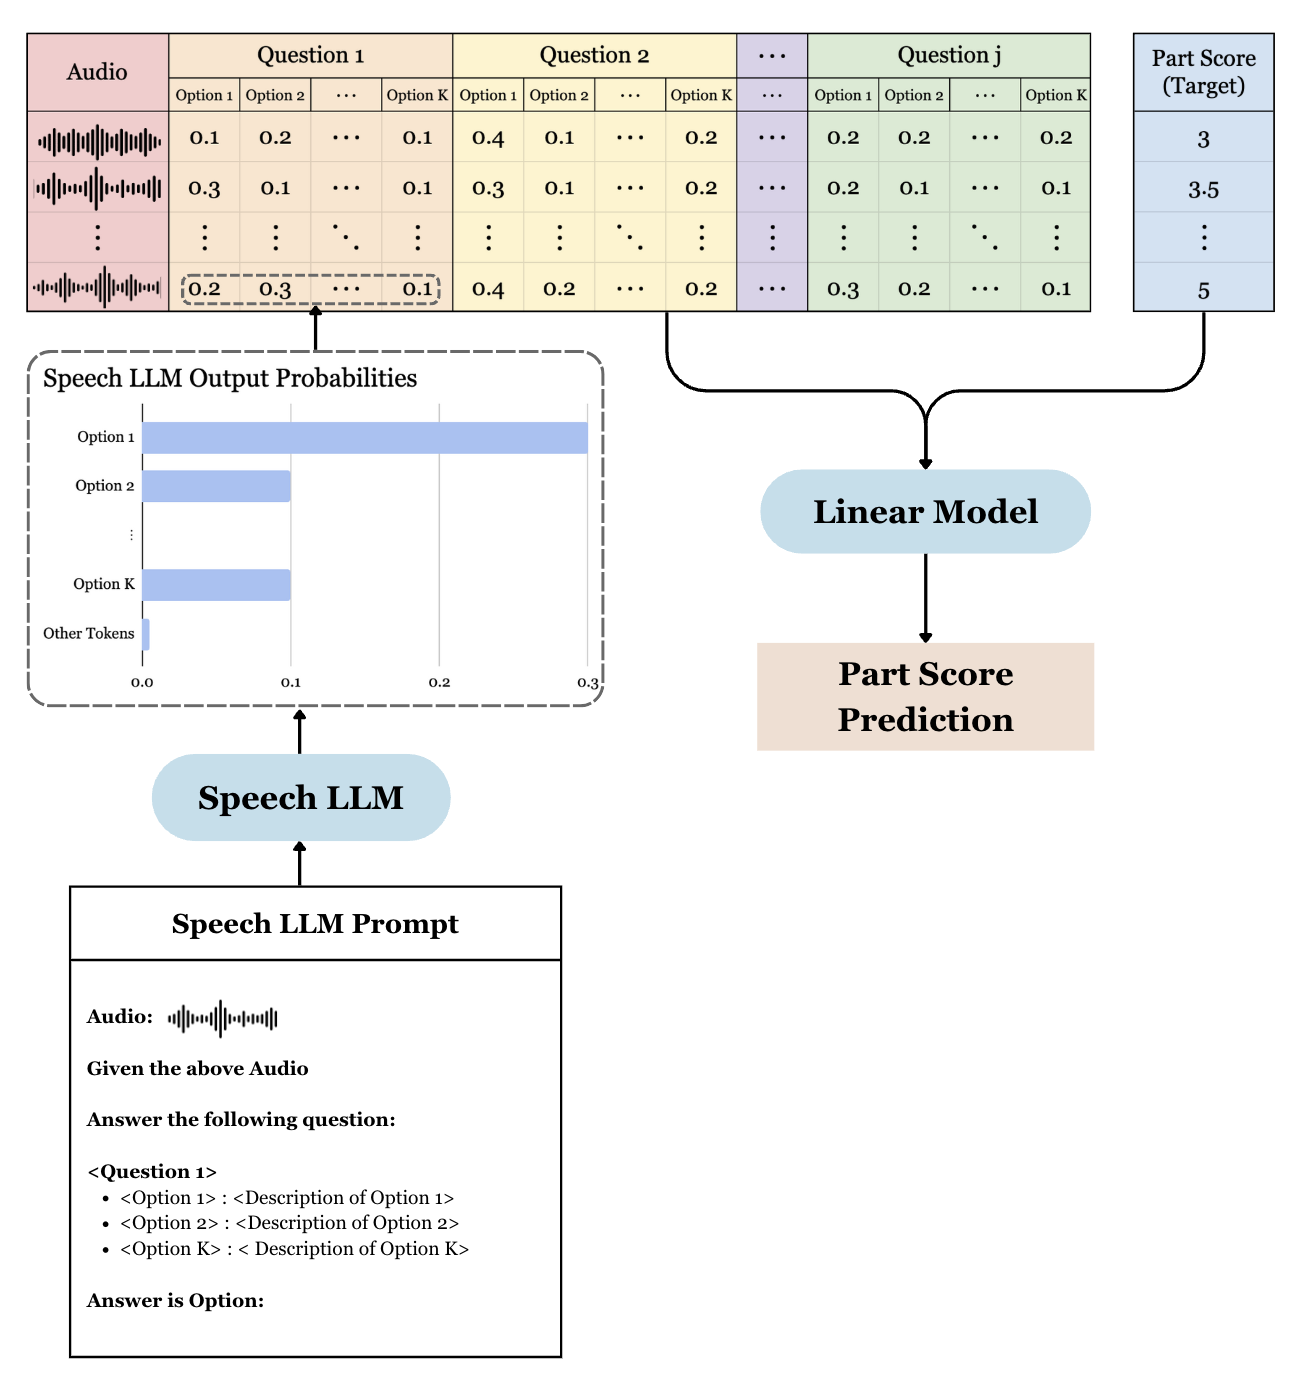
\includegraphics[width=1\linewidth]{images/overall_method_schematic.png}
  \caption{Schematic illustration of the question-based feature extraction process. The speech LLM is prompted to answer each question for every audio sample. The output probabilities for each option are collected into a table to form the interpretable feature matrix $\mathbf{Z}$, which is then used to train a regression model to predict the target variable (part scores).}
  \label{fig:question_based_approach}
\end{figure}

\subsection{Final Regression Model}
\label{subsec:final_regression_model}
With the interpretable feature matrix $\mathbf{Z}$ constructed, the final step is to predict the assessment scores. We fit a regression model to learn the mapping from our question-based feature vectors to the ground-truth scores: $f: \mathbb{R}^{M \times K} \to \mathbb{R}$. We train this regression model using the dataset $\{(\mathbf{z}_i, y_i)\}_{i=1}^N$, where $\mathbf{z}_i$ is the feature vector for audio sample $\mathbf{x}_i$ and $y_i$ is the corresponding human-assigned score.

While any regression algorithm could theoretically be applied at this stage, our empirical analysis reveals that simple linear regression achieves equivalent or superior performance to more sophisticated non-linear approaches (see Section \ref{sec:comparison_of_models}). Although the effectiveness of linear regression might initially suggest enhanced interpretability through coefficient analysis, this advantage is largely negated by the high correlation observed among the extracted features, which complicates meaningful interpretation of individual regression weights. That being said, the features themselves remain interpretable on their own which is still useful. A detailed examination of these feature correlations and their implications for interpretability is presented in Section \ref{sec:interpretable_feature_analysis}. 

Formally, we define our linear regression model as:
$$
\hat{\mathbf{y}} = \mathbf{Z}\mathbf{w} + w_0 \mathbf{1}
$$
where $\hat{\mathbf{y}} \in \mathbb{R}^N$ is the vector of predicted scores, $\mathbf{Z} \in \mathbb{R}^{N \times (M \times K)}$ is our feature matrix, $\mathbf{w} \in \mathbb{R}^{M \times K}$ is the vector of regression coefficients, $w_0 \in \mathbb{R}$ is the intercept term, and $\mathbf{1} \in \mathbb{R}^N$ is a vector of ones. To include the intercept term in matrix form, we augment our feature matrix as $\tilde{\mathbf{Z}} = [\mathbf{1}, \mathbf{Z}] \in \mathbb{R}^{N \times (M \times K + 1)}$ and define $\tilde{\mathbf{w}} = [w_0, \mathbf{w}^T]^T \in \mathbb{R}^{M \times K + 1}$, giving us $\hat{\mathbf{y}} = \tilde{\mathbf{Z}}\tilde{\mathbf{w}}$. The optimal coefficients are obtained via the normal equation:
$$
\tilde{\mathbf{w}}^* = (\tilde{\mathbf{Z}}^T\tilde{\mathbf{Z}})^{-1}\tilde{\mathbf{Z}}^T\mathbf{y}
$$
where $\mathbf{y} \in \mathbb{R}^N$ is the vector of ground-truth scores. In practice, we utilize the scikit-learn \citep{scikit-learn} \texttt{LinearRegression} implementation.

\chapter{Experiments}
\label{chap:experiments}
In this chapter, we describe our experimental setup to evaluate our proposed method. We begin by introducing the Speak \& Improve Corpus 2025 dataset used for our experiments in Section \ref{sec:dataset}. Next, we outline the baseline methods against which we compare our approach in Section \ref{sec:baselines}, including a cascaded BERT-based system and an end-to-end speech LLM representation-based system. We then detail the four specific question sets employed in our experiments in Section \ref{sec:question_sets}: the \emph{Initial Question Set}, \emph{Direct Scoring Question}, \emph{Rubric-based Question Set}, and \emph{Revised Question Set}. The complete question sets and prompts are provided in Appendix \ref{app:full_question_sets}. We discuss implementation details including our use of \textsc{Qwen2.5-Omni} and vLLM for inference in Section \ref{sec:implementation_details}. Finally, we describe the two-stage calibration procedure and five evaluation metrics (RMSE, PCC, SRC, P@0.5, P@1.0) used to assess model performance in Section \ref{chap:calibration_and_evaluation_metrics}.

\section{Dataset}
\label{sec:dataset}
We perform our experiments on the Speak \& Improve Corpus 2025 \citep{knill2024sandi}, a publicly available dataset with 315 hours of L2 English learner speech recordings with human-assigned CEFR-aligned holistic scores. The data comes from the Speak \& Improve web-app, a research project developed at the University of Cambridge, where L2 English learners from around the world practice their speaking skills by completing various speaking tasks and receiving automated feedback.

A single test consists of five parts, of which all except part 2 have been released. Part 1 is an interview where the learner is asked 8 questions about themselves. They are given 10 seconds of speaking time for the first 4 questions, and 20 seconds for the second 4. The first two questions, which may contain personal identity information, are not marked and are not included in this corpus. Part 2 consists of a read-aloud task where the learner must read aloud 8 sentences. Part 3 is a long turn task where the learner has 1 minute to give their opinion on a specific topic using 3 questions to guide them. Part 4 is another long turn task where the learner has 1 minute to describe a process depicted in a diagram. Finally, Part 5 is a communication activity where the learner has to respond to 5 questions relating to an overall topic, each for up to 20 seconds.

Each part receives a score from 1.0 (corresponding to A1 on the CEFR scale) to 6.0 (C2 on the CEFR scale) in increments of 0.5, with half scores allowed. The lowest score in the dataset is 2.0 (A2) and the highest is 5.5 (C1+), reflecting the L2 learner population. The overall test score is computed as the average of all parts except part 2, which is not included in the corpus. The dataset comes with 3 pre-defined splits: train ($\sim$3000 submissions per part), dev (438 submissions per part), and eval (442 submissions per part). Audio files are provided as 16 kHz single-channel FLAC files.

For our approach, we employ the same question set for all parts, but train individual regression models for each part separately, with the overall predicted score calculated as the mean of the predicted part scores. It is important to note that the dataset lacks analytic scores for individual assessment sub-components, meaning our method must extract interpretable features representing these sub-components in an unsupervised manner.

\section{Baselines}
\label{sec:baselines}
To evaluate the effectiveness of our question-based approach, we compare against two \emph{black-box} baseline methods: a cascaded BERT-based system and an end-to-end speech LLM representation-based system.

\subsection{BERT Baseline}
Our first baseline follows the established cascaded pipeline approach used as the baseline in the Speak \& Improve Challenge 2025 \citep{qian2024sandi}. This baseline comprises of an ASR component to convert speech-to-text and a BERT-based text grader to predict scores from the transcripts.

First, OpenAI Whisper (small) \citep{radford2022robustspeechrecognitionlargescale} is used to generate transcripts from the audio recordings. These transcriptions are normalised by removing punctuation and converting to lowercase. Next, a BERT-based grader is finetuned to predict scores from the transcripts. These graders consist of a BERT-base-uncased \citep{devlin2019bertpretrainingdeepbidirectional} text encoder followed by four multi-head self-attention layers whose outputs are concatenated and passed through two fully connected layers before finally mapping to a single scalar output. The weights for the encoder of the BERT-based grader are initialised from BERT-base-uncased, and a separate BERT-based grader is finetuned for each test part (Parts 1, 3, 4, and 5). The final submission-level score is computed as the average of the per-part predicted scores. We will refer to this baseline as the \emph{BERT Baseline} throughout the rest of this dissertation. Further details regarding this baseline can be found in \citet{qian2024sandi}.

\subsection{Speech LLM Representations}
Our second baseline utilizes the multimodal capabilities of speech LLMs for direct end-to-end scoring. We prompt \textsc{Qwen2.5-Omni} \citep{xu2025qwen25omnitechnicalreport} to predict scores directly from audio inputs and extract the final layer hidden state representation corresponding to the predicted options token. This hidden state, with $3584$ dimensions, is conditioned on the task prompt and the audio input, allowing it to capture rich semantic and acoustic information relevant to the scoring task. A regression model is then trained on these representations to predict final scores. Given that the feature dimensionality ($3584$) exceeds the available training samples per test part, we employ ridge regression rather than ordinary least squares to address the resulting rank deficiency of the Gram matrix. Following the same structure as the BERT baseline and our proposed approach, we train separate models for each test part and compute the final submission-level score by averaging the predicted part scores.

This baseline slightly differs from the regression approach used in \citet{ma2025assessment}, who fine-tune LoRA adaptors along with a final linear layer. However, our approach of training a regression model on fixed final layer representations is computationally cheaper and performs comparably well in practice (see Section \ref{sec:comparison_of_models} and \citet{ma2025assessment}). Therefore, this baseline is near state-of-the-art making it significantly challenging to outperform. However, unlike our question-based approach, this method does not provide any interpretable features or insights into the scoring process. We refer to this baseline as the \emph{Speech LLM Representations} throughout the rest of this dissertation.

\section{Question Sets}
\label{sec:question_sets}
Our experiments evaluate four distinct question sets: \emph{Initial Question Set}, \emph{Direct Scoring Question}, \emph{Rubric-based Question Set}, and \emph{Revised Question Set}. These question sets differ in the number of questions, the number of options per question, and their design methodology. Table \ref{table:question_sets} summarizes the key characteristics of each question set. 

\begin{table}[h]
\centering
\begin{tabular}{|l|c|c|l|}
\hline
\textbf{Question Set} & \textbf{Questions} & \textbf{Options} & \textbf{Design Methodology} \\
\hline
\emph{Initial Question Set} & 14 & ``High'', ``Medium'', ``Low'' & LLM generated \\
\hline
\emph{Direct Scoring Question} & 1 & ``A'', ``B'', ``C'', ``D'', ``E'', ``F'' & One question \\
\hline
\emph{Rubric-based Question Set} & 3 & ``A'', ``B'', ``C'', ``D'', ``E'', ``F'' & Rubric based \\
\hline
\emph{Revised Question Set} & 30 & ``High'', ``Low'' & Expert enhanced \\
\hline
\end{tabular}
\caption{Overview of question sets used in experiments.}
\label{table:question_sets}
\end{table}

The \emph{Initial Question Set} consists of 14 questions generated using ChatGPT o3. The LLM was prompted with the Linguaskill Speaking Global Assessment Criteria rubric \citep{cambridge2020linguaskill} and instructed to generate questions that would be both necessary and sufficient for determining final scores. Following the TRATES methodology \citep{eltanbouly2025tratestraitspecificrubricassistedcrossprompt}, each question has three options: ``High'', ``Medium'', and ``Low''. The complete question set is provided in Section~\ref{app_sec:initial_question_set} in Appendix~\ref{app:full_question_sets}.

The \emph{Direct Scoring Question} exists within a question set with a single question that asks the speech LLM to predict the final score directly. The speech LLM is presented with the Linguaskill Speaking Global Assessment Criteria rubric \citep{cambridge2020linguaskill} verbatim (with options A1 to C2 mapped to F to A) and asked to select a single option representing the final score across all three dimensions of the rubric (Pronunciation and Fluency, Language Resource, and Discourse Management). The goal of this question set is to assess the value of having multiple questions versus a single direct scoring question. The prompt used for this question is shown in Section~\ref{app_sec:direct_scoring_prompt} in Appendix~\ref{app:full_question_sets}.

The \emph{Rubric-based Question Set} consists of three questions, each corresponding to one of the three criteria in the Linguaskill Speaking Global Assessment Criteria rubric \citep{cambridge2020linguaskill}. Each question has six options (A, B, C, D, E, F) corresponding to the six levels in the rubric. This question set is designed to directly reflect the rubric structure while still decomposing the scoring task into multiple dimensions. The advantage of this approach is that it ensures tight alignment between the extracted interpretable features and the rubric criteria. The complete \emph{Rubric-based Question Set} is provided in Section~\ref{app_sec:rubric_based_question_set} in Appendix~\ref{app:full_question_sets}.

The \emph{Revised Question Set} is a more comprehensive version of the \emph{Initial Question Set}, expanded to 30 questions that incorporate feedback from subject matter experts—specifically, experienced oral assessment graders who regularly evaluate spoken language proficiency. Starting from the initial 14 questions, these experts modified existing questions and contributed additional ones based on their practical grading experience, resulting in a comprehensive set of 30 questions. Notably, this question set also contains generic questions about the audio quality (e.g., background noise, volume) to help the model account for extraneous factors that may affect intelligibility. A key modification in this question set is the reduction from three response options to two: ``High'' and ``Low''. The Medium option was deliberately removed to encourage the speech LLM to make more decisive judgements rather than defaulting to neutral responses. This binary choice format forces the model to ``pick a side'' for each assessed trait, potentially leading to more discriminative features while also reducing the dimensionality of the feature space. The complete \emph{Revised Question Set} is provided in Section~\ref{app_sec:revised_question_set} in Appendix~\ref{app:full_question_sets}.

\section{Implementation Details}
\label{sec:implementation_details}
Our implementation leverages vLLM \citep{kwon2023efficientmemorymanagementlarge} for speech LLM inference, providing high-throughput serving with optimized memory management through PagedAttention. The system uses a generic system prompt: \emph{``You are a helpful assistant."} for simplicity. Note that typical generation parameters such as temperature, top-k, and top-p are irrelevant for our methodology, as we only extract the probability distribution over the vocabulary for the immediate next token following the prompt, rather than performing autoregressive text generation.

Given the Speak \& Improve datasets restrictions prohibiting the use of model APIs and requiring only self-hosted open-source models \citep{knill2024sandi}, we deployed the 7B parameter Qwen2.5-Omni model on cloud GPU infrastructure using vLLM. This self-hosting approach presented significant engineering challenges, including configuring audio-specific tokenization schemes, managing multi-modal data processors, and handling audio encoding requirements that distinguish speech LLMs from standard text-based models.

A crucial optimization involves consecutive inference on the same audio sample to preserve the common key-value (KV) cache. When processing multiple questions for a single audio recording, all questions for that sample are processed sequentially before moving to the next audio file. This allows the model to maintain the computationally expensive audio representation in its KV cache across questions, dramatically reducing inference overhead compared to re-encoding the audio for each question. The scale of inference required was substantial, with approximately 48,000 audio files processed for each experiment experiment, and the multi-question approach multiplying the total number of inference calls by the number of questions in each set. To address I/O bottlenecks arising from reading audio files, we implemented batching strategies that process audio files in groups of 10,000 before passing them to vLLM, optimizing throughput by ensuring vLLM has sufficient data for its internal batching mechanisms.

For embedding extraction, we utilized Hugging Face's \texttt{transformers} library \citep{wolf2020huggingfacestransformersstateoftheartnatural} and adopted the Apache Parquet file format \citep{apache_parquet} for efficient storage and retrieval of the embedding data generated throughout our experiments.

In our experiments, we explore two strategies for posing questions to the speech LLM: sequential question inference and batch question inference. With \textbf{sequential question inference}, each question is posed to the speech LLM in separate inference calls. For a question-set with $M$ questions, this requires $M$ distinct inference requests. This allows the model to focus exclusively on one assessment dimension at a time, potentially leading to more focused and accurate evaluations. The prompt used for sequential inference is shown in Figure \ref{fig:sequential_inference_prompt}.

\begin{figure}[h]
  \centering
  \begin{tcolorbox}[
    colback=white,
    colframe=black,
    boxrule=0.8pt,
    arc=4pt,
    width=0.95\linewidth,
    sharp corners=south,
    title=Sequential Inference Prompt Template
  ]
    \small
    You are an examiner grading a spoken English test for non-native (L2) speakers.

    You will be given an audio file of a candidate's speech, and you must answer the following question based on the audio content.

    \textbf{Question:} \{question\}

    \textbf{Options:} \{options\}

    Please select \textbf{ONLY one} of the options (\{option\_keys\}) that best describes the candidate's performance. Respond with the option only.

    \textbf{Answer:}
  \end{tcolorbox}
  \caption{Prompt template used for sequential question inference with the speech LLM.}
  \label{fig:sequential_inference_prompt}
\end{figure}

With \textbf{batch question inference}, all questions are presented simultaneously in a single inference call, with the speech LLM producing a structured JSON response containing scores for all criteria. This strategy significantly reduces computational costs by requiring only one inference call per audio sample. However, the simultaneous consideration of multiple assessment criteria may lead to cognitive overload \citep{cheng2023batchpromptingefficientinference}, where the model struggles to maintain equal attention across all questions.

For the \emph{Rubric-based Question Set} and the \emph{Revised Question Set}, we evaluate both inference strategies to assess their impact on performance. The prompts used for batch inference are shown in Section~\ref{app_sec:rubric_based_question_set_batch} and Section~\ref{app_sec:revised_question_set_batch} in Appendix~\ref{app:full_question_sets}.

\section{Calibration and Evaluation Metrics}
\label{chap:calibration_and_evaluation_metrics}
Due to the distribution of scores in the dataset being dense in the middle and sparse at the extremes, any fitted model tends to heavily regress towards the mean. Following standard practice in the field \citep{qian2024sandi,ma2025assessment}, we compute calibration parameters to correct for this effect.

The calibration procedure consists of two stages, as illustrated in Figure \ref{fig:calibration_procedure}. First, for each assessment part, we fit a linear transformation to predict the ground-truth part scores from the predicted part scores on the dev set. This linear transformation is then applied to all predicted part scores. The predicted overall score is computed as the average of these calibrated predicted part scores. Second, an additional linear calibration is applied to the predicted overall score by fitting a linear transformation on the dev set to predict the ground-truth overall scores from the predicted overall scores (which are themselves the average of the calibrated part scores). This two-stage calibration procedure represents standard practice in the field \citep{qian2024sandi, ma2025assessment} and is necessary to ensure that predicted scores are well-aligned with ground-truth scores. This calibration procedure is applied consistently to all models, including the baselines, to ensure fair comparison.

\begin{figure}[h]
  \centering
  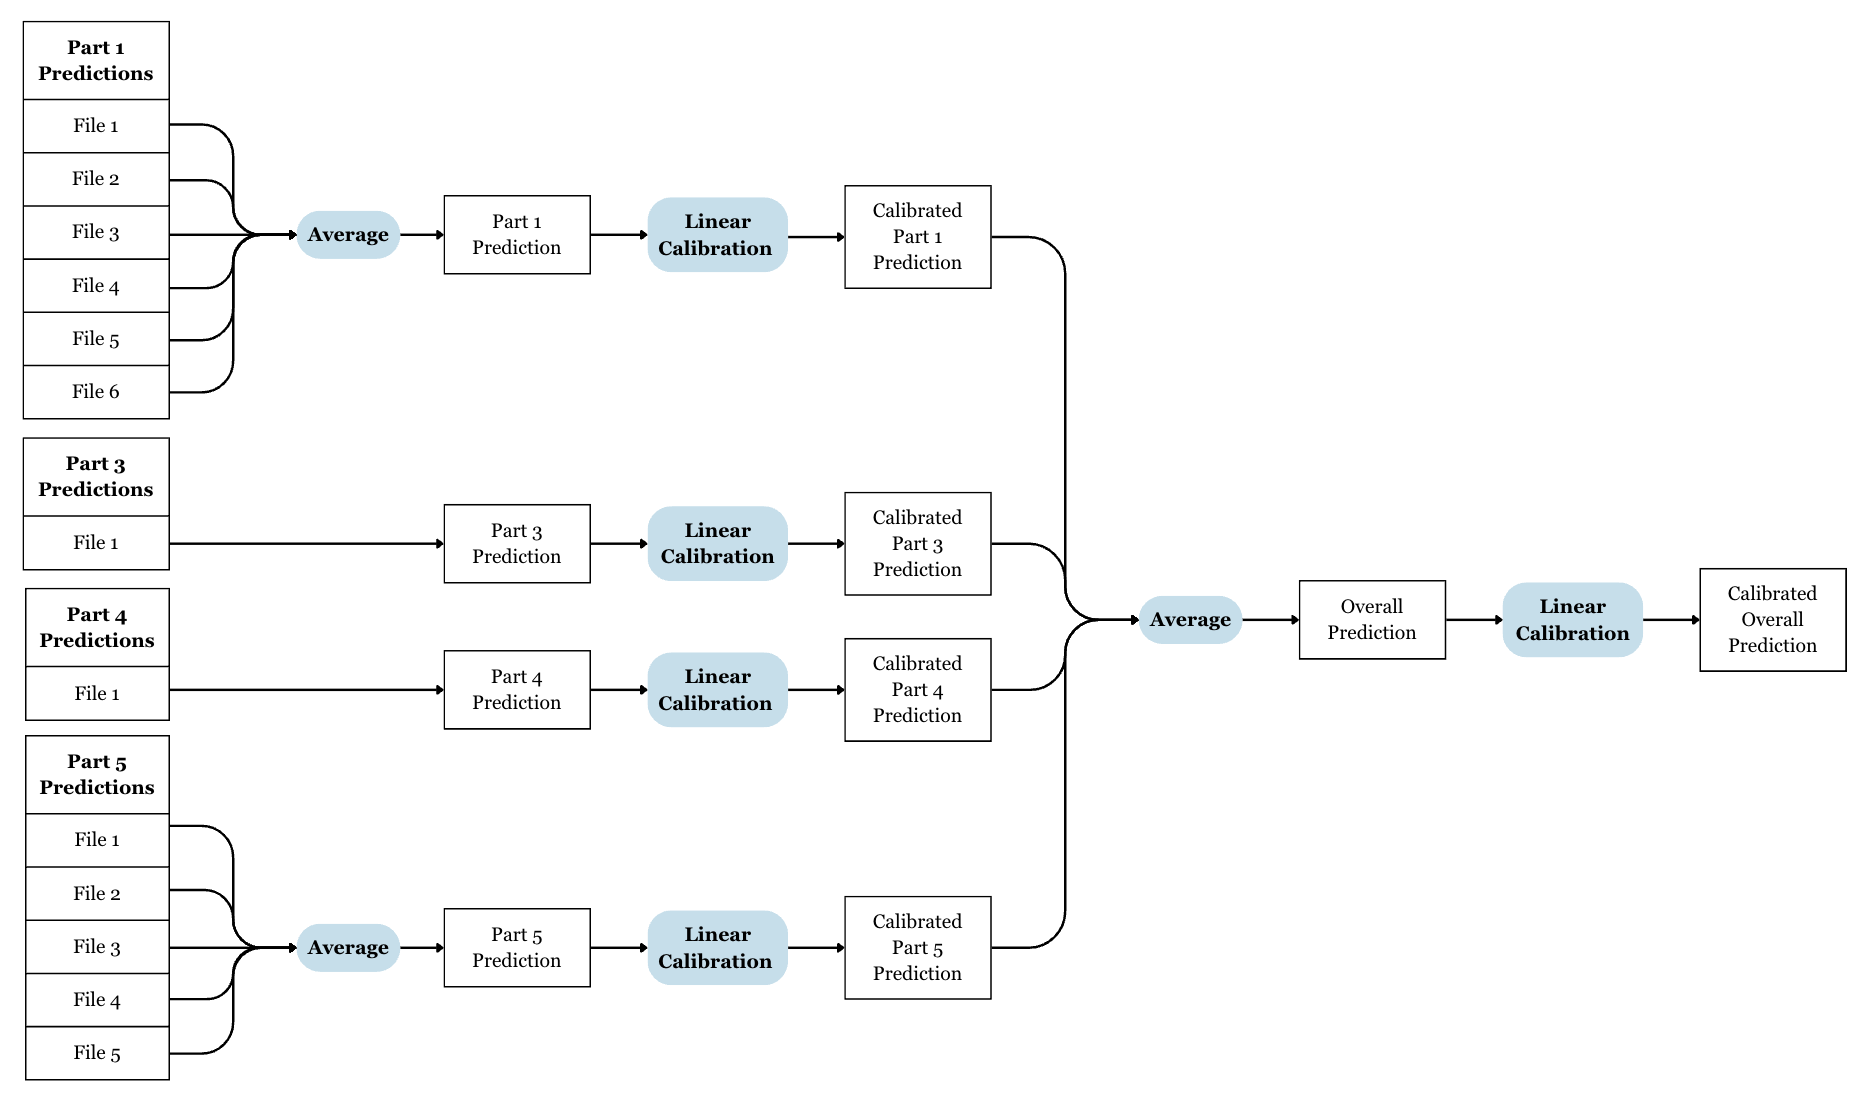
\includegraphics[width=1\linewidth]{images/calibration_schematic.png}
  \caption{Illustration of the two-stage calibration procedure used to align predicted scores with ground-truth scores. First, predictions from all files of a given speaker are averaged to obtain speaker-level scores (this is relevant for parts 1 and 5 where multiple files exist per speaker). Next, a linear calibration is applied to each part's predicted scores. The overall predicted score is computed as the average of the calibrated part scores, followed by a second linear calibration to align with ground-truth overall scores. Note that each linear calibration has its own slope and intercept parameters that are fitted on the dev set.}
  \label{fig:calibration_procedure}
\end{figure}

For evaluation, we employ five standard metrics commonly used in spoken language assessment. Root Mean Square Error (RMSE) measures the average magnitude of prediction errors, with lower values indicating better performance. Pearson Correlation Coefficient (PCC) quantifies the linear relationship between predicted and ground-truth scores, ranging from -1 to 1, where values closer to 1 indicate stronger positive correlation. Spearman Rank Correlation (SRC) is essentially PCC applied to the ranks of the data rather than the raw values. It assesses the monotonic relationship between predictions and true scores, providing insight into how well the model preserves the relative ordering of submissions. Precision at 0.5 (P@0.5) represents the percentage of predictions within 0.5 points of the ground truth, while Precision at 1.0 (P@1.0) indicates the percentage within 1.0 point. Both precision metrics serve as measures of practical accuracy for educational assessment applications. It is important to note that the calibration procedure does not affect PCC or SRC, as these correlation metrics are invariant to linear transformations of the predictions.

\chapter{Results and Discussion}
\label{chap:results_discussion}
In this chapter, we present and discuss the results from various experiments with our proposed question-based approach. We begin by comparing different feature transformations in Section \ref{sec:comparison_of_transformations}, followed by an evaluation of different regression models in Section \ref{sec:comparison_of_models}. We then analyze the impact of different question sets on performance in Section \ref{sec:comparison_of_feature_sets} and provide visual inspection of these results in Section \ref{sec:visual_inspection}. Next, we analyze and discuss the interpretability of the extracted features in Section \ref{sec:interpretable_feature_analysis}. Finally, we investigate the scalability of our approach in low data regimes in Section \ref{sec:low_data_regime}.

For consistency with the Speak \& Improve Challenge 2025 \citep{qian2024sandi} and \citet{ma2025assessment}, all results reported in this chapter are evaluated on the dev set unless otherwise specified. 
Hyperparameters for all models were tuned using cross-validation on the training set, ensuring the dev set remained completely unseen during model development. Calibration parameters, as described in Section~\ref{chap:calibration_and_evaluation_metrics}, were still computed on the dev set following standard practice.
Results are reported as overall submission-level scores, computed as the average of predicted part scores across test components. All metrics are presented as mean $\pm$ standard deviation over 1000 bootstrapped samples of the data.

\section{Comparison of Transformations}
\label{sec:comparison_of_transformations}
In this section, we compare different transformations of the speech LLM outputs to construct the feature matrix. We evaluate four different feature transformations of the \emph{Initial Question Set} features to understand how the representation of the speech LLMs responses affects downstream performance. The \textbf{original feature matrix} (represented as ``Original'' in table \ref{table:feature_transformations}) contains the raw log-probabilities of each option as output by the speech LLM. The \textbf{discrete feature matrix} (represented as ``Discrete'' in table \ref{table:feature_transformations}) contains one-hot encoded representations of the selected option for each question (i.e., the argmax of the log-probabilities), effectively converting the continuous probability distribution into a categorical choice. The \textbf{exponentiated feature matrix} (represented as ``Exp.'' in table \ref{table:feature_transformations}) contains the exponentiated log-probabilities, which correspond to the actual probabilities of each option. Finally, the \textbf{softmax feature matrix} (represented as ``Softmax'' in table \ref{table:feature_transformations}) contains the softmax-normalised probabilities of each option, ensuring that the probabilities for each question sum to 1, unlike the exponentiated feature matrix where probabilities may sum to less than 1 due to the non-zero probabilities assigned to invalid tokens.

The results are shown in Table \ref{table:feature_transformations}. Several key observations emerge from this comparison. First, the discrete feature matrix performs significantly worse than all continuous representations, indicating that the richer information contained in the probability distributions is crucial for performance. These findings can be explained by two theories: (1) the log-probabilities capture the model's uncertainty about each option, which provides valuable information for the regression model, and (2) the continuous probabilities help overcome the LLMs' positional bias \citep{liusie2023mitigatingwordbiaszeroshot} of selecting the same options regardless of the question or audio content. Among the continuous representations, the exponentiated feature matrix performs best, followed closely by the original log-probability feature matrix, and then the softmax-normalised feature matrix. The poorer performance of the softmax-normalised features may be attributed to the fact that normalising only across valid options discards probability mass assigned to other tokens in the vocabulary, potentially reducing signal if the model's certainty over the full vocabulary is meaningful for assessment.

\begin{table}[h]
\centering
\resizebox{\linewidth}{!}{
\begin{tabular}{|l|c|c|c|c|c|}
\hline
\textbf{Feature Transformation} & \textbf{RMSE} & \textbf{PCC} & \textbf{SRC} & \textbf{P@0.5} & \textbf{P@1.0} \\
\hline
Original Features (logprobs) & 0.4278 $\pm$ 0.0086 & 0.7529 $\pm$ 0.0111 & 0.7525 $\pm$ 0.0121 & 77.67 $\pm$ 1.01 & 97.62 $\pm$ 0.35 \\
Discrete Features & 0.4964 $\pm$ 0.0097 & 0.6628 $\pm$ 0.0140 & 0.6661 $\pm$ 0.0148 & 69.94 $\pm$ 1.11 & 95.56 $\pm$ 0.48 \\
Exponentiated Features (probs) & \textbf{0.4200 $\pm$ 0.0081} & \textbf{0.7640 $\pm$ 0.0103} & \textbf{0.7630 $\pm$ 0.0116} & \textbf{78.75 $\pm$ 1.00} & \textbf{97.75 $\pm$ 0.35} \\
Softmax Normalized Features (probs) & 0.4401 $\pm$ 0.0088 & 0.7355 $\pm$ 0.0116 & 0.7390 $\pm$ 0.0125 & 76.33 $\pm$ 1.04 & 97.52 $\pm$ 0.37 \\
\hline
\end{tabular}
}
\caption{Performance comparison of linear models using different feature transformations applied to the \emph{Initial Question Set}.}
\label{table:feature_transformations}
\end{table}

\section{Comparison of Models}
\label{sec:comparison_of_models}
After establishing the best feature transformation, we compare different regression models trained on the exponentiated feature matrix from the \emph{Initial Question Set}. Specifically, we compare linear regression, ridge regression, elastic net regression, KNN regression with various distance metrics (euclidean, manhattan), support vector regression (SVR) with linear and RBF kernels, XGBoost regression, and multi-layer perceptron regression networks. We performed comprehensive hyperparameter tuning for each model using cross-validation on the training set to ensure optimal performance. The results are shown in Table \ref{table:regression_models}. The results indicate that linear regression performs comparably to all other models, indicating that the relationship between the extracted features and the final scores is largely linear.

\begin{table}[h]
\centering
\resizebox{\linewidth}{!}{
\begin{tabular}{|l|c|c|c|c|c|}
\hline
\textbf{Model} & \textbf{RMSE} & \textbf{PCC} & \textbf{SRC} & \textbf{P@0.5} & \textbf{P@1.0} \\
\hline
Linear Regression & 0.3945 $\pm$ 0.0150 & 0.8052 $\pm$ 0.0153 & 0.8150 $\pm$ 0.0165 & 81.76 $\pm$ 1.82 & \textbf{97.46 $\pm$ 0.74} \\
Ridge Regression & 0.3944 $\pm$ 0.0150 & 0.8053 $\pm$ 0.0153 & 0.8153 $\pm$ 0.0165 & \textbf{81.99 $\pm$ 1.82} & \textbf{97.46 $\pm$ 0.74} \\
ElasticNet Regression & \textbf{0.3942 $\pm$ 0.0150} & \textbf{0.8055 $\pm$ 0.0153} & 0.8155 $\pm$ 0.0165 & 81.76 $\pm$ 1.83 & \textbf{97.46 $\pm$ 0.74} \\
KNN Regression & 0.4180 $\pm$ 0.0162 & 0.7779 $\pm$ 0.0176 & 0.7878 $\pm$ 0.0187 & 79.43 $\pm$ 1.99 & 96.77 $\pm$ 0.83 \\
Support Vector Regression & 0.3944 $\pm$ 0.0151 & 0.8053 $\pm$ 0.0153 & \textbf{0.8163 $\pm$ 0.0163} & 81.73 $\pm$ 1.87 & \textbf{97.46 $\pm$ 0.74} \\
XGBoost Regression & 0.4068 $\pm$ 0.0158 & 0.7911 $\pm$ 0.0167 & 0.8009 $\pm$ 0.0178 & 80.63 $\pm$ 1.87 & 97.24 $\pm$ 0.77 \\
MLP Regression & 0.4049 $\pm$ 0.0161 & 0.7934 $\pm$ 0.0166 & 0.8103 $\pm$ 0.0165 & 79.90 $\pm$ 1.96 & \textbf{97.46 $\pm$ 0.73} \\
\hline
\end{tabular}
}
\caption{Performance comparison of various regression models using features from the \emph{Initial Question Set}.}
\label{table:regression_models}
\end{table}

\section{Comparison of Feature Sets}
\label{sec:comparison_of_feature_sets}
We now compare the performance of linear models trained on exponentiated feature matrices across different question sets. As detailed in Section \ref{sec:question_sets}, we evaluate four distinct question sets: the \emph{Initial Question Set} with 14 questions using ``High''/``Medium''/``Low'' options, the \emph{Direct Scoring Question} with 1 question using 6 CEFR levels, the \emph{Rubric-based Question Set} with 3 questions using 6 CEFR levels, and the \emph{Revised Question Set} with 30 questions using ``High''/``Low'' options. For the rubric-based and revised question sets, we compare both individual inference where each question is posed separately and batch inference where all questions are presented simultaneously in a single prompt, as described in Section \ref{sec:implementation_details}.

Our comparison also includes two baseline methods: the \emph{BERT Baseline}, which uses Whisper ASR followed by a BERT text grader, and the \emph{Speech LLM Representations}, which extracts 3584-dimensional hidden state representations from the final layer of Qwen2.5-Omni conditioned on a direct scoring prompt, as detailed in Section \ref{sec:baselines}.

To further analyze our approach, we evaluate a \emph{Combined Question Set} that concatenates features from all individual question sets (including both batch and individual inference where applicable). Additionally, we implement random projections of the \emph{Initial Question Set} to match the dimensionality of the \emph{Combined Question Set} (204). This involves multiplying the initial 42-dimensional feature vector by a random matrix $\mathbf{R} \in \mathbb{R}^{42 \times 204}$ where each entry is drawn from a uniform distribution over $[0, 1]$, allowing us to assess whether performance gains are simply due to higher dimensionality enabling the linear model to capture more complex relationships, or if the specific information contained in different question sets is beneficial.

Finally, we concatenate the \emph{Combined Question Set} features with the speech LLM representations to determine whether our question-based approach provides complementary information beyond the black-box speech LLM features. The model trained on this feature set uses ridge regression, consistent with the \emph{Speech LLM Representations}, to handle the high-dimensional feature space (204 combined question features plus 3584 speech LLM features).

\begin{table}[h]
\centering
\resizebox{\linewidth}{!}{
\begin{tabular}{|l|c|c|c|c|c|}
\hline
\textbf{Feature Set} & \textbf{RMSE} & \textbf{PCC} & \textbf{SRC} & \textbf{P@0.5} & \textbf{P@1.0} \\
\hline
\emph{BERT Baseline} & 0.445 & 0.746 & 0.750 & 73.3 & 96.6 \\
\emph{Initial Question Set} & 0.3945 $\pm$ 0.0150 & 0.8052 $\pm$ 0.0153 & 0.8150 $\pm$ 0.0165 & 81.76 $\pm$ 1.82 & 97.46 $\pm$ 0.74 \\
\emph{Direct Scoring Question} & 0.4454 $\pm$ 0.0171 & 0.7427 $\pm$ 0.0206 & 0.7484 $\pm$ 0.0220 & 75.35 $\pm$ 2.14 & 96.76 $\pm$ 0.84 \\
\emph{Rubric-based Question Set} & 0.4203 $\pm$ 0.0151 & 0.7751 $\pm$ 0.0170 & 0.7847 $\pm$ 0.0186 & 79.46 $\pm$ 1.92 & 97.26 $\pm$ 0.78 \\
\emph{Rubric-based Question Set} (Batch Inference) & 0.4247 $\pm$ 0.0165 & 0.7696 $\pm$ 0.0185 & 0.7717 $\pm$ 0.0204 & 78.59 $\pm$ 2.02 & 96.55 $\pm$ 0.87 \\
\emph{Revised Question Set} & 0.4163 $\pm$ 0.0168 & 0.7799 $\pm$ 0.0183 & 0.7905 $\pm$ 0.0184 & 78.94 $\pm$ 1.95 & 97.48 $\pm$ 0.73 \\
\emph{Revised Question Set} (Batch Inference) & 0.4188 $\pm$ 0.0156 & 0.7769 $\pm$ 0.0176 & 0.7868 $\pm$ 0.0186 & 79.95 $\pm$ 1.87 & 97.24 $\pm$ 0.77 \\
\emph{Combined Question Set} & 0.3872 $\pm$ 0.0153 & 0.8132 $\pm$ 0.0151 & 0.8245 $\pm$ 0.0153 & 82.87 $\pm$ 1.83 & 97.93 $\pm$ 0.67 \\
Random Projections of \emph{Initial Question Set} & 0.3945 $\pm$ 0.0150 & 0.8052 $\pm$ 0.0153 & 0.8150 $\pm$ 0.0165 & 81.76 $\pm$ 1.82 & 97.46 $\pm$ 0.74 \\
\emph{Speech LLM Representations} & \textbf{0.3727 $\pm$ 0.0146} & \textbf{0.8282 $\pm$ 0.0144} & \textbf{0.8397 $\pm$ 0.0144} & 85.84 $\pm$ 1.73 & \textbf{98.17 $\pm$ 0.65} \\
\emph{Combined Question Set} + \emph{Speech LLM Representations} & \textbf{0.3727 $\pm$ 0.0147} & \textbf{0.8282 $\pm$ 0.0146} & 0.8378 $\pm$ 0.0148 & \textbf{86.28 $\pm$ 1.68} & \textbf{98.17 $\pm$ 0.65} \\
\hline
\end{tabular}
}
\caption{Performance comparison of linear regression models across different feature representations (evaluated on dev set for overall scores).}
\label{table:feature_sets}
\end{table}

The results are presented in Table \ref{table:feature_sets}. Additional results for individual parts of the overall assessment and eval set performance are provided in Appendix~\ref{app:additional_results}. Several key insights emerge from this comparison:

\textbf{BERT Baseline:} The cascaded \emph{BERT Baseline} achieves an RMSE of $0.445$ and PCC of $0.746$, which is significantly worse than all our question-based approaches, despite having far more features (768 dimensions from BERT). This indicates that our interpretable question-based features are able capture more relevant information for scoring than the text-based black-box features extracted by BERT from ASR transcripts.

\textbf{Question Set Complexity and Performance:} There is a general trend showing that more comprehensive question sets lead to better performance. The \emph{Direct Scoring Question}, using only a single question, achieves the weakest performance with an RMSE of $0.4454 \pm 0.0171$ and PCC of $0.7427 \pm 0.0206$. The \emph{Rubric-based Question Set} ($3$ questions) improves substantially to an RMSE of $0.4203 \pm 0.0151$ and PCC of $0.7751 \pm 0.0170$, while the \emph{Initial Question Set} ($14$ questions) performs even better with an RMSE of $0.3945 \pm 0.0150$ and PCC of $0.8052 \pm 0.0153$. However, this trend has a notable exception: the \emph{Revised Question Set} ($30$ questions) slightly underperforms the \emph{Initial Question Set} (RMSE of $0.4163 \pm 0.0168$ vs $0.3945 \pm 0.0150$), likely due to the reduction from three response options (``High''/``Medium''/``Low'') to two (``High''/``Low''), which indicates that the granularity of response options is also a critical factor in capturing predictive information.

\textbf{Inference Strategy Effects:} Batch inference only slightly underperforms individual inference across both question sets tested. For the \emph{Rubric-based Question Set}, batch inference shows an RMSE increase of 0.0044 and PCC decrease of 0.0055 compared to individual inference. For the \emph{Revised Question Set}, batch inference results in an RMSE increase of 0.0025 and PCC decrease of 0.0030. This performance drop is relatively small especially considering the standard deviations derived from bootstrapping, suggesting that batch inference may be a viable option when computational efficiency is a priority.

\textbf{Combining Question Sets:} The \emph{Combined Question Set}, which concatenates features from all individual question sets, achieves dramatically superior performance with an RMSE of $0.3872 \pm 0.0153$ and PCC of $0.8132 \pm 0.0151$, which is substantially better than any individual question set. Crucially, the random projection experiment maintains identical performance to the initial question set, demonstrating that the performance gains from combining question sets are not merely due to increased dimensionality. Instead, this finding indicates that different question sets capture complementary information about speaking proficiency, further supporting the general trend that more questions lead to better performance.

\textbf{Speech LLM Representations:} The \emph{Speech LLM Representations} achieve near state-of-the-art performance with a RMSE of $0.3727 \pm 0.0146$ and PCC of $0.8282 \pm 0.0144$. None of our interpretable feature sets managed to surpass this performance. This finding suggests that our question-based method essentially queries different aspects of the same underlying audio representation rather than extracting fundamentally new information. One way to conceptualize this is that each question provides a different semantic and conceptually meaningful ``view'' of the same underlying audio representation that can be interpreted more naturally than the black-box representation itself. Furthermore, the fact that combining question-based features with speech LLM representations yields no significant improvements (RMSE of $0.3727 \pm 0.0147$ vs $0.3727 \pm 0.0146$) supports this hypothesis, indicating that the question-based features do not provide substantial complementary information beyond what is already captured by the speech LLMs embeddings.

Overall, this reflects the fundamental trade-off in machine learning between interpretability and predictive accuracy. Our question-based approach achieves competitive performance with dramatically fewer features, ranging from 6 to 60, compared to the $3584$-dimensional speech LLM representations. More importantly, each of these features corresponds to a human-interpretable assessment criterion with clear conceptual meaning, enabling educators and learners to potentially understand which aspects of speaking proficiency contribute to the final score.

\section{Visual Inspection}
\label{sec:visual_inspection}
To better understand the comparative behaviour of our different feature sets, we provide a visual analysis of predictions versus ground truth scores.

Figure \ref{fig:predictions_vs_ground_truth_original} shows the predictions from the \emph{Initial Question Set} model versus ground truth scores. As with most predictive models, the regression line has a slope less than 1, reflecting the expected regression to the mean phenomenon \citep{galton_1886_1449548}, which is particularly pronounced given the datasets score distribution with most samples in the middle range (3.0–4.0) and sparse tails.

\begin{figure}[h]
  \centering
  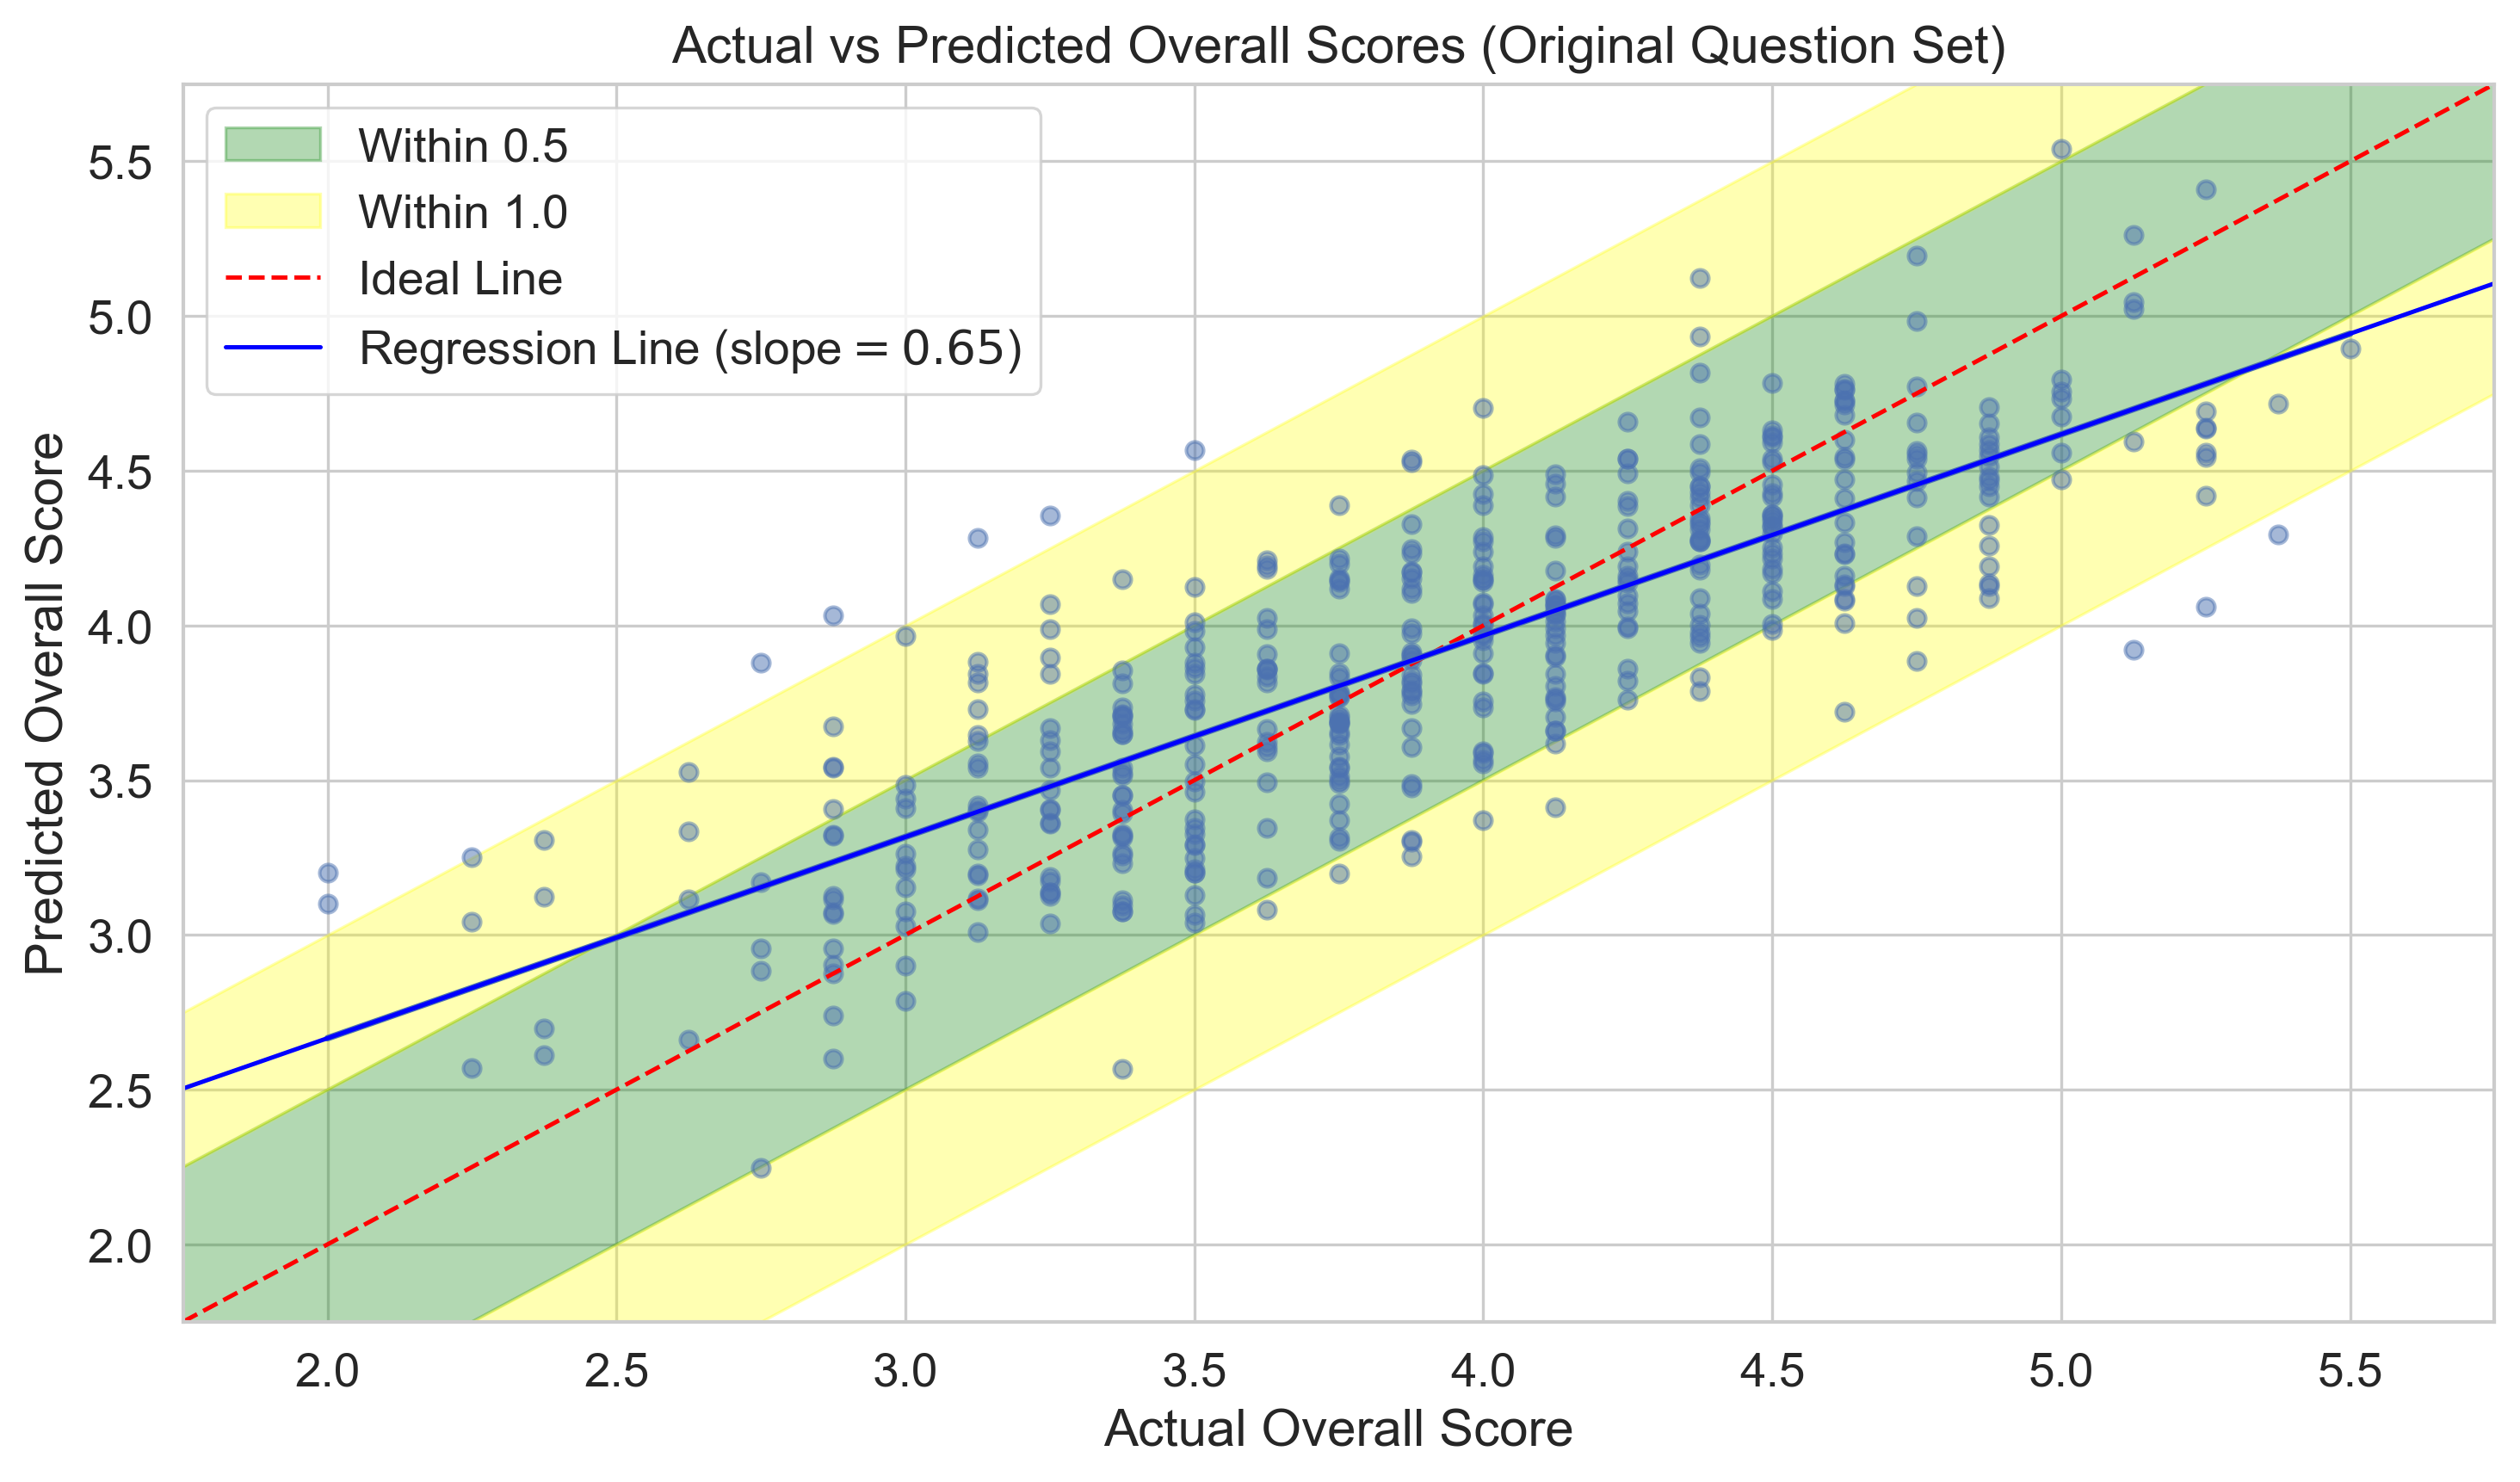
\includegraphics[width=1\linewidth]{images/actual_vs_predicted_orig.png}
  \caption{Predictions versus ground truth scores for the \emph{Initial Question Set}. The diagonal line represents perfect predictions, while the fitted line shows the actual model behaviour.}
  \label{fig:predictions_vs_ground_truth_original}
\end{figure}

More importantly, comparing across all feature sets in Figure \ref{fig:predictions_vs_ground_truth_all} reveals differences in how well different feature representations capture the full range of scores. Feature sets with higher predictive performance (higher PCC) demonstrate slopes closer to 1 and better capture extreme values, with the \emph{Speech LLM Representations} showing the steepest slope, followed by the \emph{Combined Question Set}, and then individual question sets.

\begin{figure}[h]
  \centering
  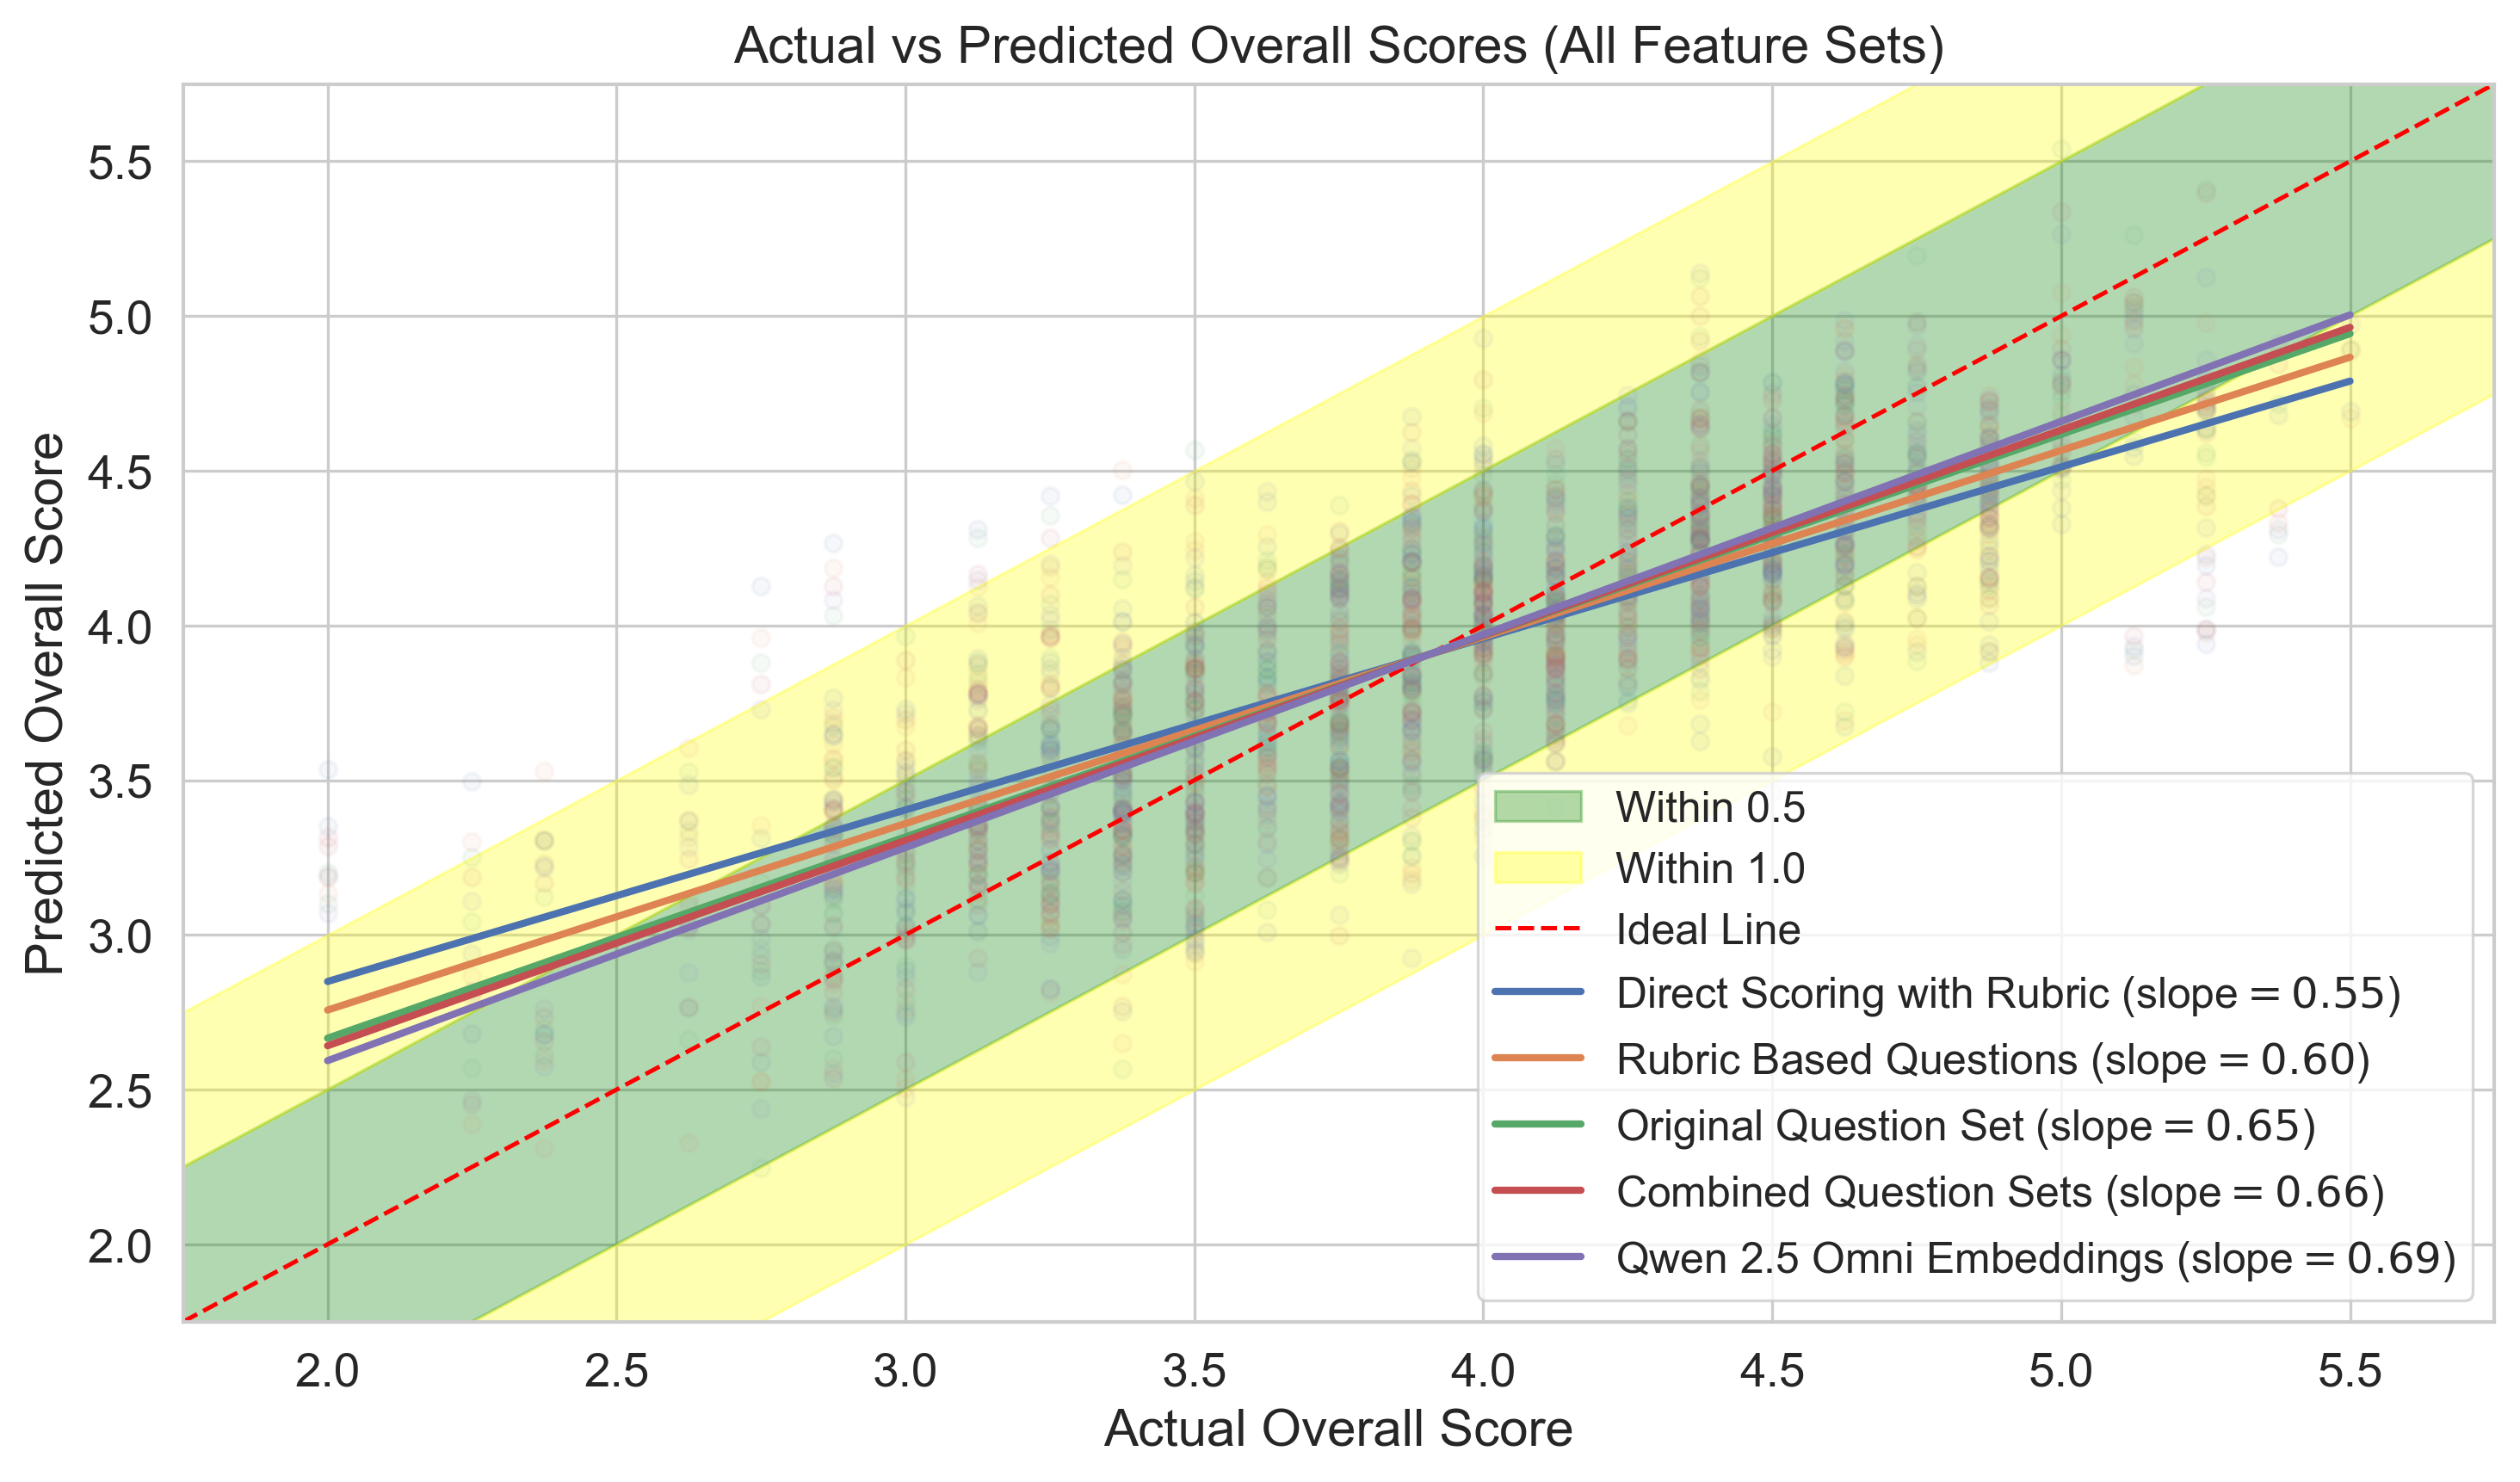
\includegraphics[width=1\linewidth]{images/actual_vs_predicted_all.png}
  \caption{Regression lines of predictions versus ground truth scores across all feature sets. The plots show how different feature representations affect the regression line, with higher-dimensional features with higher PCC generally producing larger slopes that are able to better capture extreme target values.}
  \label{fig:predictions_vs_ground_truth_all}
\end{figure}

\section{Interpretable Feature Analysis}
\label{sec:interpretable_feature_analysis}
In this section, we analyze the interpretable features extracted by our question-based approach to understand their relationships with each other and the target variable to extract useful insights.

\subsection{Correlation Analysis}
\label{subsec:correlation_analysis}
We begin by examining the correlation structure between features and the target variable - part score.

\begin{figure}[h]
  \centering
  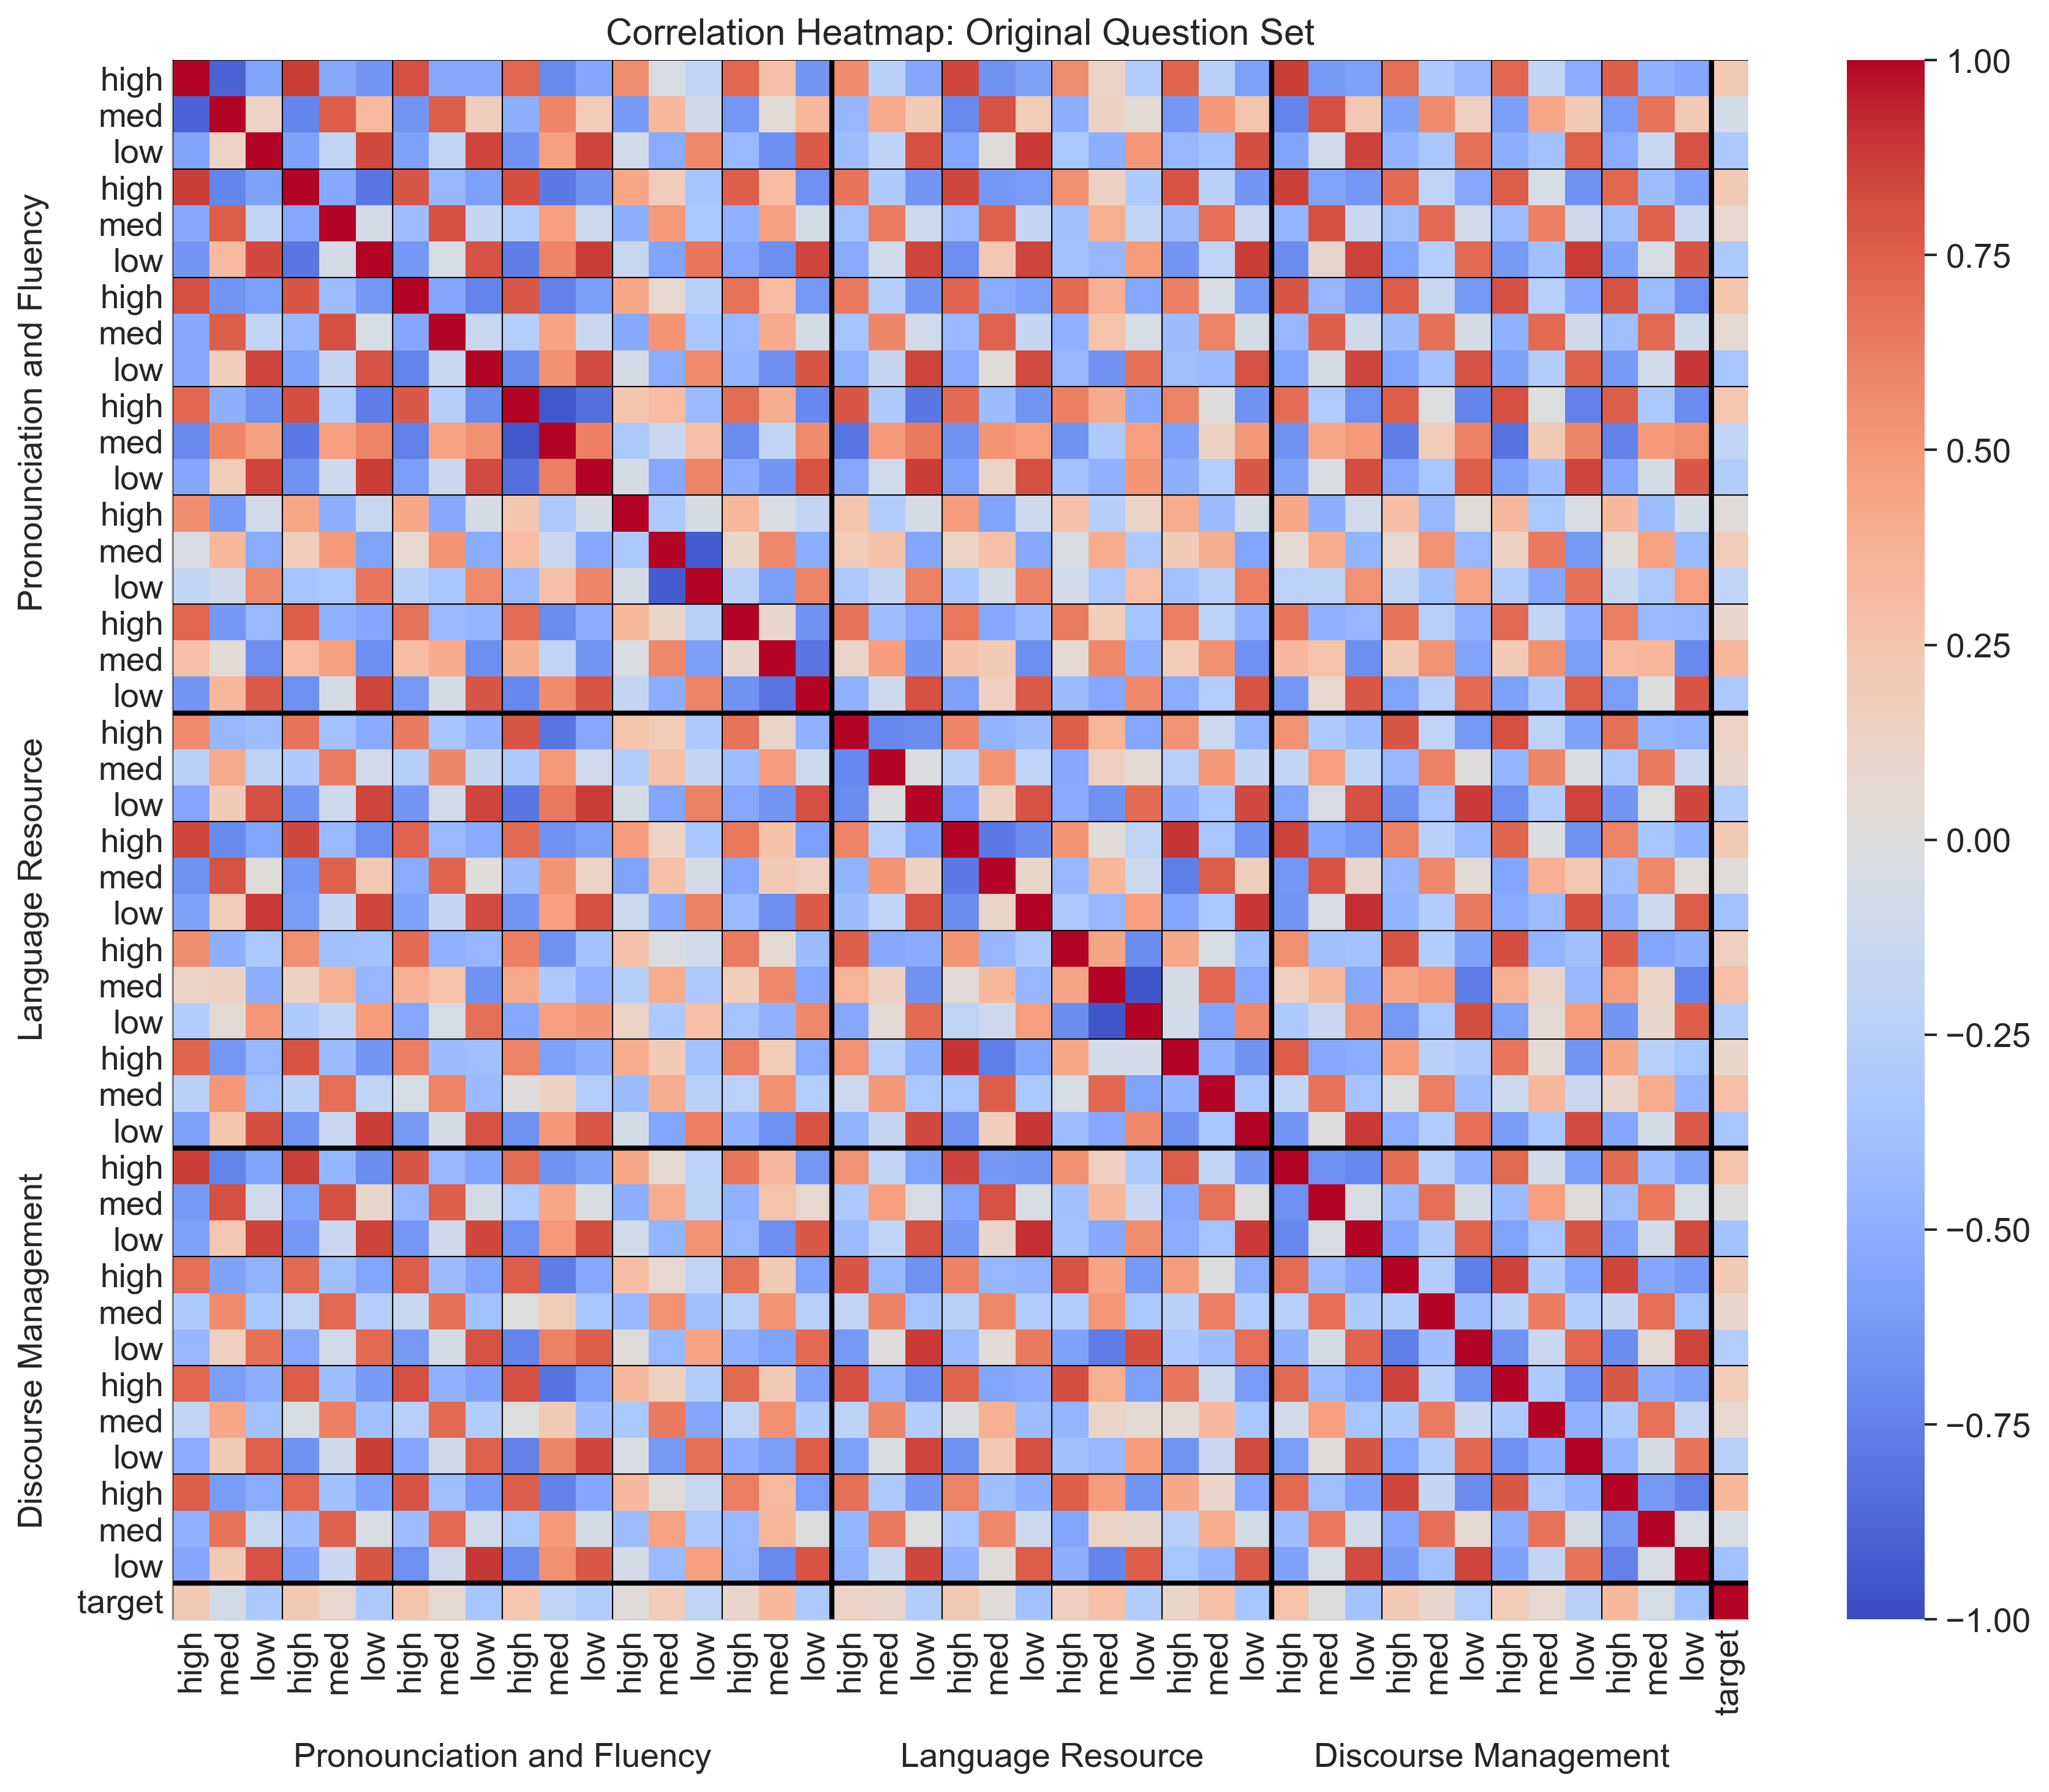
\includegraphics[width=1\linewidth]{images/correlation_matrix_original.png}
  \caption{Correlation matrix between features and the target variable from the \emph{Initial Question Set}. Each question has three features corresponding to the probabilities of the ``High'', ``Medium'', and ``Low'' options.}
  \label{fig:correlation_matrix_original}
\end{figure}

Figure \ref{fig:correlation_matrix_original} presents the correlation matrix for the \emph{Initial Question Set}, revealing several important patterns. As expected, features exhibit intuitive correlations with part scores: ``High'' features correlate positively with the scores, ``Low'' features correlate negatively, and ``Medium'' features show mixed correlations depending on the specific question. 

Additionally, we observe that ``High'' features are generally positively correlated with other ``High'' features and negatively correlated with Low features. Interestingly, these correlations seem to transcend rubric dimensions; for example, pronunciation and fluency questions show strong correlations with language resource questions. This could suggest that the speech LLM struggles to effectively distinguish between different dimensions of speaking proficiency, or it may reflect inherent correlations in the data itself, for example that candidates who speak more fluently also tend to use a wider range of vocabulary and grammar. That being said, the cross-dimension correlations seem to be slightly lower than within-dimension correlations, indicating that the speech LLM retains some ability to differentiate between different aspects of speaking proficiency.

Furthermore, some questions, such as pronunciation and fluency question 5, appear less correlated with others and also show weaker correlations with part scores, indicating they may contribute less predictive value to the overall assessment. Overall, the correlation analysis reveals high levels of multicollinearity across the feature set.

Figure \ref{fig:correlation_matrix_rubric} shows the correlation matrix for the \emph{Rubric-based Question Set}.

\begin{figure}[h]
  \centering
  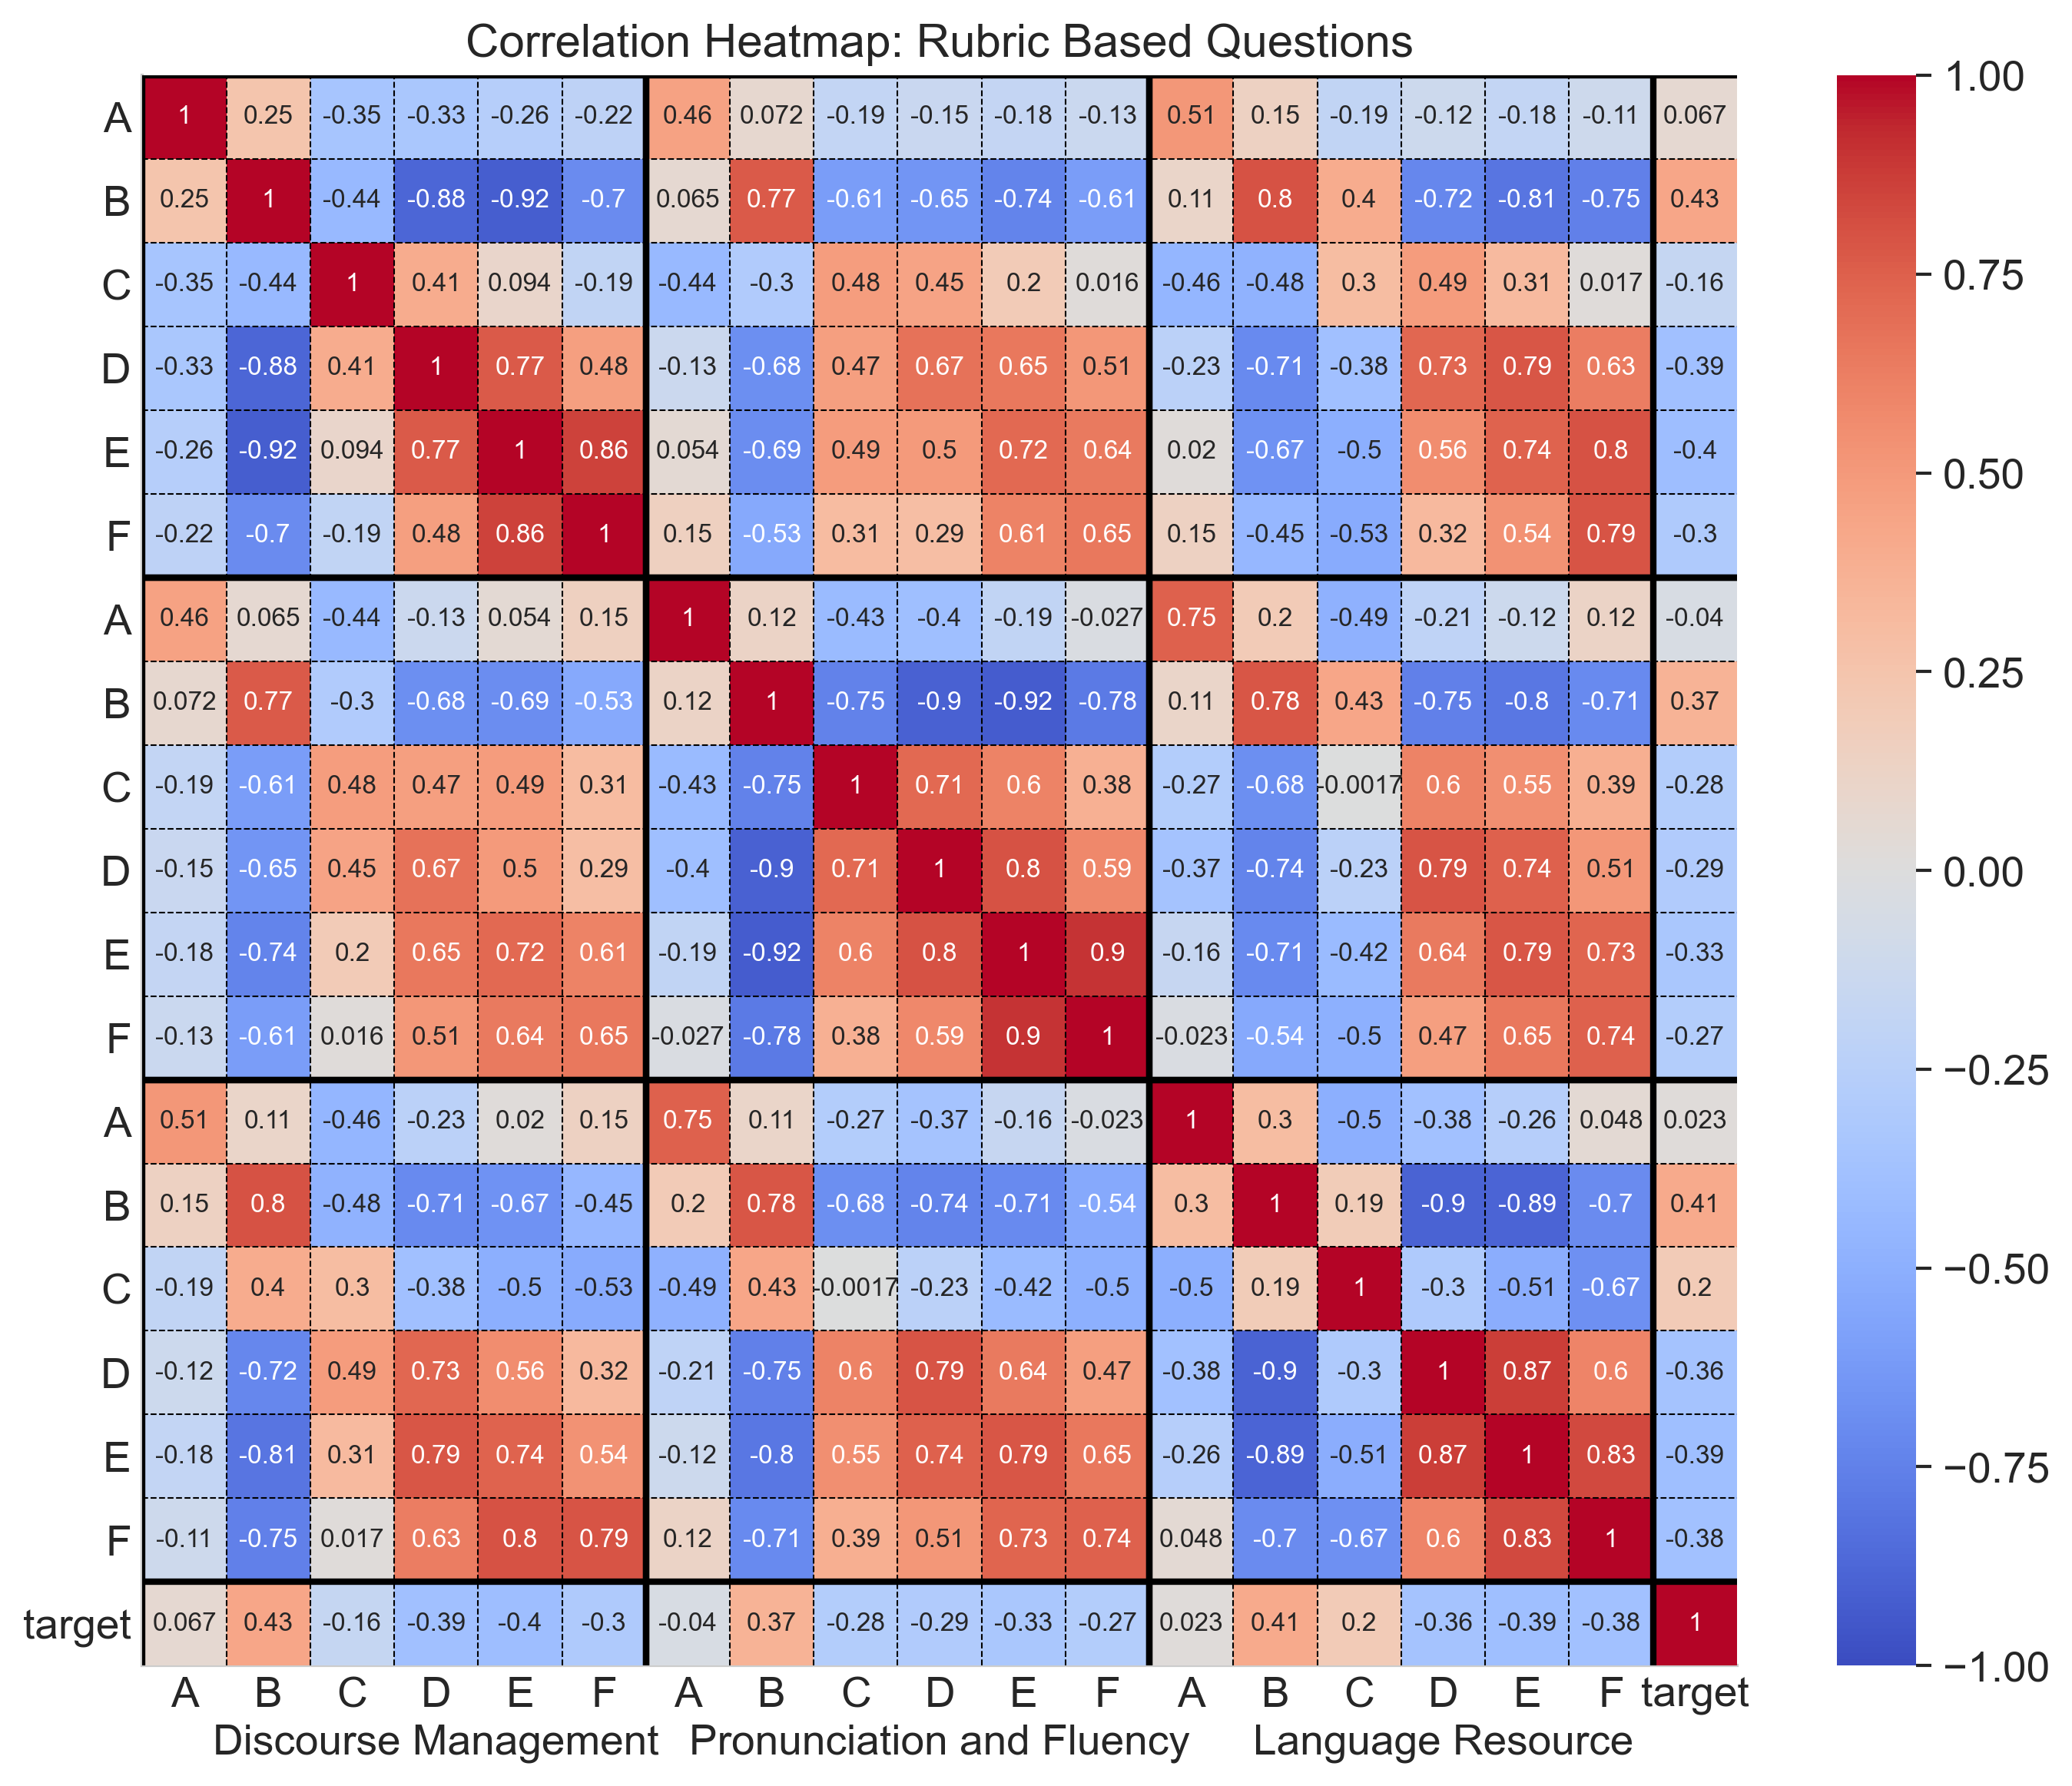
\includegraphics[width=1\linewidth]{images/correlation_matrix_rubric.png}
  \caption{Correlation matrix between features and the target variable from the \emph{Rubric-based Question Set}. Each rubric dimension has six features corresponding to the probabilities of grades A through F.}
  \label{fig:correlation_matrix_rubric}
\end{figure}

Grade A features exhibit very weak correlations with part scores, indicating that the speech LLM rarely assigns high probability to this option. Grade B features demonstrate the strongest positive correlations, while Grades C, D, and E show progressively more negative correlations. Grade F shows slightly less negative correlation than Grade E, likely due to similarly low assignment probabilities. Overall, the weaker alignment between feature correlations and prior expectations may stem from the increased number of response options (6 vs 3), which can lead to small and uninformative probability values assigned to extreme grades. Importantly, while grades show correlation across rubric dimensions, these cross-dimensional correlations are again weaker than within-dimension correlations, indicating that the speech LLM retains some ability to differentiate between different aspects of speaking proficiency.

\subsection{Regression Coefficients}
\label{subsec:regression_coefficients}
Analysis of the regression coefficients for the \emph{Rubric-based Question Set} reveals coefficients whose signs contradict intuitive expectations derived from correlation analysis, as illustrated in Figure \ref{fig:regression_coefficients}. This counter-intuitive behaviour stems from the high degree of multicollinearity present among the extracted features. For example, Discourse Management Grade B has a strongly negative coefficient while Language Resource Grade B has a strongly positive coefficient, despite both showing similar correlation patterns with the target scores. Increasing the regularization parameter in ridge regression to mitigate multicollinearity makes coefficients more aligned with intuitive expectations, but this comes at the cost of significantly degraded model performance as excessive regularization effectively reduces the model to a constant predictor.

\begin{figure}[h]
  \centering
  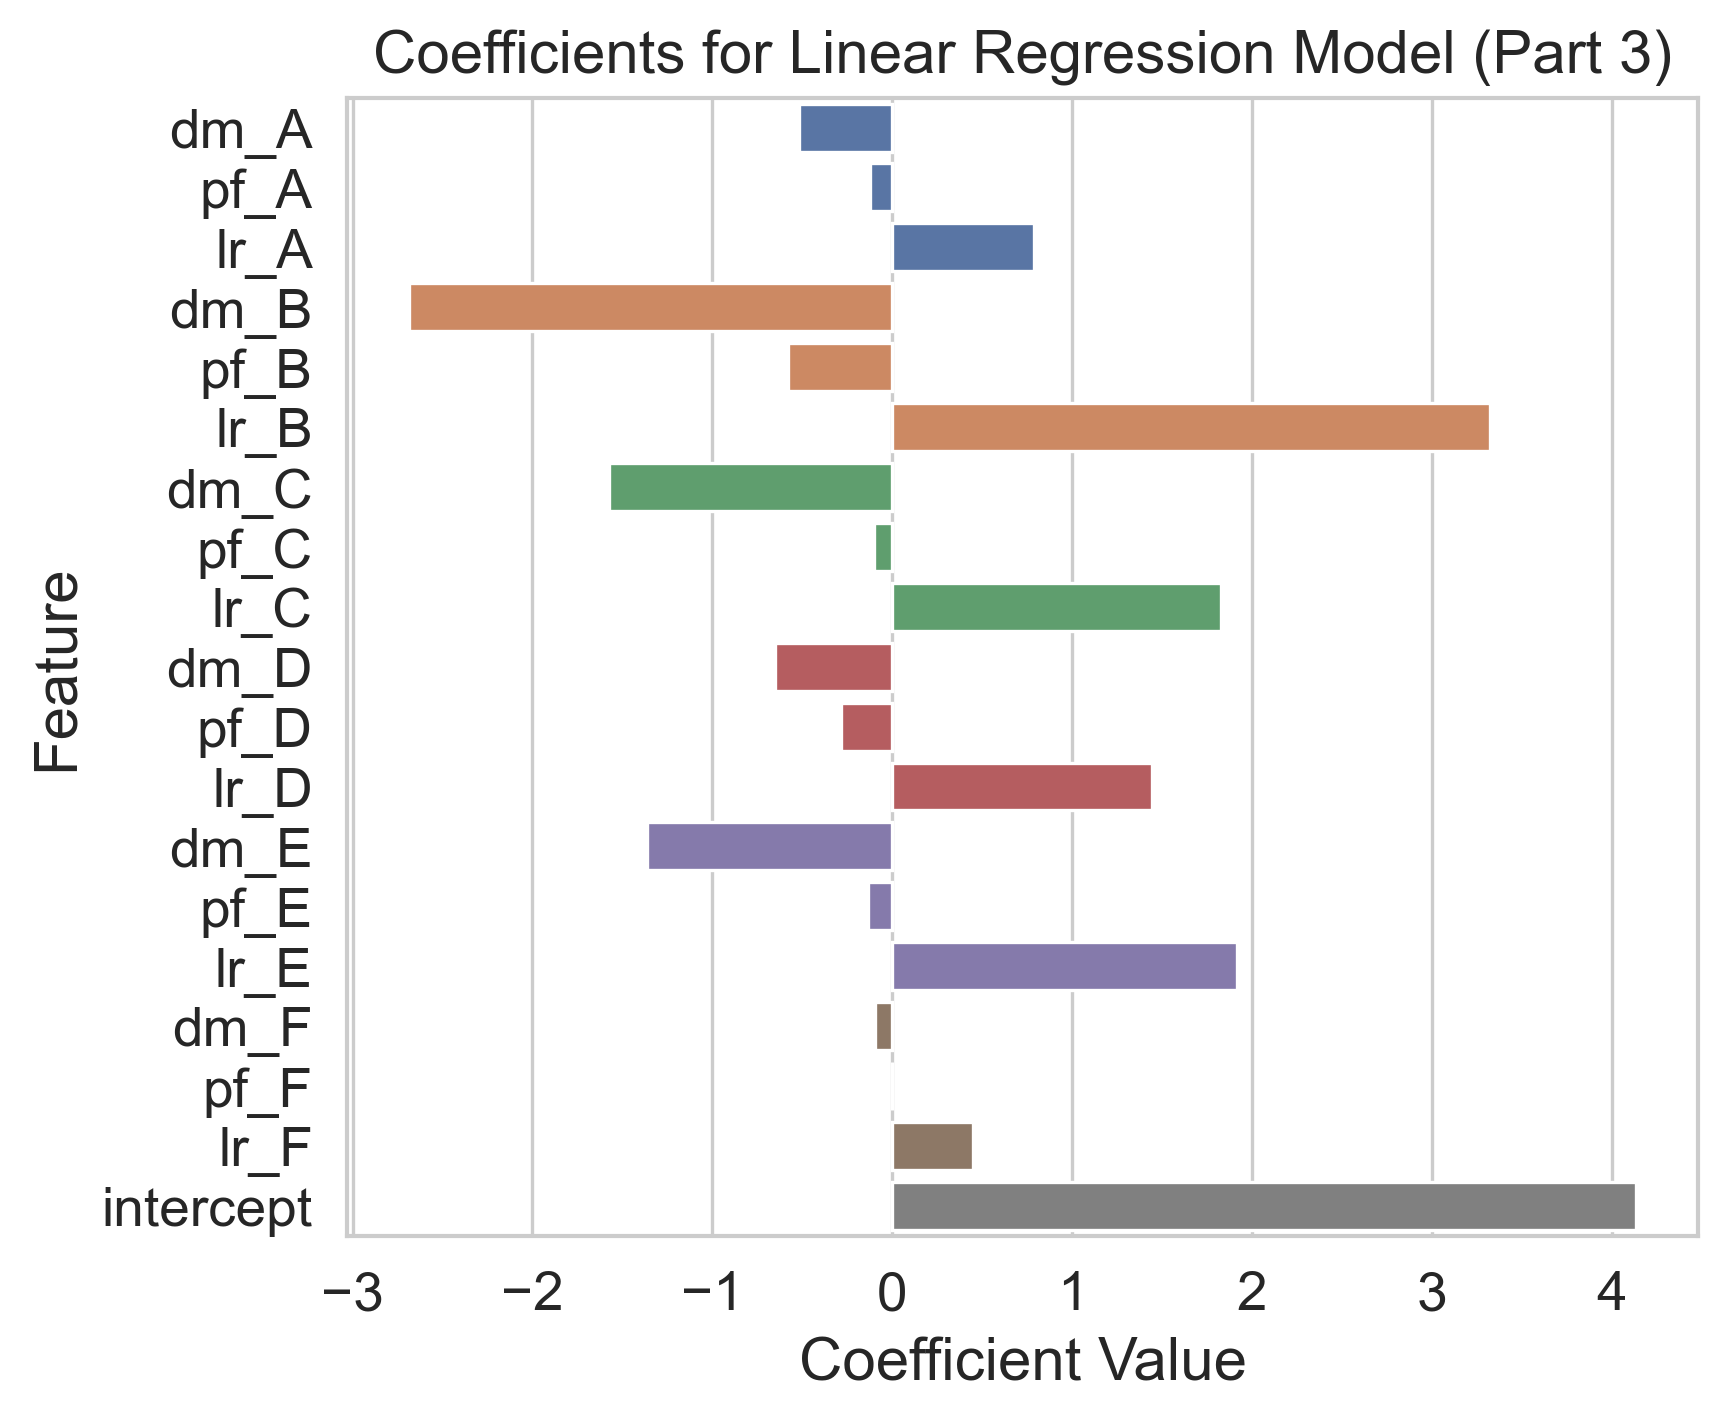
\includegraphics[width=0.8\linewidth]{images/coefficients.png}
  \caption{Regression coefficients for the \emph{Rubric-based Question Set}. Each rubric dimension (pronunciation and fluency: pf, language resource: lr, discourse management: dm) has six grade options (A-F). The counter-intuitive coefficient signs demonstrate that high-grade features (A) don't consistently receive positive coefficients, and low-grade features (F) don't consistently receive negative coefficients, illustrating the impact of multicollinearity among features.}
  \label{fig:regression_coefficients}
\end{figure}

\subsection{Question-level Scores}
\label{subsec:question_scores}
To address the interpretability challenges posed by multicollinearity while maintaining the pedagogical value of our approach, we implement an alternative interpretation strategy. We train separate linear regression models to predict part scores using only features corresponding to each individual rubric dimension. The predictions from these dimension-specific models can be interpreted as analytic scores for each rubric criterion, effectively decomposing the holistic scores into predicted analytic scores. We call these predictions \textbf{question-level scores}, as they represent the model's assessment of a candidate's performance specific to each question. The variability amongst these question-level scores provides insights into the candidate's strengths and weaknesses across different dimensions of speaking proficiency. This methodology is illustrated in Figure \ref{fig:question_level_methodology}.

\begin{figure}[h]
  \centering
  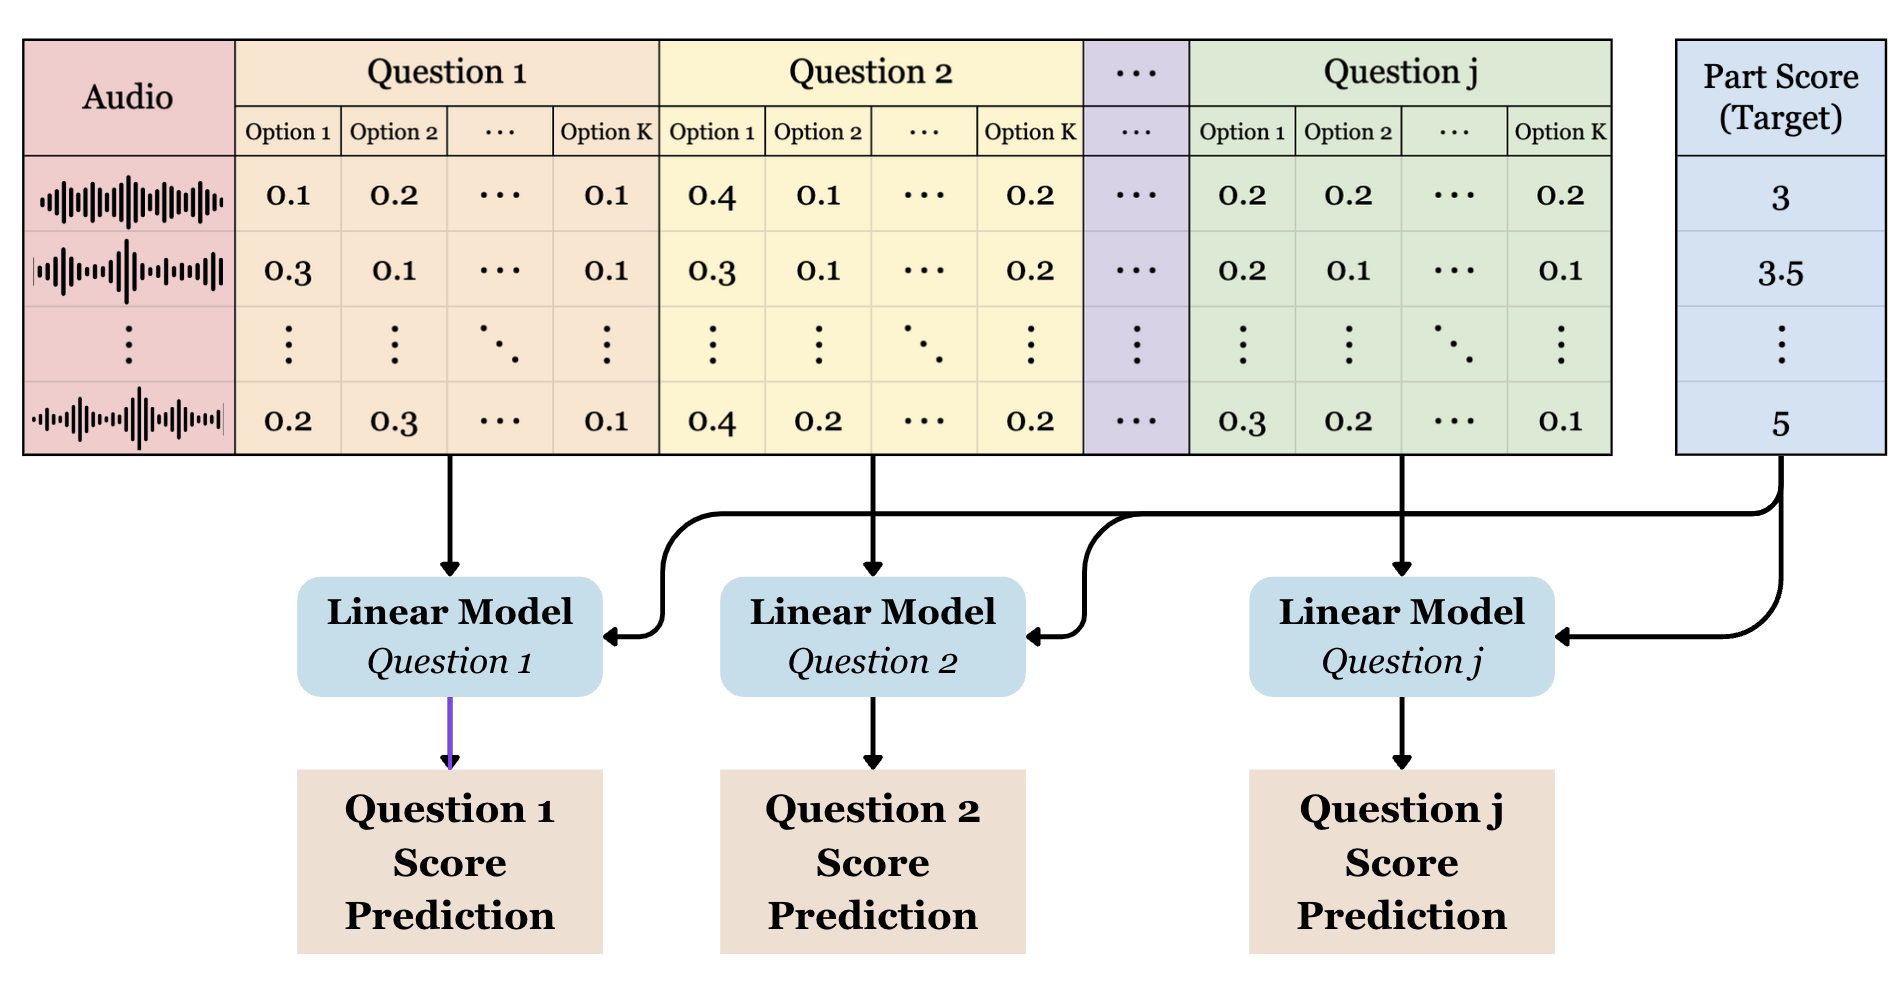
\includegraphics[width=1\linewidth]{images/question_scores_schematic.png}
  \caption{Illustration of the question-level scores methodology for obtaining analytic scores for each question. Separate linear models are trained to predict the same target variable (part score) for each question using only features corresponding to that question, and the predictions from these models are interpreted as question-level scores.}
  \label{fig:question_level_methodology}
\end{figure}

\begin{figure}[h]
  \centering
  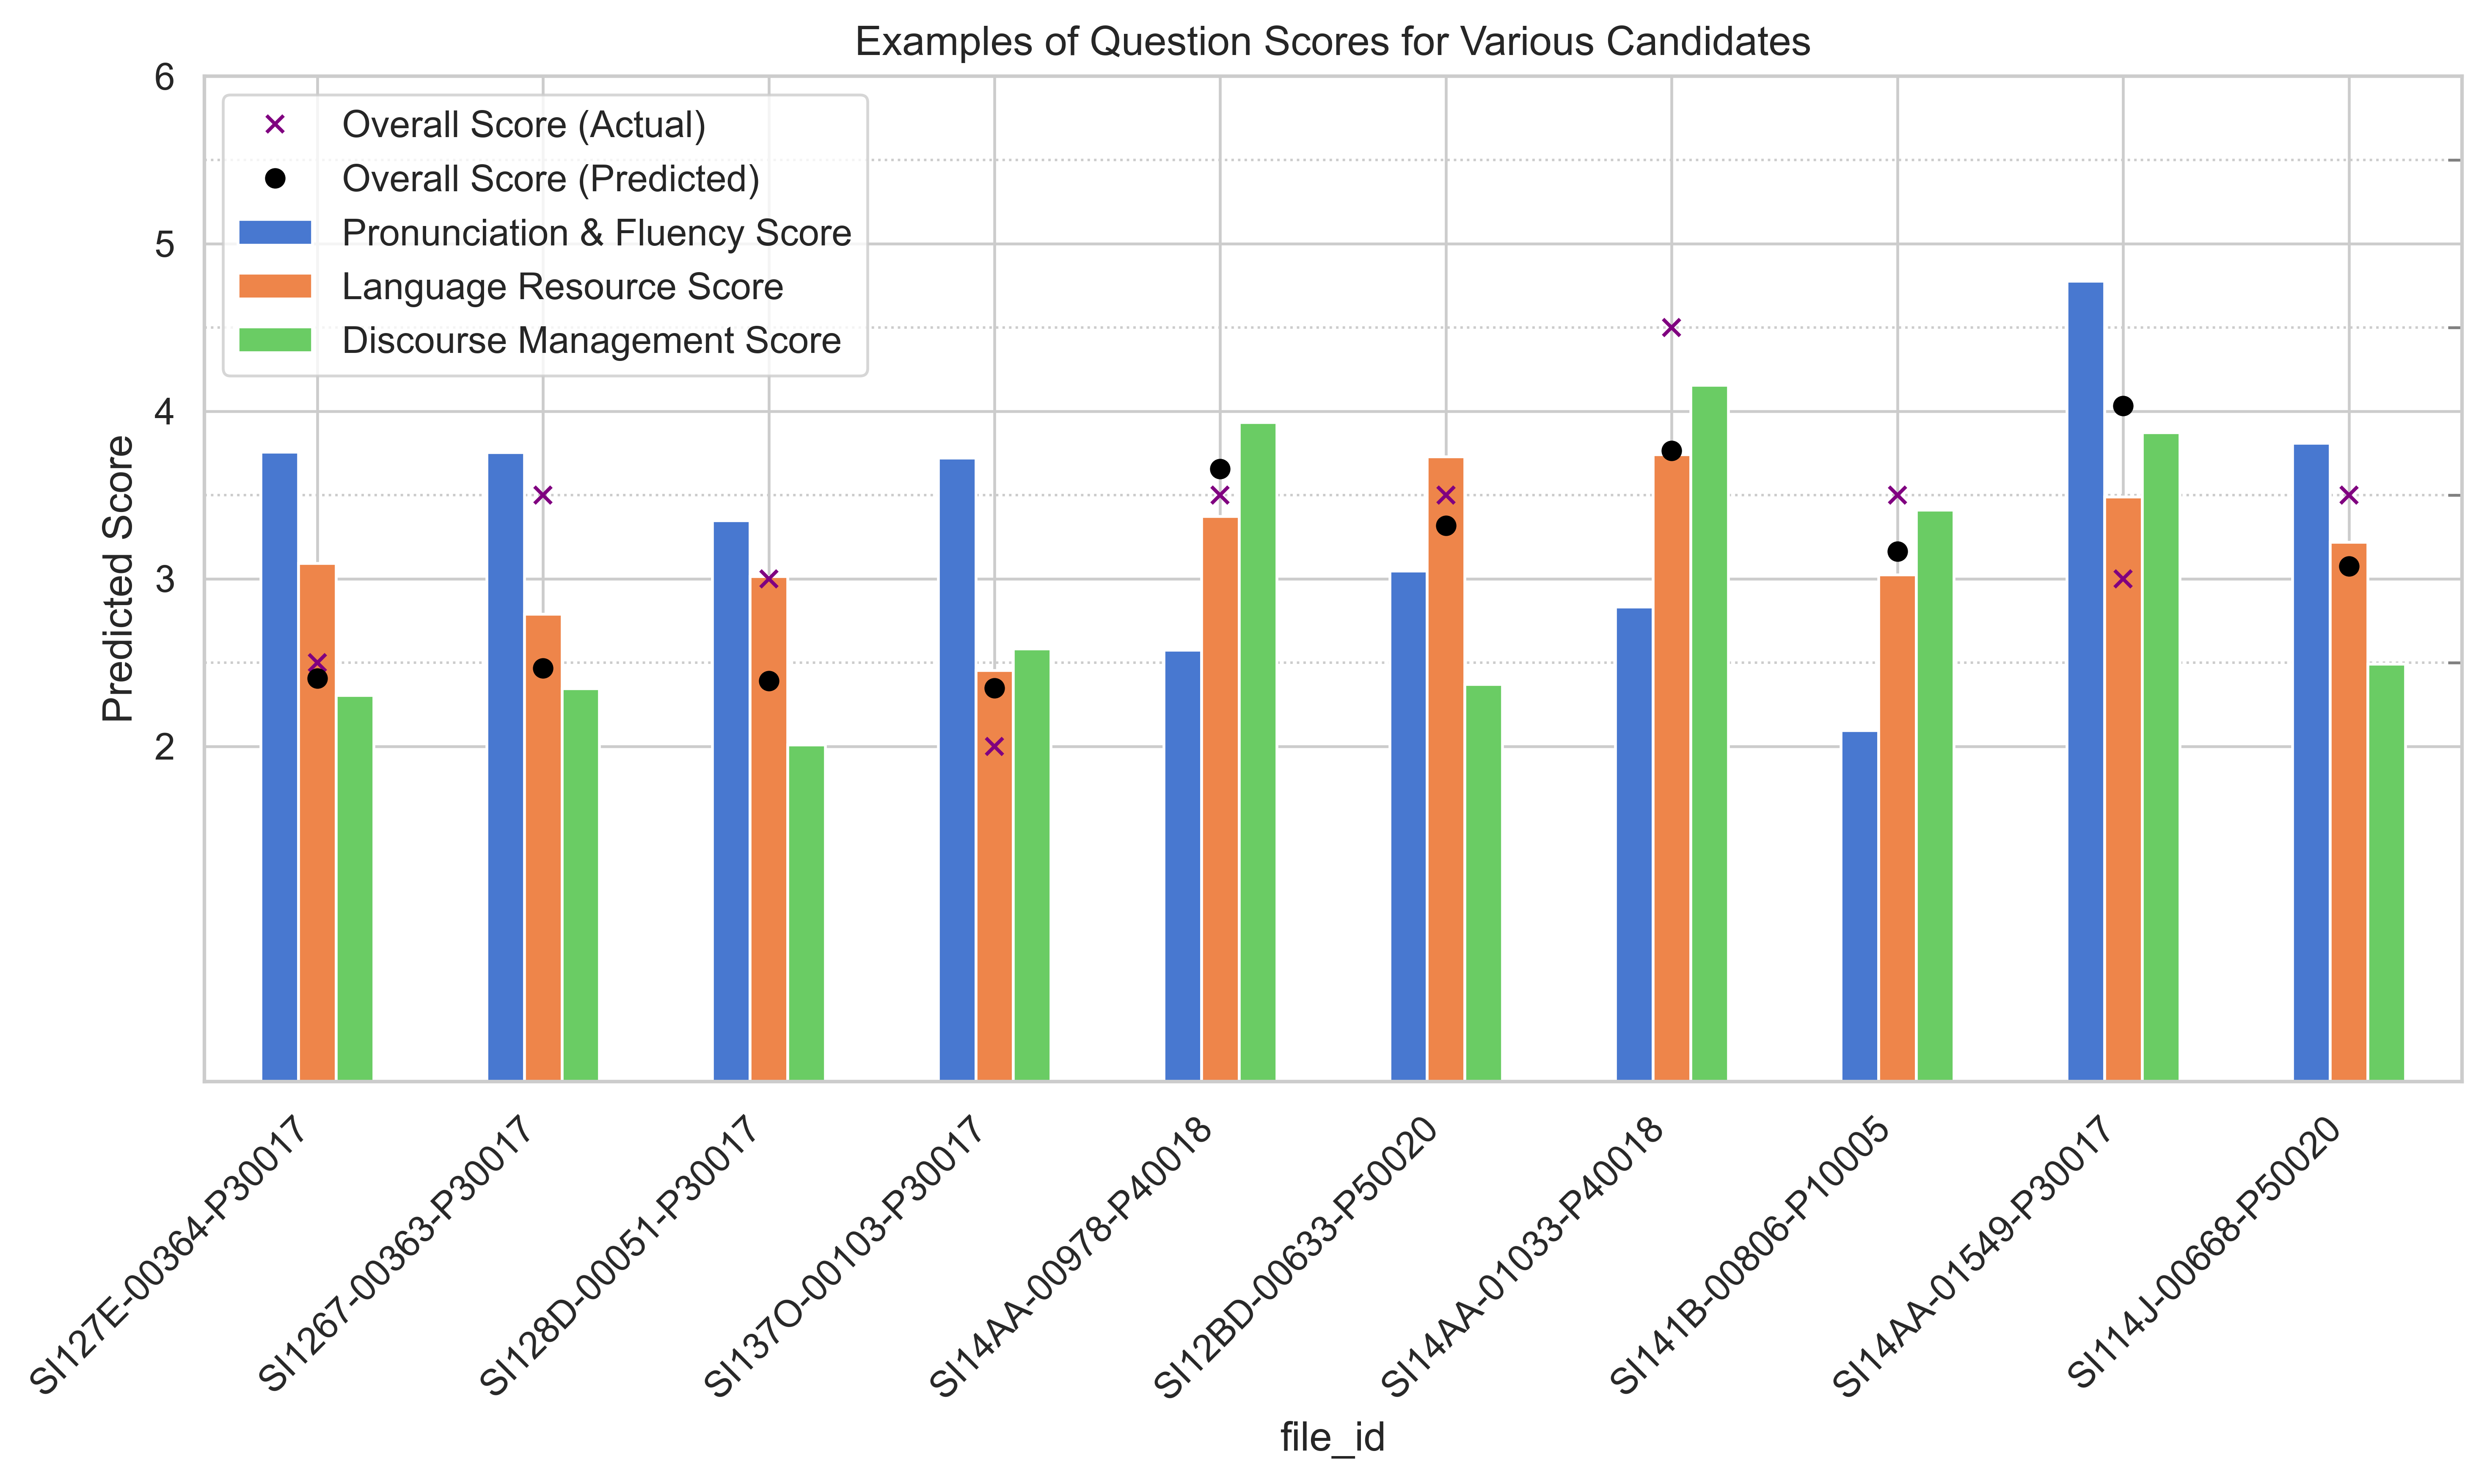
\includegraphics[width=1\linewidth]{images/question_score_examples.png}
  \caption{Question-level scores for different rubric dimensions across various sample candidates, illustrating how each criterion contributes to the overall assessment. Each file ID corresponds to a candidate's response for a specific test component.}
  \label{fig:analytic_scores}
\end{figure}

Figure \ref{fig:analytic_scores} visualizes these dimension-specific predictions for various candidates, showing how each rubric criterion contributes to the overall assessment. This visualization proves especially valuable for educational applications, as it enables candidates to receive targeted feedback on their performance across different dimensions of speaking proficiency. Rather than receiving only a holistic score, learners can identify specific areas for improvement, such as pronunciation and fluency, language resource usage, or discourse management, facilitating more effective and focused practice strategies.

\section{Low Data Regime}
\label{sec:low_data_regime}
In this section, we investigate the scalability of speech LLM-based SLA, something that has not been studied in prior work. We evaluate the performance of the \emph{Initial Question Set}, \emph{Direct Scoring Question}, \emph{Rubric-based Question Set}, and the \emph{Speech LLM Representations} in simulated low data regimes by training models on various fractions of the training data and evaluating performance on the dev set. Specifically, we train models on 0.2\% to 100\% of the training data (approximately 6 to 3000 samples) and evaluate performance on the full dev set. Each experiment is repeated 100 times with different random seeds to account for variability in training data selection. We employ ridge regression with regularization strength selected via cross-validation on the training set for all models to ensure robustness even in low data regimes where the number of features may approach or greatly exceed the number of training samples. We report performance in terms of mean PCC and RMSE over the 100 trials for each training data fraction with standard deviations obtained from the performance variability within the 100 trials.

\begin{figure}[h]
  \centering
  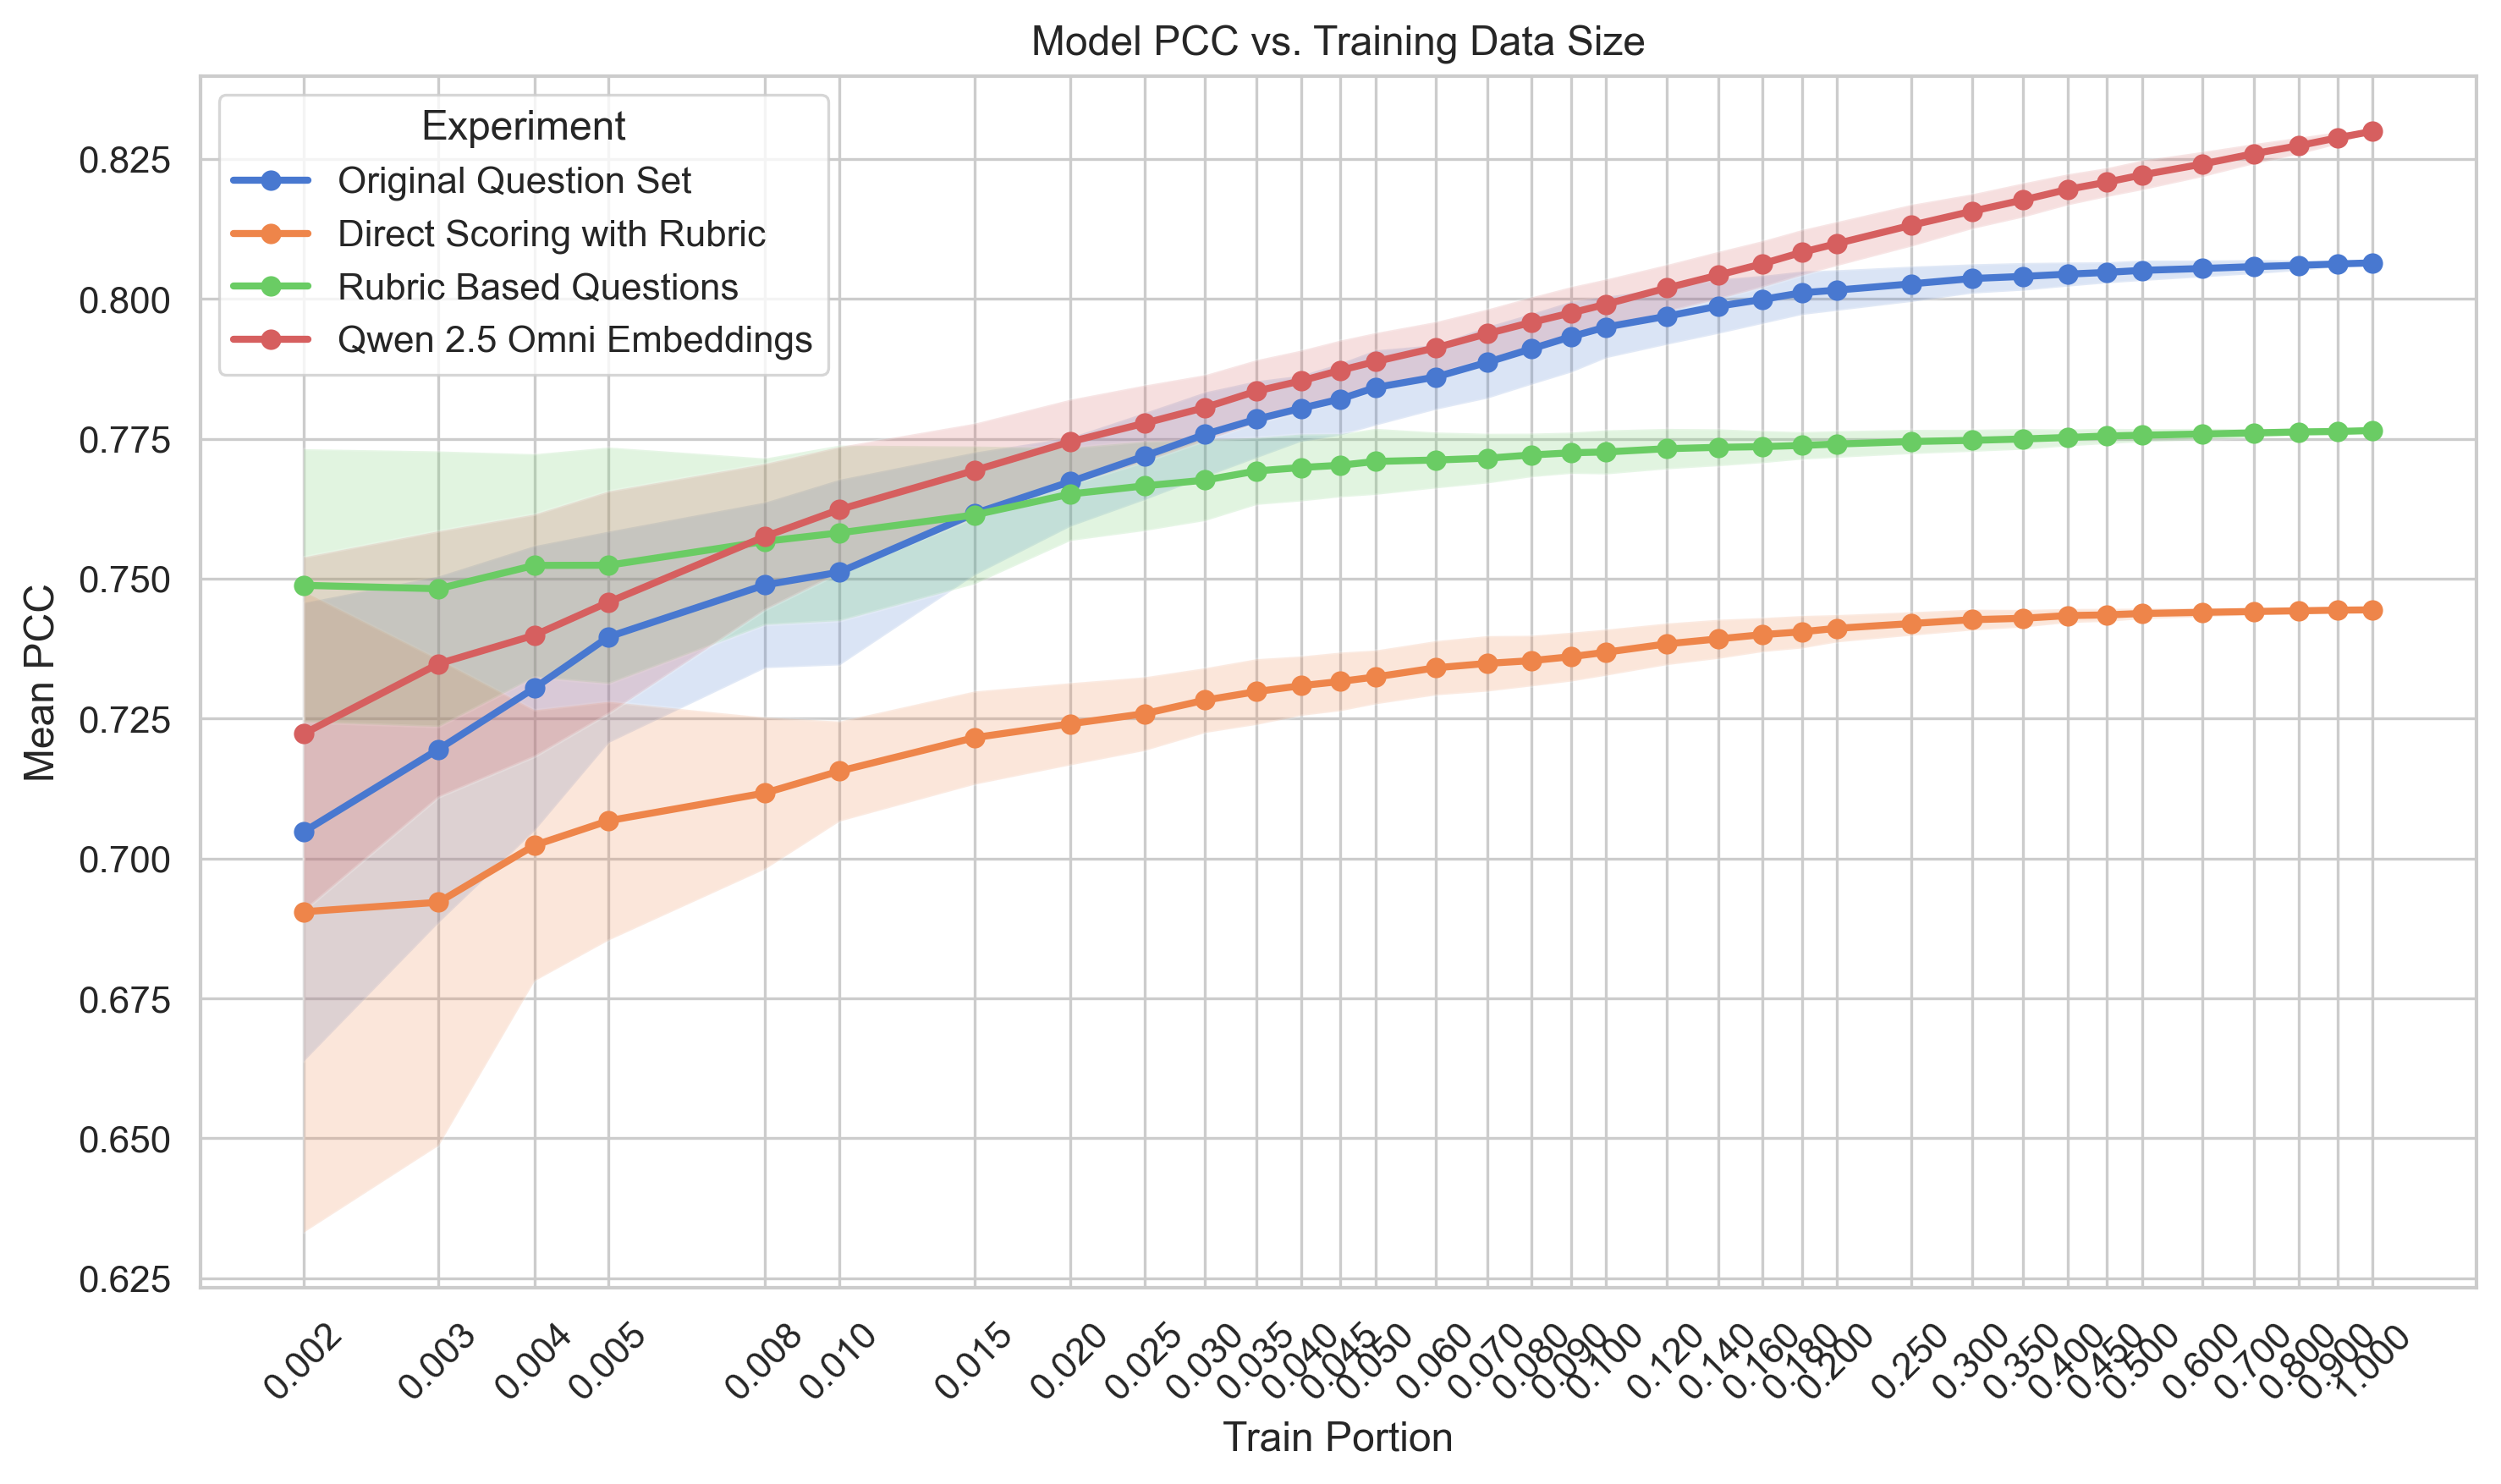
\includegraphics[width=1\linewidth]{images/low_data_regime_pcc.png}
  \caption{Scaling curves showing PCC as a function of training data size (log scale) across different feature sets. Each point represents the mean performance over 100 random sub-samples of the training data, with the shaded region indicating the standard deviation across the 100 sub-samples.}
  \label{fig:low_data_regime_pcc}
\end{figure}

\begin{figure}[h]
  \centering
  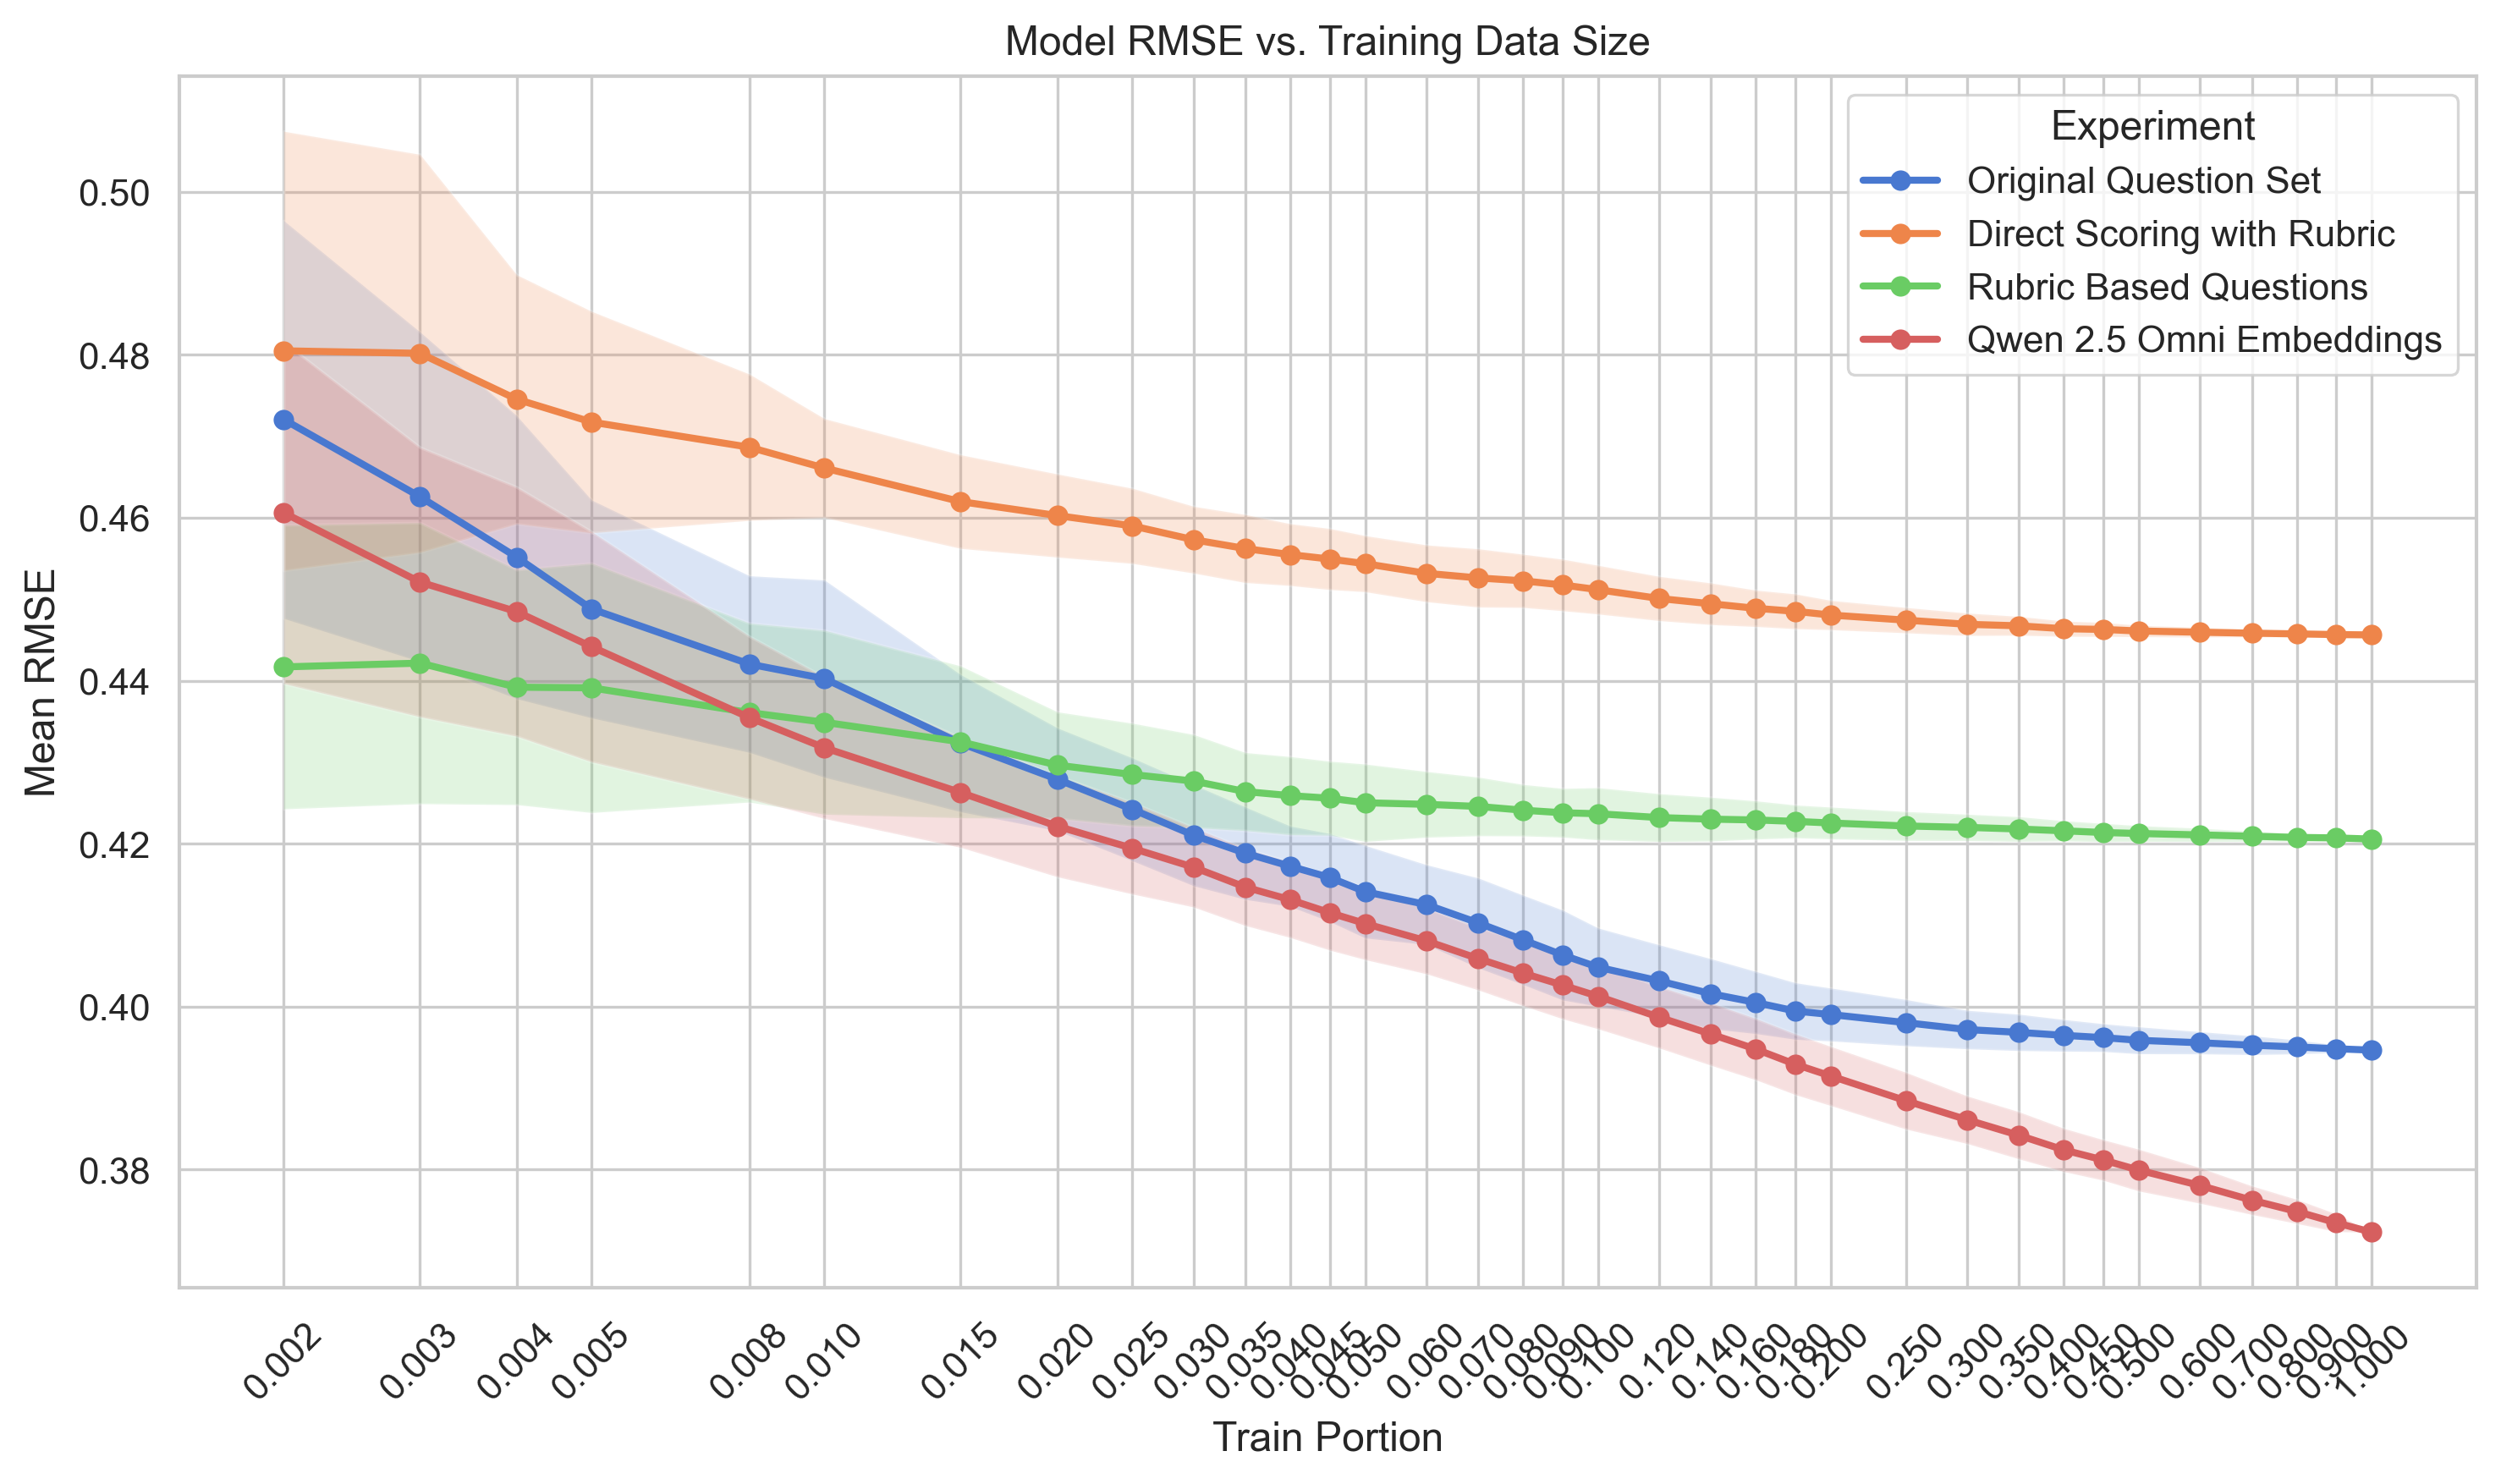
\includegraphics[width=1\linewidth]{images/low_data_regime_rmse.png}
  \caption{Scaling curves showing RMSE as a function of training data size (log-scale) across different feature sets. Each point represents the mean performance over 100 random sub-samples of the training data, with the shaded region indicating the standard deviation across the 100 sub-samples.}
  \label{fig: fig:low_data_regime_rmse}
\end{figure}

Figures \ref{fig:low_data_regime_pcc} and \ref{fig: fig:low_data_regime_rmse} present the scaling curves for PCC and RMSE, respectively, revealing several important insights about the data efficiency of different feature representations.

Most remarkably, the \emph{Rubric-based Question Set} demonstrates exceptional performance in extremely low data regimes. With only 0.2\% of training data (approximately 6 samples), it achieves a PCC around 0.75 and RMSE around 0.44, which is comparable to the \emph{BERT Baseline} trained on the full dataset. This suggests that speech LLMs can extract highly relevant information for scoring without requiring large amounts of training data, and that a well-chosen question set can enable effective SLA by guiding the model to focus on the most relevant aspects of the underlying audio representation. The superior performance of the \emph{Rubric-based Question Set} compared to other question-based approaches in this regime indicates that specific question design is critical, and that simply having more questions or options does not necessarily improve performance when training data is scarce.

Beyond approximately 0.8\% of training data, the relative performance rankings stabilize, with more comprehensive feature sets generally achieving better performance. The \emph{Speech LLM Representations} consistently outperform all question-based feature sets across all data regimes, while among the question-based approaches, the \emph{Initial Question Set} (42 features) surpasses the \emph{Rubric-based Question Set} (18 features) once sufficient training data becomes available. Interestingly, the question-based approaches appear to reach performance plateaus around 30\% of the training data, while the \emph{Speech LLM Representations} continue to improve with additional data, suggesting that question-based methods may have inherent asymptotic performance limitations compared to the full representational capacity of speech LLM embeddings.

The scaling curves also reveal substantially higher performance uncertainty in low data regimes, as evidenced by the larger standard deviations across trials. This increased variability indicates that the specific selection of training samples has a more pronounced impact on model performance when training data is limited, highlighting the importance of careful data curation in resource-constrained scenarios.

\chapter{Conclusion}
\label{chap:conclusion}
This dissertation sought to answer the research question: \textbf{Can speech Large Language Models be used to develop interpretable systems for automatic spoken language assessment while maintaining competitive predictive performance?} Through multiple experiments on the Speak \& Improve Corpus 2025, we investigated the effectiveness of question-based interpretable features derived from speech LLMs for automatic spoken language assessment (SLA).

\section{Summary of Findings}
Our question-based interpretable SLA approach achieves competitive performance with dramatically fewer features, attaining a PCC of 0.8052 with just 42 interpretable features compared to the black-box \emph{Speech LLM Representation}'s PCC of 0.8282 with 3584 features. However, the direct use of speech LLM embeddings as features still outperforms our question-based approach across all configurations. Notably, combining question-based features with speech LLM embeddings yields no significant performance improvements, suggesting that our question-based method doesn't extract fundamentally new information but rather picks out relevant aspects from the same underlying audio representation in an interpretable manner.

Our experiments with feature transformations reveal that exponentiated features (probabilities) perform best, while discrete features perform significantly worse, indicating that the richer information contained in probability distributions is crucial for performance. The strong performance of simple linear regression models, comparable to more complex approaches like SVR and neural networks, demonstrates that the relationship between extracted features and final scores is largely linear. We also find that more questions generally lead to better performance, with PCC improving from 0.7427 for the \emph{Direct Scoring Question} to 0.8052 for 14 questions in the \emph{Initial Question Set}. Similarly, more options per question appear to improve performance, but with an important caveat: too many options can lead to extreme options consistently receiving low probabilities and becoming uninformative, as observed in the \emph{Rubric-based Question Set}. Regarding inference strategy, batch inference only slightly underperforms individual inference (PCC decrease of ~0.003-0.005), making it a viable option when computational efficiency is a priority.

Our correlation analysis reveals high multicollinearity among question-based features, even across different rubric dimensions, complicating the interpretation of regression coefficients which often display counter-intuitive signs. This multicollinearity could indicate that the speech LLM struggles to effectively distinguish between different dimensions of speaking proficiency, or it may reflect inherent correlations in the data itself, such as candidates who speak more fluently also tending to use more sophisticated vocabulary. To address these interpretability challenges, we propose fitting separate regression models on features corresponding to each question to obtain question-level scores. These question-specific predictions effectively decompose holistic scores into analytic scores, providing valuable insights into candidates' strengths and weaknesses across different aspects of speaking proficiency.

In terms of scalability, the \emph{Rubric-based Question Set} demonstrates exceptional performance in extremely low data regimes, achieving a PCC around 0.75 with just 0.2\% of training data (approximately 6 samples), comparable to the \emph{BERT Baseline} trained on the full dataset, and outperforming \emph{Speech LLM Representations} in this regime in this regime. This suggests that speech LLMs can extract highly relevant information for scoring without requiring large amounts of training data, and that a well-chosen question set can enable effective SLA by guiding the model to focus on the most relevant aspects of the underlying audio representation. However, other question-based approaches do not perform as well in this regime, indicating that specific question design is critical.

Overall, these results collectively highlight the trade-off between interpretability and predictive accuracy in automated spoken language assessment, while demonstrating the viability of question-based interpretable features even in resource-constrained scenarios.

\section{Implications for SLA and Educational Technology}
Our question-based approach enables targeted feedback by decomposing holistic scores into interpretable dimensions such as pronunciation, fluency, and language resource usage. This allows learners to identify specific weaknesses and focus practice efforts on areas most likely to yield improvement, while educators can design personalized interventions based on individual learner profiles. The transparency of assessment criteria makes evaluation more understandable and actionable compared to black-box systems that provide only unexplained holistic scores.

The data efficiency demonstrated in our experiments—competitive performance with just 10\% of training data—significantly reduces barriers to developing SLA systems. This makes automated assessment feasible for less-resourced languages and specialized domains where extensive annotated datasets are unavailable, potentially democratizing access to high-quality spoken language assessment tools worldwide.

\section{Limitations and Future Work}
A fundamental limitation of our approach is the lack of guarantees that the extracted interpretable features truly capture the intended linguistic concepts they are designed to assess. While our correlation analysis and the success of similar methodologies in other domains provide some evidence for conceptual alignment, we cannot definitively establish that high probabilities for "pronunciation quality" features genuinely reflect superior pronunciation rather than other correlated factors. Future work should conduct comprehensive validation studies comparing our automatically generated question-level scores with expert assessments on the same dimensions, potentially through expert annotation of the specific traits our questions target.

The design of effective question sets remains a significant challenge. Our questions were developed through a combination of expert knowledge and LLM assistance, but creating question sets that are both comprehensive and yield disentangled features represents an open research problem. The high multicollinearity observed in our extracted features demonstrates the difficulty of designing questions that capture distinct aspects of proficiency while maintaining predictive power. Future work could explore automatic question generation through prompt optimization techniques, potentially using iterative refinement based on feature independence criteria or predictive performance on held-out data.

The question-based methodology we propose demonstrates considerable generality and could be readily adapted to other modalities and assessment tasks. Beyond spoken language assessment, this approach could be applied to any regression or classification task on unstructured data where interpretability is desired. Furthermore, similar approaches could be employed in other modalities such as pure text, images, or videos. The core principle of decomposing complex evaluation tasks into structured, interpretable sub-questions represents a promising direction for developing explainable AI systems across domains where human-interpretable feedback is crucial.

An important limitation of our analysis is that we lack the domain expertise to conduct meaningful error analysis at the individual candidate level. While we attempted to examine specific examples where different models achieved varying levels of accuracy—identifying cases where our question-based approach succeeded or failed relative to baseline methods—we were unable to discern meaningful patterns in these differences. Without deep expertise in spoken language assessment and the nuanced factors that influence human grader decisions, we could not determine why certain candidates received lower scores than others or why specific models performed better on particular types of responses. This limitation highlights the importance of involving domain experts in future research, particularly for conducting qualitative error analysis that could reveal insights into model behaviour and guide improvements to question design and feature extraction strategies.

Finally, bias and fairness considerations, while not explicitly studied in this work, represent critical concerns for any deployed assessment system. Future research should systematically investigate whether speech LLM-based features exhibit differential performance across demographic groups, including but not limited to native language background, gender, age, and socioeconomic status. The interpretable nature of our question-based features may actually provide advantages in this regard, as biased model behaviour could be more easily identified and addressed through targeted interventions on specific questions rather than requiring modifications to opaque black-box systems. Developing bias detection and mitigation strategies specifically tailored to question-based interpretable features represents an important avenue for ensuring equitable deployment of automated assessment technologies.

\appendix

\bibliographystyle{plainnat}
\bibliography{references}

\chapter{Full Question Sets and Prompts}
\label{app:full_question_sets}
In this chapter, we provide the full question sets and text prompts used in our experiments.

\section{Initial Question Set}
\label{app_sec:initial_question_set}
In this section, we list all the questions in the \emph{Initial Question Set}. The questions are divided into three categories: Pronunciation and Fluency, Language Resource, and Discourse Management. Each question has three response options: ``High'', ``Medium'', and ``Low''.

% Pronunciation and Fluency
\subsection*{Pronunciation and Fluency}
\begin{enumerate}
  \item \textbf{Intelligibility — Can an average listener understand without strain or repetition?}
  \begin{itemize}
    \item \textbf{High:} Speech is always clear; no repetition or clarification needed.
    \item \textbf{Medium:} Mostly clear; occasional repetition or clarification needed.
    \item \textbf{Low:} Often unclear; listener must frequently ask for repetition or guesses meaning.
  \end{itemize}

  \item \textbf{Flow \& Pausing — Is speech smooth and continuous?}
  \begin{itemize}
    \item \textbf{High:} Smooth, continuous flow with only natural pauses.
    \item \textbf{Medium:} Generally smooth but noticeable hesitations, false starts, or self-corrections.
    \item \textbf{Low:} Choppy; long or frequent pauses and restarts disrupt comprehension.
  \end{itemize}

  \item \textbf{Stress \& Rhythm — Are English stress patterns followed?}
  \begin{itemize}
    \item \textbf{High:} Correct word and sentence stress; rhythm sounds natural and aids meaning.
    \item \textbf{Medium:} Mostly correct but some misplaced or missing stresses.
    \item \textbf{Low:} Stress patterns frequently wrong or monotone, obscuring meaning.
  \end{itemize}

  \item \textbf{Intonation — Does pitch vary appropriately to signal meaning?}
  \begin{itemize}
    \item \textbf{High:} Varied, natural intonation that supports message and attitude.
    \item \textbf{Medium:} Limited pitch range but some appropriate rises and falls.
    \item \textbf{Low:} Flat or erratic pitch; intonation confuses or fails to signal intent.
  \end{itemize}

  \item \textbf{L1 (first language) Phonological Influence — Do first-language sounds interfere?}
  \begin{itemize}
    \item \textbf{High:} L1 influence minimal; never impedes understanding.
    \item \textbf{Medium:} Noticeable L1 features but rarely impede comprehension.
    \item \textbf{Low:} Strong L1 interference regularly causes misunderstanding.
  \end{itemize}

  \item \textbf{Automaticity of Retrieval — Does the speaker search for basic words or forms?}
  \begin{itemize}
    \item \textbf{High:} Lexis and grammar retrieved instantly; no searching pauses.
    \item \textbf{Medium:} Occasional brief pauses to find words or forms.
    \item \textbf{Low:} Frequent pauses or reformulations to recall basic language.
  \end{itemize}
\end{enumerate}

% Language Resource
\subsection*{Language Resource}
\begin{enumerate}
  \item \textbf{Vocabulary Range — How wide is the speaker’s word choice?}
  \begin{itemize}
    \item \textbf{High:} Broad, topic-specific lexis; idioms and collocations used flexibly.
    \item \textbf{Medium:} Adequate range for the task; limited idiomatic use.
    \item \textbf{Low:} Basic, repetitive vocabulary; gaps limit expression.
  \end{itemize}

  \item \textbf{Vocabulary Accuracy \& Appropriacy — Are words precise and well-chosen?}
  \begin{itemize}
    \item \textbf{High:} Words fit context and collocate naturally; register appropriate.
    \item \textbf{Medium:} Occasional awkward or imprecise choices, but meaning clear.
    \item \textbf{Low:} Frequent inappropriate, mistranslated, or vague words that blur meaning.
  \end{itemize}

  \item \textbf{Grammatical Range \& Complexity — Are complex structures attempted?}
  \begin{itemize}
    \item \textbf{High:} Frequent, accurate use of subordinate clauses and varied sentence types.
    \item \textbf{Medium:} Mix of simple and some complex forms with errors.
    \item \textbf{Low:} Mostly simple clauses; complexity avoided or unsuccessful.
  \end{itemize}

  \item \textbf{Grammatical Accuracy — How error-free is the grammar?}
  \begin{itemize}
    \item \textbf{High:} Only minor slips; errors never impede meaning.
    \item \textbf{Medium:} Regular minor errors; occasional meaning disturbance.
    \item \textbf{Low:} Frequent errors that confuse or obscure meaning.
  \end{itemize}
\end{enumerate}

% Discourse Management
\subsection*{Discourse Management}
\begin{enumerate}
  \item \textbf{Overall Logic \& Coherence — Is the main line of thought easy to follow?}
  \begin{itemize}
    \item \textbf{High:} Argument/thread immediately clear and logical throughout.
    \item \textbf{Medium:} Generally coherent but some jumps or unclear links.
    \item \textbf{Low:} Hard to follow; ideas seem random or disjointed.
  \end{itemize}

  \item \textbf{Progression \& Development of Ideas — Are ideas expanded and linked?}
  \begin{itemize}
    \item \textbf{High:} Points are developed with explanations, details, or examples.
    \item \textbf{Medium:} Some expansion but parts remain thin or under-developed.
    \item \textbf{Low:} Ideas presented as isolated statements with little or no development.
  \end{itemize}

  \item \textbf{Cohesive Devices — Are linking words used accurately and variedly?}
  \begin{itemize}
    \item \textbf{High:} Wide range of cohesive devices used accurately and naturally.
    \item \textbf{Medium:} Limited repertoire; some repetition or minor misuse.
    \item \textbf{Low:} Few, incorrect, or overused linkers; connections unclear.
  \end{itemize}

  \item \textbf{Ability to Produce Extended Discourse — Can the speaker sustain longer turns?}
  \begin{itemize}
    \item \textbf{High:} Maintains extended stretches of speech comfortably.
    \item \textbf{Medium:} Produces connected sentences but turns remain brief.
    \item \textbf{Low:} Restricted to very short or incomplete utterances; discourse breaks down.
  \end{itemize}
\end{enumerate}

\section{Direct Scoring Prompt}
\label{app_sec:direct_scoring_prompt}
In this section, we provide the full text of the \emph{Direct Scoring Prompt} used in our experiments. The entire prompt effectively acts as a single question with six options: ``A'', ``B'', ``C'', ``D'', ``E'', and ``F''.

\begingroup
\small
\begin{tcolorbox}[breakable, colback=white, colframe=black, title=Direct Scoring Prompt]
You are an examiner grading a spoken English test for non-native (L2) speakers.
\\\\
You will be given an audio file of a candidate's speech.\\Using ONLY the rubric below, evaluate the performance and assign a score for each criterion.
\\The scores range from A to F, with A being the highest and F the lowest.
\\\\
Rubric:
\\\\
PRONUNCIATION AND FLUENCY
\\A -- Pronunciation is highly intelligible; stress, rhythm, intonation and connected speech are used effectively to express meaning. Flow of speech is effortless with only natural hesitation and pauses.
\\B -- Pronunciation is intelligible; stress, rhythm, intonation and connected speech are used to express meaning well. Flow of speech is generally effortless with mostly natural hesitation and pauses.
\\C -- Pronunciation is generally intelligible but L1 features may occasionally interfere; stress, rhythm and intonation are used to express meaning adequately. Some hesitation may be present while searching for language.
\\D -- Pronunciation can generally be understood but L1 features may cause strain; attempts to use stress, rhythm and intonation to express meaning are not always successful. Flow of speech is uneven, with some signs of false starts, self-correction, repetition and/or unnatural hesitation.
\\E -- Pronunciation of single words and phrases may be intelligible but L1 features may make understanding difficult; attempts to use stress, rhythm and intonation to express meaning are unsuccessful. Utterances are short, with frequent hesitations and pauses.
\\F -- Pronunciation of individual words may be intelligible but L1 features may cause excessive strain to a listener; little attempt is made to use aspects of stress, rhythm or intonation to express meaning. Utterances are limited to single words or phrases, with excessive hesitations and pauses making speech difficult to follow.
\\\\
LANGUAGE RESOURCE
\\A -- Displays full control of complex language, including a wide range of vocabulary (e.g. idiomatic expressions and collocations) and sophisticated syntactic structures. Lexical and/or grammatical errors, if present, are not noticeable.
\\B -- Displays good control of complex language, including a range of vocabulary (e.g. attempts to use idiomatic expressions and collocations) and sophisticated syntactic structures. Lexical and/or grammatical errors, if present, are not intrusive.
\\C -- There is an adequate range of grammar and vocabulary which is sufficiently accurate. Lexical and/or grammatical errors are present but generally do not impede meaning.
\\D -- The range of grammar and vocabulary used is limited. Utterances using simple language are accurate but basic inaccuracies when attempting to use more complex language may impede communication of ideas.
\\E -- The range of language is insufficient. Some utterances (e.g. single words or short phrases) may be accurate but inaccuracies in grammar and vocabulary restrict communication of ideas.
\\F -- The range of language is very limited. Some accurate language (e.g. pre-packaged utterances) may occur but frequent inaccuracies mean the message is not communicated.
\\\\
DISCOURSE MANAGEMENT
\\A -- The logic behind the message is immediately apparent. There is a clear progression within the development of ideas.
\\B -- The logic behind the message is easy to follow. There is a coherent progression within the development of ideas.
\\C -- The logic behind the message is comprehensible but may require effort to identify. The relationship between ideas is generally clear.
\\D -- There may be some relationship between ideas, but they appear generally disconnected.
\\E -- Not applicable due to lack of extended discourse. (utterances are limited to short and incomplete sentences)
\\F -- Not applicable due to lack of extended discourse. (utterances are limited to isolated words and memorised phrases)
\\\\
INSTRUCTIONS
\\1. Evaluate the candidate's speech using the three criteria above.
\\2. Output a single overall grade based on the candidate's performance across all criteria.
\\3. Do not output anything else except a single letter grade for the overall performance.
\\\\
Overall grade:
\end{tcolorbox}
\endgroup

\section{Rubric-based Question Set}
\label{app_sec:rubric_based_question_set}
This section lists all the questions in the \emph{Rubric-based Question Set}. There are three questions corresponding to each rubric dimension: Pronunciation and Fluency, Language Resource, and Discourse Management. Each question has six response options: ``A'', ``B'', ``C'', ``D'', ``E'', and ``F''.

\subsection*{Pronunciation and Fluency}
\begin{enumerate}
  \item \textbf{Assign a mark (A--F) for the candidate's pronunciation and fluency.}
  \begin{itemize}
    \item \textbf{A:} Pronunciation is highly intelligible; stress, rhythm, intonation and connected speech are used effectively to express meaning. Flow of speech is effortless with only natural hesitation and pauses.
    \item \textbf{B:} Pronunciation is intelligible; stress, rhythm, intonation and connected speech are used to express meaning well. Flow of speech is generally effortless with mostly natural hesitation and pauses.
    \item \textbf{C:} Pronunciation is generally intelligible but L1 features may occasionally interfere; stress, rhythm and intonation are used to express meaning adequately. Some hesitation may be present while searching for language.
    \item \textbf{D:} Pronunciation can generally be understood but L1 features may cause strain; attempts to use stress, rhythm and intonation to express meaning are not always successful. Flow of speech is uneven, with some signs of false starts, self-correction, repetition and/or unnatural hesitation.
    \item \textbf{E:} Pronunciation of single words and phrases may be intelligible but L1 features may make understanding difficult; attempts to use stress, rhythm and intonation to express meaning are unsuccessful. Utterances are short, with frequent hesitations and pauses.
    \item \textbf{F:} Pronunciation of individual words may be intelligible but L1 features may cause excessive strain to a listener; little attempt is made to use aspects of stress, rhythm or intonation to express meaning. Utterances are limited to single words or phrases, with excessive hesitations and pauses making speech difficult to follow.
  \end{itemize}
\end{enumerate}

\subsection*{Language Resource}
\begin{enumerate}
  \item \textbf{Assign a mark (A--F) for the candidate's control of grammar and vocabulary.}
  \begin{itemize}
    \item \textbf{A:} Displays full control of complex language, including a wide range of vocabulary (e.g.\ idiomatic expressions and collocations) and sophisticated syntactic structures. Lexical and/or grammatical errors, if present, are not noticeable.
    \item \textbf{B:} Displays good control of complex language, including a range of vocabulary (e.g.\ attempts to use idiomatic expressions and collocations) and sophisticated syntactic structures. Lexical and/or grammatical errors, if present, are not intrusive.
    \item \textbf{C:} There is an adequate range of grammar and vocabulary which is sufficiently accurate. Lexical and/or grammatical errors are present but generally do not impede meaning.
    \item \textbf{D:} The range of grammar and vocabulary used is limited. Utterances using simple language are accurate but basic inaccuracies when attempting to use more complex language may impede communication of ideas.
    \item \textbf{E:} The range of language is insufficient. Some utterances (e.g.\ single words or short phrases) may be accurate but inaccuracies in grammar and vocabulary restrict communication of ideas.
    \item \textbf{F:} The range of language is very limited. Some accurate language (e.g.\ pre-packaged utterances) may occur but frequent inaccuracies mean the message is not communicated.
  \end{itemize}
\end{enumerate}

\subsection*{Discourse Management}
\begin{enumerate}
  \item \textbf{Assign a mark (A--F) for the candidate's discourse management (organisation and coherence).}
  \begin{itemize}
    \item \textbf{A:} The logic behind the message is immediately apparent. There is a clear progression within the development of ideas.
    \item \textbf{B:} The logic behind the message is easy to follow. There is a coherent progression within the development of ideas.
    \item \textbf{C:} The logic behind the message is comprehensible but may require effort to identify. The relationship between ideas is generally clear.
    \item \textbf{D:} There may be some relationship between ideas, but they appear generally disconnected.
    \item \textbf{E:} Not applicable due to lack of extended discourse. Utterances are limited to short and incomplete sentences.
    \item \textbf{F:} Not applicable due to lack of extended discourse. Utterances are limited to isolated words and memorised phrases.
  \end{itemize}
\end{enumerate}

\section{Rubric-based Question Set Batch Prompt}
\label{app_sec:rubric_based_question_set_batch}
In this section, we provide the full text of the \emph{Rubric-based Question Set Batch Prompt} used in our experiments. This prompt is used to extract features for all 18 questions in the \emph{Rubric-based Question Set} in a single speech LLM call.

\begingroup
\small
\begin{tcolorbox}[breakable, colback=white, colframe=black, title=Rubric-based Question Set Batch Prompt]
\small
You are an examiner grading a spoken English test for non-native (L2) speakers.\\
\\
You will be given an audio file of a candidate's speech.\\
Using ONLY the rubric below, evaluate the performance and assign a score for each criterion.\\
The scores range from A to F, with A being the highest and F the lowest.\\
\\
Rubric:\\
\\
PRONUNCIATION AND FLUENCY\\
A -- Pronunciation is highly intelligible; stress, rhythm, intonation and connected speech are used effectively to express meaning. Flow of speech is effortless with only natural hesitation and pauses.\\
B -- Pronunciation is intelligible; stress, rhythm, intonation and connected speech are used to express meaning well. Flow of speech is generally effortless with mostly natural hesitation and pauses.\\
C -- Pronunciation is generally intelligible but L1 features may occasionally interfere; stress, rhythm and intonation are used to express meaning adequately. Some hesitation may be present while searching for language.\\
D -- Pronunciation can generally be understood but L1 features may cause strain; attempts to use stress, rhythm and intonation to express meaning are not always successful. Flow of speech is uneven, with some signs of false starts, self-correction, repetition and/or unnatural hesitation.\\
E -- Pronunciation of single words and phrases may be intelligible but L1 features may make understanding difficult; attempts to use stress, rhythm and intonation to express meaning are unsuccessful. Utterances are short, with frequent hesitations and pauses.\\
F -- Pronunciation of individual words may be intelligible but L1 features may cause excessive strain to a listener; little attempt is made to use aspects of stress, rhythm or intonation to express meaning. Utterances are limited to single words or phrases, with excessive hesitations and pauses making speech difficult to follow.\\
\\
LANGUAGE RESOURCE\\
A -- Displays full control of complex language, including a wide range of vocabulary (e.g. idiomatic expressions and collocations) and sophisticated syntactic structures. Lexical and/or grammatical errors, if present, are not noticeable.\\
B -- Displays good control of complex language, including a range of vocabulary (e.g. attempts to use idiomatic expressions and collocations) and sophisticated syntactic structures. Lexical and/or grammatical errors, if present, are not intrusive.\\
C -- There is an adequate range of grammar and vocabulary which is sufficiently accurate. Lexical and/or grammatical errors are present but generally do not impede meaning.\\
D -- The range of grammar and vocabulary used is limited. Utterances using simple language are accurate but basic inaccuracies when attempting to use more complex language may impede communication of ideas.\\
E -- The range of language is insufficient. Some utterances (e.g. single words or short phrases) may be accurate but inaccuracies in grammar and vocabulary restrict communication of ideas.\\
F -- The range of language is very limited. Some accurate language (e.g. pre-packaged utterances) may occur but frequent inaccuracies mean the message is not communicated.\\
\\
DISCOURSE MANAGEMENT\\
A -- The logic behind the message is immediately apparent. There is a clear progression within the development of ideas.\\
B -- The logic behind the message is easy to follow. There is a coherent progression within the development of ideas.\\
C -- The logic behind the message is comprehensible but may require effort to identify. The relationship between ideas is generally clear.\\
D -- There may be some relationship between ideas, but they appear generally disconnected.\\
E -- Not applicable due to lack of extended discourse. (utterances are limited to short and incomplete sentences)\\
F -- Not applicable due to lack of extended discourse. (utterances are limited to isolated words and memorised phrases)\\
\\
INSTRUCTIONS\\
1. Evaluate the candidate's speech using the three criteria above.\\
2. Assign a single-letter mark for each criterion (A--F).\\
3. Do not output anything else except the marks for each criterion in the specified format.\\
\\
OUTPUT FORMAT (only):
\begin{verbatim}
{
  "Pronunciation_Fluency": {
    "mark": "<letter>"
  },
  "Language_Resource": {
    "mark": "<letter>"
  },
  "Discourse_Management": {
    "mark": "<letter>"
  }
}
\end{verbatim}
\end{tcolorbox}
\endgroup

\section{Revised Question Set}
\label{app_sec:revised_question_set}
This section lists all the questions in the \emph{Revised Question Set}. The questions are divided into four categories: Pronunciation and Fluency, Language Resource, Discourse Management, and Audio Quality. Each question has two response options: ``High'' and ``Low''.

\subsection*{Pronunciation and Fluency}
\begin{enumerate}
  \item \textbf{Intelligibility — Is the speech easy to understand?}
  \begin{itemize}
    \item \textbf{High:} Speech is consistently clear and easy to follow.
    \item \textbf{Low:} Speech is frequently unclear; the listener struggles to understand.
  \end{itemize}

  \item \textbf{Flow \& Pausing — Does the speech move smoothly or is it disrupted by hesitations, fillers, or restarts?}
  \begin{itemize}
    \item \textbf{High:} Continuous flow with only natural pauses; fillers and restarts are negligible.
    \item \textbf{Low:} Frequent long pauses, fillers, or restarts break comprehension.
  \end{itemize}

  \item \textbf{Stress \& Rhythm — Are English stress patterns and rhythm used correctly to aid meaning?}
  \begin{itemize}
    \item \textbf{High:} Accurate word and sentence stress with natural rhythm that supports meaning.
    \item \textbf{Low:} Misplaced or missing stress and uneven rhythm obscure meaning.
  \end{itemize}

  \item \textbf{Intonation — Does pitch vary appropriately to convey meaning and attitude?}
  \begin{itemize}
    \item \textbf{High:} Varied, natural intonation enhances the message and stance.
    \item \textbf{Low:} Flat, erratic, or unnatural pitch confuses meaning.
  \end{itemize}

  \item \textbf{Word Linking — Does the speaker connect words smoothly, so speech sounds joined rather than word‑by‑word?}
  \begin{itemize}
    \item \textbf{High:} Words are smoothly linked; speech sounds connected and natural.
    \item \textbf{Low:} Words are produced separately; lack of linking makes speech sound choppy.
  \end{itemize}

  \item \textbf{L1 Phonological Influence — Do sounds from the first language interfere with English pronunciation?}
  \begin{itemize}
    \item \textbf{High:} L1 influence is minimal and never hinders understanding.
    \item \textbf{Low:} Strong L1 interference regularly causes misunderstanding.
  \end{itemize}

  \item \textbf{Automaticity of Retrieval — Does the speaker pause to search for basic words or forms?}
  \begin{itemize}
    \item \textbf{High:} Words and structures are retrieved instantly; no searching pauses.
    \item \textbf{Low:} Frequent pauses or reformulations occur while recalling basic language.
  \end{itemize}

  \item \textbf{Disfluencies \& Self‑Correction — How often do false starts or mid‑sentence corrections occur?}
  \begin{itemize}
    \item \textbf{High:} Disfluencies are rare; self‑corrections are subtle and non‑disruptive.
    \item \textbf{Low:} Numerous false starts or overt corrections disrupt speech flow.
  \end{itemize}
\end{enumerate}

\subsection*{Language Resource}
\begin{enumerate}
  \item \textbf{Vocabulary Range — How varied is the speaker’s word choice?}
  \begin{itemize}
    \item \textbf{High:} Broad, topic‑specific vocabulary; idioms and collocations used flexibly.
    \item \textbf{Low:} Basic, repetitive vocabulary; lexical gaps limit expression.
  \end{itemize}

  \item \textbf{Context‑Appropriate Vocabulary — Are words suitable for the situation (formal or informal)?}
  \begin{itemize}
    \item \textbf{High:} Words are precise and fit the situation naturally.
    \item \textbf{Low:} Frequent imprecise or unsuitable word choices blur meaning.
  \end{itemize}

  \item \textbf{Grammatical Range \& Complexity — Are complex structures attempted successfully?}
  \begin{itemize}
    \item \textbf{High:} Frequent, accurate use of subordinate clauses and varied sentence types.
    \item \textbf{Low:} Mostly simple clauses; attempts at complexity are unsuccessful or avoided.
  \end{itemize}

  \item \textbf{Grammatical Accuracy — How free from errors is the grammar?}
  \begin{itemize}
    \item \textbf{High:} Only minor slips occur; errors never impede meaning.
    \item \textbf{Low:} Frequent errors confuse or obscure meaning.
  \end{itemize}

  \item \textbf{Idiomaticity \& Collocation — Are idioms and collocations used naturally?}
  \begin{itemize}
    \item \textbf{High:} Idiomatic expressions and collocations are used appropriately and accurately.
    \item \textbf{Low:} Idioms are rare or incorrect; collocation errors distract or confuse.
  \end{itemize}

  \item \textbf{Lexical Flexibility — Can the speaker paraphrase effectively when lacking a word?}
  \begin{itemize}
    \item \textbf{High:} Paraphrases or circumlocutes skillfully without loss of meaning.
    \item \textbf{Low:} Unable to paraphrase; communication breaks when a word is missing.
  \end{itemize}

  \item \textbf{Word Formation \& Derivation — Are derived forms (e.g., adjectives from nouns) used correctly?}
  \begin{itemize}
    \item \textbf{High:} Derived words are formed and used accurately, improving precision.
    \item \textbf{Low:} Incorrect or limited word formation leads to ambiguity.
  \end{itemize}
\end{enumerate}

\subsection*{Discourse Management}
\begin{enumerate}
  \item \textbf{Overall Logic \& Coherence — Is the main line of thought easy to follow?}
  \begin{itemize}
    \item \textbf{High:} Argument or thread is immediately clear and logical throughout.
    \item \textbf{Low:} Ideas seem random or disjointed; difficult to follow.
  \end{itemize}

  \item \textbf{Progression \& Development — Are ideas expanded with explanations, details, or examples?}
  \begin{itemize}
    \item \textbf{High:} Points are fully developed with supporting detail and clear links.
    \item \textbf{Low:} Ideas are presented as isolated statements with little development.
  \end{itemize}

  \item \textbf{Cohesive Devices Accuracy — Are linking words (e.g., 'however', 'because') used correctly?}
  \begin{itemize}
    \item \textbf{High:} Linking words are used accurately to show logical relationships.
    \item \textbf{Low:} Linking words are often incorrect or missing, confusing relationships.
  \end{itemize}

  \item \textbf{Cohesive Devices Variety — Does the speaker use a range of linking words and phrases?}
  \begin{itemize}
    \item \textbf{High:} A wide variety of cohesive devices is used naturally.
    \item \textbf{Low:} Little variety; the same device is overused or devices are absent.
  \end{itemize}

  \item \textbf{Topic Maintenance — Does the speaker stay on the same topic throughout the response?}
  \begin{itemize}
    \item \textbf{High:} Content remains consistently on topic.
    \item \textbf{Low:} Frequent digressions or off‑topic remarks confuse the main point.
  \end{itemize}

  \item \textbf{Organizational Signals — Does the speaker use signposting language (e.g., 'first', 'on the other hand') to guide the listener?}
  \begin{itemize}
    \item \textbf{High:} Clear signposting helps the listener navigate through ideas.
    \item \textbf{Low:} Absence or misuse of signposting leaves structure inferred.
  \end{itemize}

  \item \textbf{Economy \& Redundancy — Is information conveyed concisely without unnecessary repetition?}
  \begin{itemize}
    \item \textbf{High:} Delivery is concise with minimal redundancy.
    \item \textbf{Low:} Frequent repetition or tangential content clouds the message.
  \end{itemize}
\end{enumerate}

\subsection*{Audio Quality}
\begin{enumerate}
  \item \textbf{Microphone Clarity — Is the recording free from muffling or distortion?}
  \begin{itemize}
    \item \textbf{High:} Microphone captures speech clearly without noticeable distortion.
    \item \textbf{Low:} Muffling, crackling, or distortion makes speech hard to analyse.
  \end{itemize}

  \item \textbf{Volume Level — Is the speaker loud enough to hear comfortably?}
  \begin{itemize}
    \item \textbf{High:} Volume is comfortably audible throughout the recording.
    \item \textbf{Low:} Volume is too low or varies so much that parts are hard to hear.
  \end{itemize}

  \item \textbf{Background Noise — Is there distracting noise in the environment?}
  \begin{itemize}
    \item \textbf{High:} Background noise is minimal and does not interfere with speech.
    \item \textbf{Low:} Noticeable noise (traffic, chatter, hum) competes with the speaker.
  \end{itemize}

  \item \textbf{Initial Lag — Is there a long silence or delay before the speaker starts talking?}
  \begin{itemize}
    \item \textbf{High:} Speech starts promptly with only brief natural silence.
    \item \textbf{Low:} Long silence or delay precedes speech, wasting processing time.
  \end{itemize}

  \item \textbf{Additional Speakers — Are other voices audible that might confuse transcription?}
  \begin{itemize}
    \item \textbf{High:} No other speakers are audible or they are clearly separate.
    \item \textbf{Low:} Other voices overlap or interrupt, risking transcription errors.
  \end{itemize}

  \item \textbf{Clipping or Distortion — Does the audio peak or crackle due to high input levels?}
  \begin{itemize}
    \item \textbf{High:} No audible clipping; audio levels are well‑balanced.
    \item \textbf{Low:} Clipping or crackle distorts words and hampers analysis.
  \end{itemize}

  \item \textbf{Echo or Reverb — Is there echo that blurs the speech signal?}
  \begin{itemize}
    \item \textbf{High:} Room acoustics are dry; no echo interferes with speech.
    \item \textbf{Low:} Echo or strong reverb makes words blend together.
  \end{itemize}

  \item \textbf{Recording Completeness — Is any part of the speech cut off at the start or end?}
  \begin{itemize}
    \item \textbf{High:} Recording captures the entire utterance without cuts.
    \item \textbf{Low:} Speech is truncated, missing initial or final words.
  \end{itemize}
\end{enumerate}

\section{Revised Question Set Batch Prompt}
\label{app_sec:revised_question_set_batch}
In this section, we provide the full text of the \emph{Revised Question Set Batch Prompt} used in our experiments. This prompt is used to extract features for all 30 questions in the \emph{Revised Question Set} in a single speech LLM call.

\begin{tcolorbox}[breakable, colback=white, colframe=black, title=Revised Question Set Batch Prompt]
You are an examiner grading a spoken English test for non-native (L2) speakers.
\\\\
Given an audio file and evaluation questions, assess the candidate’s spoken English performance.
\\Your task is to listen to the audio and answer the questions based on the candidate's speech.
\\\\
\textbf{QUESTIONS:}
\begin{itemize}
  \item pf\_1. Intelligibility — Is the speech easy to understand?\\
    High: Speech is consistently clear and easy to follow.\\
    Low: Speech is frequently unclear; the listener struggles to understand.
  \item pf\_2. Flow \& Pausing — Does the speech move smoothly or is it disrupted by hesitations, fillers, or restarts?\\
    High: Continuous flow with only natural pauses; fillers and restarts are negligible.\\
    Low: Frequent long pauses, fillers, or restarts break comprehension.
  \item pf\_3. Stress \& Rhythm — Are English stress patterns and rhythm used correctly to aid meaning?\\
    High: Accurate word and sentence stress with natural rhythm that supports meaning.\\
    Low: Misplaced or missing stress and uneven rhythm obscure meaning.
  \item pf\_4. Intonation — Does pitch vary appropriately to convey meaning and attitude?\\
    High: Varied, natural intonation enhances the message and stance.\\
    Low: Flat, erratic, or unnatural pitch confuses meaning.
  \item pf\_5. Word Linking — Does the speaker connect words smoothly, so speech sounds joined rather than word‑by‑word?\\
    High: Words are smoothly linked; speech sounds connected and natural.\\
    Low: Words are produced separately; lack of linking makes speech sound choppy.
  \item pf\_6. L1 Phonological Influence — Do sounds from the first language interfere with English pronunciation?\\
    High: L1 influence is minimal and never hinders understanding.\\
    Low: Strong L1 interference regularly causes misunderstanding.
  \item pf\_7. Automaticity of Retrieval — Does the speaker pause to search for basic words or forms?\\
    High: Words and structures are retrieved instantly; no searching pauses.\\
    Low: Frequent pauses or reformulations occur while recalling basic language.
  \item pf\_8. Disfluencies \& Self‑Correction — How often do false starts or mid‑sentence corrections occur?\\
    High: Disfluencies are rare; self‑corrections are subtle and non‑disruptive.\\
    Low: Numerous false starts or overt corrections disrupt speech flow.
  \item lr\_1. Vocabulary Range — How varied is the speaker’s word choice?\\
    High: Broad, topic‑specific vocabulary; idioms and collocations used flexibly.\\
    Low: Basic, repetitive vocabulary; lexical gaps limit expression.
  \item lr\_2. Context‑Appropriate Vocabulary — Are words suitable for the situation (formal or informal)?\\
    High: Words are precise and fit the situation naturally.\\
    Low: Frequent imprecise or unsuitable word choices blur meaning.
  \item lr\_3. Grammatical Range \& Complexity — Are complex structures attempted successfully?\\
    High: Frequent, accurate use of subordinate clauses and varied sentence types.\\
    Low: Mostly simple clauses; attempts at complexity are unsuccessful or avoided.
  \item lr\_4. Grammatical Accuracy — How free from errors is the grammar?\\
    High: Only minor slips occur; errors never impede meaning.\\
    Low: Frequent errors confuse or obscure meaning.
  \item lr\_5. Idiomaticity \& Collocation — Are idioms and collocations used naturally?\\
    High: Idiomatic expressions and collocations are used appropriately and accurately.\\
    Low: Idioms are rare or incorrect; collocation errors distract or confuse.
  \item lr\_6. Lexical Flexibility — Can the speaker paraphrase effectively when lacking a word?\\
    High: Paraphrases or circumlocutes skillfully without loss of meaning.\\
    Low: Unable to paraphrase; communication breaks when a word is missing.
  \item lr\_7. Word Formation \& Derivation — Are derived forms (e.g., adjectives from nouns) used correctly?\\
    High: Derived words are formed and used accurately, improving precision.\\
    Low: Incorrect or limited word formation leads to ambiguity.
  \item dm\_1. Overall Logic \& Coherence — Is the main line of thought easy to follow?\\
    High: Argument or thread is immediately clear and logical throughout.\\
    Low: Ideas seem random or disjointed; difficult to follow.
  \item dm\_2. Progression \& Development — Are ideas expanded with explanations, details, or examples?\\
    High: Points are fully developed with supporting detail and clear links.\\
    Low: Ideas are presented as isolated statements with little development.
  \item dm\_3. Cohesive Devices Accuracy — Are linking words (e.g., 'however', 'because') used correctly?\\
    High: Linking words are used accurately to show logical relationships.\\
    Low: Linking words are often incorrect or missing, confusing relationships.
  \item dm\_4. Cohesive Devices Variety — Does the speaker use a range of linking words and phrases?\\
    High: A wide variety of cohesive devices is used naturally.\\
    Low: Little variety; the same device is overused or devices are absent.
  \item dm\_5. Topic Maintenance — Does the speaker stay on the same topic throughout the response?\\
    High: Content remains consistently on topic.\\
    Low: Frequent digressions or off‑topic remarks confuse the main point.
  \item dm\_6. Organizational Signals — Does the speaker use signposting language (e.g., 'first', 'on the other hand') to guide the listener?\\
    High: Clear signposting helps the listener navigate through ideas.\\
    Low: Absence or misuse of signposting leaves structure inferred.
  \item dm\_7. Economy \& Redundancy — Is information conveyed concisely without unnecessary repetition?\\
    High: Delivery is concise with minimal redundancy.\\
    Low: Frequent repetition or tangential content clouds the message.
  \item aq\_1. Microphone Clarity — Is the recording free from muffling or distortion?\\
    High: Microphone captures speech clearly without noticeable distortion.\\
    Low: Muffling, crackling, or distortion makes speech hard to analyse.
  \item aq\_2. Volume Level — Is the speaker loud enough to hear comfortably?\\
    High: Volume is comfortably audible throughout the recording.\\
    Low: Volume is too low or varies so much that parts are hard to hear.
  \item aq\_3. Background Noise — Is there distracting noise in the environment?\\
    High: Background noise is minimal and does not interfere with speech.\\
    Low: Noticeable noise (traffic, chatter, hum) competes with the speaker.
  \item aq\_4. Initial Lag — Is there a long silence or delay before the speaker starts talking?\\
    High: Speech starts promptly with only brief natural silence.\\
    Low: Long silence or delay precedes speech, wasting processing time.
  \item aq\_5. Additional Speakers — Are other voices audible that might confuse transcription?\\
    High: No other speakers are audible or they are clearly separate.\\
    Low: Other voices overlap or interrupt, risking transcription errors.
  \item aq\_6. Clipping or Distortion — Does the audio peak or crackle due to high input levels?\\
    High: No audible clipping; audio levels are well‑balanced.\\
    Low: Clipping or crackle distorts words and hampers analysis.
  \item aq\_7. Echo or Reverb — Is there echo that blurs the speech signal?\\
    High: Room acoustics are dry; no echo interferes with speech.\\
    Low: Echo or strong reverb makes words blend together.
  \item aq\_8. Recording Completeness — Is any part of the speech cut off at the start or end?\\
    High: Recording captures the entire utterance without cuts.\\
    Low: Speech is truncated, missing initial or final words.
\end{itemize}

\textbf{INSTRUCTIONS:}
\begin{enumerate}
  \item Listen to the audio file carefully.
  \item Read each question and its options carefully.
  \item For each question, select the option that best describes the candidate's performance.
  \item Do not output anything else except for the selected option (either "High" or "Low") for each question in the specified format.
\end{enumerate}

\textbf{OUTPUT FORMAT (only):}
\begin{verbatim}
{
    "pf_1": "<Option>",
    "pf_2": "<Option>",
    "pf_3": "<Option>",
    "pf_4": "<Option>",
    "pf_5": "<Option>",
    "pf_6": "<Option>",
    "pf_7": "<Option>",
    "pf_8": "<Option>",
    "lr_1": "<Option>",
    "lr_2": "<Option>",
    "lr_3": "<Option>",
    "lr_4": "<Option>",
    "lr_5": "<Option>",
    "lr_6": "<Option>",
    "lr_7": "<Option>",
    "dm_1": "<Option>",
    "dm_2": "<Option>",
    "dm_3": "<Option>",
    "dm_4": "<Option>",
    "dm_5": "<Option>",
    "dm_6": "<Option>",
    "dm_7": "<Option>",
    "aq_1": "<Option>",
    "aq_2": "<Option>",
    "aq_3": "<Option>",
    "aq_4": "<Option>",
    "aq_5": "<Option>",
    "aq_6": "<Option>",
    "aq_7": "<Option>",
    "aq_8": "<Option>"
}
\end{verbatim}
\end{tcolorbox}

\chapter{Additional Results}
\label{app:additional_results}
In this chapter, we list the results of different question sets for each individual part of the assessment and the overall assessment for both the development and the evaluation subset. For all of these results, the linear models were trained on the train subset and calibration coefficients were computed on the development subset.

\section{Development Subset}

\subsection{Part 1}
\begin{table}[H]
\centering
\resizebox{\linewidth}{!}{
\begin{tabular}{|l|c|c|c|c|c|}
\hline
\textbf{Feature Set} & \textbf{RMSE} & \textbf{PCC} & \textbf{SRC} & \textbf{P@0.5} & \textbf{P@1.0} \\
\hline
\emph{Initial Question Set} & 0.5337 $\pm$ 0.0181 & 0.7296 $\pm$ 0.0207 & 0.7277 $\pm$ 0.0230 & 65.14 $\pm$ 2.31 & 93.34 $\pm$ 1.23 \\
\emph{Direct Scoring Question} & 0.6366 $\pm$ 0.0206 & 0.5785 $\pm$ 0.0297 & 0.5815 $\pm$ 0.0313 & 54.48 $\pm$ 2.41 & 88.55 $\pm$ 1.53 \\
\emph{Rubric-based Question Set} & 0.5428 $\pm$ 0.0174 & 0.7184 $\pm$ 0.0213 & 0.7114 $\pm$ 0.0242 & 61.99 $\pm$ 2.41 & 93.15 $\pm$ 1.19 \\
\emph{Rubric-based Question Set} (Batch Inference) & 0.5580 $\pm$ 0.0183 & 0.6989 $\pm$ 0.0238 & 0.6804 $\pm$ 0.0275 & 62.22 $\pm$ 2.27 & 92.63 $\pm$ 1.29 \\
\emph{Revised Question Set} & 0.5495 $\pm$ 0.0191 & 0.7099 $\pm$ 0.0223 & 0.7133 $\pm$ 0.0236 & 64.95 $\pm$ 2.31 & 92.44 $\pm$ 1.30 \\
\emph{Revised Question Set} (Batch Inference) & 0.5483 $\pm$ 0.0181 & 0.7115 $\pm$ 0.0217 & 0.7110 $\pm$ 0.0234 & 61.26 $\pm$ 2.36 & 94.75 $\pm$ 1.07 \\
\emph{Combined Question Set} & 0.5182 $\pm$ 0.0174 & 0.7477 $\pm$ 0.0193 & 0.7506 $\pm$ 0.0207 & 64.48 $\pm$ 2.41 & 94.96 $\pm$ 1.04 \\
Random Projections of \emph{Initial Question Set} & 0.5337 $\pm$ 0.0181 & 0.7296 $\pm$ 0.0207 & 0.7277 $\pm$ 0.0230 & 65.14 $\pm$ 2.31 & 93.34 $\pm$ 1.23 \\
\emph{Speech LLM Representations} & 0.4920 $\pm$ 0.0156 & 0.7761 $\pm$ 0.0178 & 0.7740 $\pm$ 0.0187 & 66.99 $\pm$ 2.28 & 96.12 $\pm$ 0.90 \\
\emph{Combined Question Set} + \emph{Speech LLM Representations} & 0.4940 $\pm$ 0.0159 & 0.7741 $\pm$ 0.0180 & 0.7711 $\pm$ 0.0191 & 68.17 $\pm$ 2.26 & 95.43 $\pm$ 0.99 \\
\hline
\end{tabular}
}
\caption{Performance comparison of linear regression models across different feature representations (evaluated on dev set for part 1 only).}
\label{table:part1_results}
\end{table}

\subsection{Part 3}
\begin{table}[H]
\centering
\resizebox{\linewidth}{!}{
\begin{tabular}{|l|c|c|c|c|c|}
\hline
\textbf{Feature Set} & \textbf{RMSE} & \textbf{PCC} & \textbf{SRC} & \textbf{P@0.5} & \textbf{P@1.0} \\
\hline
\emph{Initial Question Set} & 0.5451 $\pm$ 0.0237 & 0.6641 $\pm$ 0.0323 & 0.6623 $\pm$ 0.0316 & 65.46 $\pm$ 2.31 & 94.33 $\pm$ 1.13 \\
\emph{Direct Scoring Question} & 0.5945 $\pm$ 0.0237 & 0.5793 $\pm$ 0.0357 & 0.5865 $\pm$ 0.0333 & 58.51 $\pm$ 2.31 & 92.52 $\pm$ 1.26 \\
\emph{Rubric-based Question Set} & 0.5795 $\pm$ 0.0233 & 0.6072 $\pm$ 0.0357 & 0.6041 $\pm$ 0.0339 & 62.04 $\pm$ 2.36 & 92.09 $\pm$ 1.28 \\
\emph{Rubric-based Question Set} (Batch Inference) & 0.5842 $\pm$ 0.0232 & 0.5986 $\pm$ 0.0354 & 0.6005 $\pm$ 0.0331 & 61.07 $\pm$ 2.33 & 92.52 $\pm$ 1.24 \\
\emph{Revised Question Set} & 0.5661 $\pm$ 0.0229 & 0.6305 $\pm$ 0.0317 & 0.6340 $\pm$ 0.0308 & 64.94 $\pm$ 2.30 & 94.09 $\pm$ 1.16 \\
\emph{Revised Question Set} (Batch Inference) & 0.5766 $\pm$ 0.0218 & 0.6124 $\pm$ 0.0319 & 0.6267 $\pm$ 0.0319 & 61.28 $\pm$ 2.27 & 93.66 $\pm$ 1.20 \\
\emph{Combined Question Set} & 0.5326 $\pm$ 0.0225 & 0.6829 $\pm$ 0.0289 & 0.6925 $\pm$ 0.0281 & 67.74 $\pm$ 2.08 & 95.47 $\pm$ 1.03 \\
Random Projections of \emph{Initial Question Set} & 0.5451 $\pm$ 0.0237 & 0.6641 $\pm$ 0.0323 & 0.6623 $\pm$ 0.0316 & 65.46 $\pm$ 2.31 & 94.33 $\pm$ 1.13 \\
\emph{Speech LLM Representations} & 0.5115 $\pm$ 0.0207 & 0.7129 $\pm$ 0.0259 & 0.7254 $\pm$ 0.0250 & 68.39 $\pm$ 2.14 & 95.70 $\pm$ 0.97 \\
\emph{Combined Question Set} + \emph{Speech LLM Representations} & 0.5111 $\pm$ 0.0212 & 0.7133 $\pm$ 0.0266 & 0.7236 $\pm$ 0.0252 & 68.44 $\pm$ 2.10 & 95.48 $\pm$ 0.98 \\
\hline
\end{tabular}
}
\caption{Performance comparison of linear regression models across different feature representations (evaluated on dev set for part 3 only).}
\label{table:part3_results}
\end{table}

\subsection{Part 4}
\begin{table}[H]
\centering
\resizebox{\linewidth}{!}{
\begin{tabular}{|l|c|c|c|c|c|}
\hline
\textbf{Feature Set} & \textbf{RMSE} & \textbf{PCC} & \textbf{SRC} & \textbf{P@0.5} & \textbf{P@1.0} \\
\hline
\emph{Initial Question Set} & 0.5518 $\pm$ 0.0174 & 0.6496 $\pm$ 0.0252 & 0.6500 $\pm$ 0.0273 & 63.52 $\pm$ 2.27 & 93.85 $\pm$ 1.14 \\
\emph{Direct Scoring Question} & 0.5887 $\pm$ 0.0193 & 0.5847 $\pm$ 0.0285 & 0.5767 $\pm$ 0.0311 & 59.85 $\pm$ 2.39 & 92.24 $\pm$ 1.24 \\
\emph{Rubric-based Question Set} & 0.5887 $\pm$ 0.0191 & 0.5849 $\pm$ 0.0294 & 0.5792 $\pm$ 0.0308 & 58.09 $\pm$ 2.40 & 91.74 $\pm$ 1.32 \\
\emph{Rubric-based Question Set} (Batch Inference) & 0.5681 $\pm$ 0.0191 & 0.6222 $\pm$ 0.0277 & 0.6172 $\pm$ 0.0298 & 61.05 $\pm$ 2.36 & 93.81 $\pm$ 1.13 \\
\emph{Revised Question Set} & 0.5494 $\pm$ 0.0181 & 0.6534 $\pm$ 0.0251 & 0.6512 $\pm$ 0.0275 & 62.07 $\pm$ 2.31 & 93.83 $\pm$ 1.13 \\
\emph{Revised Question Set} (Batch Inference) & 0.5810 $\pm$ 0.0196 & 0.5993 $\pm$ 0.0279 & 0.5979 $\pm$ 0.0304 & 60.09 $\pm$ 2.33 & 91.56 $\pm$ 1.33 \\
\emph{Combined Question Set} & 0.5406 $\pm$ 0.0177 & 0.6673 $\pm$ 0.0247 & 0.6692 $\pm$ 0.0261 & 63.26 $\pm$ 2.29 & 95.47 $\pm$ 0.97 \\
Random Projections of \emph{Initial Question Set} & 0.5518 $\pm$ 0.0174 & 0.6496 $\pm$ 0.0252 & 0.6500 $\pm$ 0.0273 & 63.52 $\pm$ 2.27 & 93.85 $\pm$ 1.14 \\
\emph{Speech LLM Representations} & 0.5262 $\pm$ 0.0189 & 0.6887 $\pm$ 0.0241 & 0.6935 $\pm$ 0.0255 & 65.34 $\pm$ 2.36 & 94.49 $\pm$ 1.11 \\
\emph{Combined Question Set} + \emph{Speech LLM Representations} & 0.5265 $\pm$ 0.0189 & 0.6884 $\pm$ 0.0242 & 0.6918 $\pm$ 0.0255 & 65.74 $\pm$ 2.35 & 94.28 $\pm$ 1.12 \\
\hline
\end{tabular}
}
\caption{Performance comparison of linear regression models across different feature representations (evaluated on dev set for part 4 only).}
\label{table:part4_results}
\end{table}

\subsection{Part 5}
\begin{table}[H]
\centering
\resizebox{\linewidth}{!}{
\begin{tabular}{|l|c|c|c|c|c|}
\hline
\textbf{Feature Set} & \textbf{RMSE} & \textbf{PCC} & \textbf{SRC} & \textbf{P@0.5} & \textbf{P@1.0} \\
\hline
\emph{Initial Question Set} & 0.4811 $\pm$ 0.0167 & 0.7649 $\pm$ 0.0181 & 0.7725 $\pm$ 0.0195 & 70.68 $\pm$ 2.21 & 94.75 $\pm$ 1.08 \\
\emph{Direct Scoring Question} & 0.5824 $\pm$ 0.0189 & 0.6260 $\pm$ 0.0273 & 0.6287 $\pm$ 0.0294 & 62.37 $\pm$ 2.35 & 90.86 $\pm$ 1.36 \\
\emph{Rubric-based Question Set} & 0.5070 $\pm$ 0.0177 & 0.7343 $\pm$ 0.0208 & 0.7467 $\pm$ 0.0224 & 68.32 $\pm$ 2.23 & 93.87 $\pm$ 1.17 \\
\emph{Rubric-based Question Set} (Batch Inference) & 0.5442 $\pm$ 0.0191 & 0.6848 $\pm$ 0.0246 & 0.6951 $\pm$ 0.0250 & 67.20 $\pm$ 2.18 & 91.33 $\pm$ 1.33 \\
\emph{Revised Question Set} & 0.5251 $\pm$ 0.0201 & 0.7110 $\pm$ 0.0240 & 0.7244 $\pm$ 0.0239 & 68.31 $\pm$ 2.20 & 93.19 $\pm$ 1.18 \\
\emph{Revised Question Set} (Batch Inference) & 0.5032 $\pm$ 0.0190 & 0.7388 $\pm$ 0.0217 & 0.7437 $\pm$ 0.0216 & 70.41 $\pm$ 2.19 & 95.01 $\pm$ 1.03 \\
\emph{Combined Question Set} & 0.4668 $\pm$ 0.0167 & 0.7806 $\pm$ 0.0176 & 0.7868 $\pm$ 0.0179 & 72.93 $\pm$ 2.10 & 95.90 $\pm$ 0.95 \\
Random Projections of \emph{Initial Question Set} & 0.4811 $\pm$ 0.0167 & 0.7649 $\pm$ 0.0181 & 0.7725 $\pm$ 0.0195 & 70.68 $\pm$ 2.21 & 94.75 $\pm$ 1.08 \\
\emph{Speech LLM Representations} & 0.4581 $\pm$ 0.0164 & 0.7897 $\pm$ 0.0166 & 0.7982 $\pm$ 0.0166 & 73.57 $\pm$ 2.14 & 96.37 $\pm$ 0.90 \\
\emph{Combined Question Set} + \emph{Speech LLM Representations} & 0.4580 $\pm$ 0.0164 & 0.7898 $\pm$ 0.0166 & 0.7963 $\pm$ 0.0169 & 73.38 $\pm$ 2.14 & 96.37 $\pm$ 0.90 \\
\hline
\end{tabular}
}
\caption{Performance comparison of linear regression models across different feature representations (evaluated on dev set for part 5 only).}
\label{table:part5_results}
\end{table}

\subsection{Overall}
Note this is the same as the data reported in Table~\ref{table:feature_sets}.

\begin{table}[H]
\centering
\resizebox{\linewidth}{!}{
\begin{tabular}{|l|c|c|c|c|c|}
\hline
\textbf{Feature Set} & \textbf{RMSE} & \textbf{PCC} & \textbf{SRC} & \textbf{P@0.5} & \textbf{P@1.0} \\
\hline
\emph{Initial Question Set} & 0.3945 $\pm$ 0.0150 & 0.8052 $\pm$ 0.0153 & 0.8150 $\pm$ 0.0165 & 81.76 $\pm$ 1.82 & 97.46 $\pm$ 0.74 \\
\emph{Direct Scoring Question} & 0.4454 $\pm$ 0.0171 & 0.7427 $\pm$ 0.0206 & 0.7484 $\pm$ 0.0220 & 75.35 $\pm$ 2.14 & 96.76 $\pm$ 0.84 \\
\emph{Rubric-based Question Set} & 0.4203 $\pm$ 0.0151 & 0.7751 $\pm$ 0.0170 & 0.7847 $\pm$ 0.0186 & 79.46 $\pm$ 1.92 & 97.26 $\pm$ 0.78 \\
\emph{Rubric-based Question Set} (Batch Inference) & 0.4247 $\pm$ 0.0165 & 0.7696 $\pm$ 0.0185 & 0.7717 $\pm$ 0.0204 & 78.59 $\pm$ 2.02 & 96.55 $\pm$ 0.87 \\
\emph{Revised Question Set} & 0.4163 $\pm$ 0.0168 & 0.7799 $\pm$ 0.0183 & 0.7905 $\pm$ 0.0184 & 78.94 $\pm$ 1.95 & 97.48 $\pm$ 0.73 \\
\emph{Revised Question Set} (Batch Inference) & 0.4188 $\pm$ 0.0156 & 0.7769 $\pm$ 0.0176 & 0.7868 $\pm$ 0.0186 & 79.95 $\pm$ 1.87 & 97.24 $\pm$ 0.77 \\
\emph{Combined Question Set} & 0.3872 $\pm$ 0.0153 & 0.8132 $\pm$ 0.0151 & 0.8245 $\pm$ 0.0153 & 82.87 $\pm$ 1.83 & 97.93 $\pm$ 0.67 \\
Random Projections of \emph{Initial Question Set} & 0.3945 $\pm$ 0.0150 & 0.8052 $\pm$ 0.0153 & 0.8150 $\pm$ 0.0165 & 81.76 $\pm$ 1.82 & 97.46 $\pm$ 0.74 \\
\emph{Speech LLM Representations} & \textbf{0.3727 $\pm$ 0.0146} & \textbf{0.8282 $\pm$ 0.0144} & \textbf{0.8397 $\pm$ 0.0144} & 85.84 $\pm$ 1.73 & \textbf{98.17 $\pm$ 0.65} \\
\emph{Combined Question Set} + \emph{Speech LLM Representations} & \textbf{0.3727 $\pm$ 0.0147} & \textbf{0.8282 $\pm$ 0.0146} & 0.8378 $\pm$ 0.0148 & \textbf{86.28 $\pm$ 1.68} & \textbf{98.17 $\pm$ 0.65} \\
\hline
\end{tabular}
}
\caption{Performance comparison of linear regression models across different feature representations (evaluated on dev set for overall scores).}
\label{table:overall_results}
\end{table}

\section{Evaluation Subset}
Note that performance on the evaluation subset is noticeably lower than on the development subset. While this difference partially stems from calibration coefficients being computed on the development subset, the evaluation set appears to be inherently more challenging than the development set. This is evidenced by the observable performance gap between the two sets even before calibration is applied (analysis not shown here for brevity).

\subsection{Part 1}
\begin{table}[H]
\centering
\resizebox{\linewidth}{!}{
\begin{tabular}{|l|c|c|c|c|c|}
\hline
\textbf{Feature Set} & \textbf{RMSE} & \textbf{PCC} & \textbf{SRC} & \textbf{P@0.5} & \textbf{P@1.0} \\
\hline
\emph{Initial Question Set} & 0.5596 $\pm$ 0.0236 & 0.7055 $\pm$ 0.0268 & 0.7120 $\pm$ 0.0290 & 64.12 $\pm$ 2.74 & 92.39 $\pm$ 1.56 \\
\emph{Direct Scoring Question} & 0.6564 $\pm$ 0.0285 & 0.5383 $\pm$ 0.0387 & 0.5339 $\pm$ 0.0417 & 53.10 $\pm$ 2.89 & 87.67 $\pm$ 1.90 \\
\emph{Rubric-based Question Set} & 0.6028 $\pm$ 0.0259 & 0.6577 $\pm$ 0.0303 & 0.6433 $\pm$ 0.0341 & 61.52 $\pm$ 2.78 & 89.36 $\pm$ 1.76 \\
\emph{Rubric-based Question Set} (Batch Inference) & 0.6340 $\pm$ 0.0256 & 0.6292 $\pm$ 0.0350 & 0.6177 $\pm$ 0.0385 & 58.66 $\pm$ 2.90 & 87.02 $\pm$ 1.92 \\
\emph{Revised Question Set} & 0.5660 $\pm$ 0.0255 & 0.6832 $\pm$ 0.0299 & 0.6810 $\pm$ 0.0333 & 63.30 $\pm$ 2.82 & 92.31 $\pm$ 1.57 \\
\emph{Revised Question Set} (Batch Inference) & 0.5876 $\pm$ 0.0245 & 0.6591 $\pm$ 0.0300 & 0.6593 $\pm$ 0.0328 & 61.00 $\pm$ 2.77 & 91.37 $\pm$ 1.59 \\
\emph{Combined Question Set} & 0.5126 $\pm$ 0.0229 & 0.7433 $\pm$ 0.0250 & 0.7488 $\pm$ 0.0265 & 69.36 $\pm$ 2.70 & 94.03 $\pm$ 1.39 \\
Random Projections of \emph{Initial Question Set} & 0.5596 $\pm$ 0.0236 & 0.7055 $\pm$ 0.0268 & 0.7120 $\pm$ 0.0290 & 64.12 $\pm$ 2.74 & 92.39 $\pm$ 1.56 \\
\emph{Speech LLM Representations} & 0.4862 $\pm$ 0.0224 & 0.7705 $\pm$ 0.0237 & 0.7775 $\pm$ 0.0246 & 72.34 $\pm$ 2.62 & 95.67 $\pm$ 1.19 \\
\emph{Combined Question Set} + \emph{Speech LLM Representations} & 0.4831 $\pm$ 0.0228 & 0.7734 $\pm$ 0.0239 & 0.7801 $\pm$ 0.0250 & 73.01 $\pm$ 2.54 & 95.67 $\pm$ 1.21 \\
\hline
\end{tabular}
}
\caption{Performance comparison of linear regression models across different feature representations (evaluated on eval set for part 1 only).}
\label{table:part1_eval_results}
\end{table}

\subsection{Part 3}
\begin{table}[H]
\centering
\resizebox{\linewidth}{!}{
\begin{tabular}{|l|c|c|c|c|c|}
\hline
\textbf{Feature Set} & \textbf{RMSE} & \textbf{PCC} & \textbf{SRC} & \textbf{P@0.5} & \textbf{P@1.0} \\
\hline
\emph{Initial Question Set} & 0.4887 $\pm$ 0.0187 & 0.6916 $\pm$ 0.0275 & 0.6946 $\pm$ 0.0316 & 68.24 $\pm$ 2.66 & 95.36 $\pm$ 1.22 \\
\emph{Direct Scoring Question} & 0.5521 $\pm$ 0.0207 & 0.5790 $\pm$ 0.0375 & 0.5832 $\pm$ 0.0403 & 57.54 $\pm$ 2.94 & 93.97 $\pm$ 1.34 \\
\emph{Rubric-based Question Set} & 0.5533 $\pm$ 0.0202 & 0.5744 $\pm$ 0.0360 & 0.5572 $\pm$ 0.0410 & 63.29 $\pm$ 2.86 & 93.98 $\pm$ 1.38 \\
\emph{Rubric-based Question Set} (Batch Inference) & 0.5417 $\pm$ 0.0202 & 0.5972 $\pm$ 0.0332 & 0.6162 $\pm$ 0.0359 & 63.26 $\pm$ 2.92 & 94.29 $\pm$ 1.31 \\
\emph{Revised Question Set} & 0.5320 $\pm$ 0.0207 & 0.6166 $\pm$ 0.0323 & 0.6168 $\pm$ 0.0357 & 65.75 $\pm$ 2.79 & 93.63 $\pm$ 1.40 \\
\emph{Revised Question Set} (Batch Inference) & 0.5463 $\pm$ 0.0237 & 0.5906 $\pm$ 0.0416 & 0.6048 $\pm$ 0.0377 & 63.02 $\pm$ 2.81 & 92.63 $\pm$ 1.51 \\
\emph{Combined Question Set} & 0.5041 $\pm$ 0.0181 & 0.6656 $\pm$ 0.0286 & 0.6649 $\pm$ 0.0324 & 64.57 $\pm$ 2.81 & 96.34 $\pm$ 1.10 \\
Random Projections of \emph{Initial Question Set} & 0.4887 $\pm$ 0.0187 & 0.6916 $\pm$ 0.0275 & 0.6946 $\pm$ 0.0316 & 68.24 $\pm$ 2.66 & 95.36 $\pm$ 1.22 \\
\emph{Speech LLM Representations} & 0.4822 $\pm$ 0.0192 & 0.6997 $\pm$ 0.0268 & 0.7015 $\pm$ 0.0300 & 66.57 $\pm$ 2.67 & 96.64 $\pm$ 1.02 \\
\emph{Combined Question Set} + \emph{Speech LLM Representations} & 0.4853 $\pm$ 0.0190 & 0.6951 $\pm$ 0.0266 & 0.7001 $\pm$ 0.0295 & 65.89 $\pm$ 2.73 & 96.64 $\pm$ 1.03 \\
\hline
\end{tabular}
}
\caption{Performance comparison of linear regression models across different feature representations (evaluated on eval set for part 3 only).}
\label{table:part3_eval_results}
\end{table}

\subsection{Part 4}
\begin{table}[H]
\centering
\resizebox{\linewidth}{!}{
\begin{tabular}{|l|c|c|c|c|c|}
\hline
\textbf{Feature Set} & \textbf{RMSE} & \textbf{PCC} & \textbf{SRC} & \textbf{P@0.5} & \textbf{P@1.0} \\
\hline
\emph{Initial Question Set} & 0.5667 $\pm$ 0.0232 & 0.6128 $\pm$ 0.0327 & 0.6004 $\pm$ 0.0369 & 59.03 $\pm$ 2.84 & 92.63 $\pm$ 1.50 \\
\emph{Direct Scoring Question} & 0.6049 $\pm$ 0.0252 & 0.5362 $\pm$ 0.0443 & 0.5274 $\pm$ 0.0449 & 60.19 $\pm$ 2.86 & 89.63 $\pm$ 1.75 \\
\emph{Rubric-based Question Set} & 0.6163 $\pm$ 0.0238 & 0.5137 $\pm$ 0.0442 & 0.4849 $\pm$ 0.0490 & 56.93 $\pm$ 2.90 & 88.95 $\pm$ 1.80 \\
\emph{Rubric-based Question Set} (Batch Inference) & 0.5911 $\pm$ 0.0229 & 0.5666 $\pm$ 0.0388 & 0.5519 $\pm$ 0.0410 & 58.21 $\pm$ 2.93 & 92.30 $\pm$ 1.51 \\
\emph{Revised Question Set} & 0.5836 $\pm$ 0.0218 & 0.5822 $\pm$ 0.0361 & 0.5574 $\pm$ 0.0406 & 58.91 $\pm$ 2.84 & 93.35 $\pm$ 1.45 \\
\emph{Revised Question Set} (Batch Inference) & 0.6264 $\pm$ 0.0236 & 0.4972 $\pm$ 0.0414 & 0.4815 $\pm$ 0.0433 & 56.80 $\pm$ 2.85 & 89.93 $\pm$ 1.70 \\
\emph{Combined Question Set} & 0.5643 $\pm$ 0.0223 & 0.6172 $\pm$ 0.0321 & 0.6082 $\pm$ 0.0371 & 62.29 $\pm$ 2.80 & 92.65 $\pm$ 1.52 \\
Random Projections of \emph{Initial Question Set} & 0.5667 $\pm$ 0.0232 & 0.6128 $\pm$ 0.0327 & 0.6004 $\pm$ 0.0369 & 59.03 $\pm$ 2.84 & 92.63 $\pm$ 1.50 \\
\emph{Speech LLM Representations} & 0.5344 $\pm$ 0.0215 & 0.6670 $\pm$ 0.0313 & 0.6610 $\pm$ 0.0354 & 66.50 $\pm$ 2.80 & 93.27 $\pm$ 1.47 \\
\emph{Combined Question Set} + \emph{Speech LLM Representations} & 0.5334 $\pm$ 0.0212 & 0.6684 $\pm$ 0.0306 & 0.6632 $\pm$ 0.0347 & 63.14 $\pm$ 2.80 & 92.94 $\pm$ 1.49 \\
\hline
\end{tabular}
}
\caption{Performance comparison of linear regression models across different feature representations (evaluated on eval set for part 4 only).}
\label{table:part4_eval_results}
\end{table}

\subsection{Part 5}
\begin{table}[H]
\centering
\resizebox{\linewidth}{!}{
\begin{tabular}{|l|c|c|c|c|c|}
\hline
\textbf{Feature Set} & \textbf{RMSE} & \textbf{PCC} & \textbf{SRC} & \textbf{P@0.5} & \textbf{P@1.0} \\
\hline
\emph{Initial Question Set} & 0.5279 $\pm$ 0.0235 & 0.6908 $\pm$ 0.0305 & 0.6819 $\pm$ 0.0344 & 67.63 $\pm$ 2.78 & 93.64 $\pm$ 1.37 \\
\emph{Direct Scoring Question} & 0.5938 $\pm$ 0.0274 & 0.5770 $\pm$ 0.0422 & 0.5657 $\pm$ 0.0411 & 58.29 $\pm$ 2.73 & 92.32 $\pm$ 1.55 \\
\emph{Rubric-based Question Set} & 0.5539 $\pm$ 0.0253 & 0.6500 $\pm$ 0.0342 & 0.6392 $\pm$ 0.0382 & 65.31 $\pm$ 2.74 & 93.71 $\pm$ 1.42 \\
\emph{Rubric-based Question Set} (Batch Inference) & 0.5606 $\pm$ 0.0291 & 0.6371 $\pm$ 0.0420 & 0.6151 $\pm$ 0.0402 & 65.01 $\pm$ 2.76 & 94.30 $\pm$ 1.34 \\
\emph{Revised Question Set} & 0.5517 $\pm$ 0.0250 & 0.6521 $\pm$ 0.0347 & 0.6404 $\pm$ 0.0370 & 64.97 $\pm$ 2.69 & 93.66 $\pm$ 1.35 \\
\emph{Revised Question Set} (Batch Inference) & 0.5581 $\pm$ 0.0255 & 0.6482 $\pm$ 0.0332 & 0.6524 $\pm$ 0.0348 & 63.61 $\pm$ 2.78 & 93.35 $\pm$ 1.41 \\
\emph{Combined Question Set} & 0.5126 $\pm$ 0.0232 & 0.7127 $\pm$ 0.0295 & 0.7085 $\pm$ 0.0314 & 70.27 $\pm$ 2.59 & 95.02 $\pm$ 1.25 \\
Random Projections of \emph{Initial Question Set} & 0.5279 $\pm$ 0.0235 & 0.6908 $\pm$ 0.0305 & 0.6819 $\pm$ 0.0344 & 67.63 $\pm$ 2.78 & 93.64 $\pm$ 1.37 \\
\emph{Speech LLM Representations} & 0.4927 $\pm$ 0.0234 & 0.7420 $\pm$ 0.0278 & 0.7366 $\pm$ 0.0296 & 74.85 $\pm$ 2.58 & 94.24 $\pm$ 1.38 \\
\emph{Combined Question Set} + \emph{Speech LLM Representations} & 0.4887 $\pm$ 0.0232 & 0.7457 $\pm$ 0.0274 & 0.7409 $\pm$ 0.0292 & 74.55 $\pm$ 2.56 & 94.24 $\pm$ 1.38 \\
\hline
\end{tabular}
}
\caption{Performance comparison of linear regression models across different feature representations (evaluated on eval set for part 5 only).}
\label{table:part5_eval_results}
\end{table}

\subsection{Overall}
\begin{table}[H]
\centering
\resizebox{\linewidth}{!}{
\begin{tabular}{|l|c|c|c|c|c|}
\hline
\textbf{Feature Set} & \textbf{RMSE} & \textbf{PCC} & \textbf{SRC} & \textbf{P@0.5} & \textbf{P@1.0} \\
\hline
\emph{Initial Question Set} & 0.4037 $\pm$ 0.0156 & 0.7773 $\pm$ 0.0186 & 0.7828 $\pm$ 0.0224 & 77.88 $\pm$ 2.30 & 98.96 $\pm$ 0.57 \\
\emph{Direct Scoring Question} & 0.4536 $\pm$ 0.0187 & 0.7086 $\pm$ 0.0274 & 0.7093 $\pm$ 0.0303 & 70.60 $\pm$ 2.62 & 98.01 $\pm$ 0.79 \\
\emph{Rubric-based Question Set} & 0.4381 $\pm$ 0.0170 & 0.7300 $\pm$ 0.0245 & 0.7224 $\pm$ 0.0295 & 75.21 $\pm$ 2.45 & 97.66 $\pm$ 0.87 \\
\emph{Rubric-based Question Set} (Batch Inference) & 0.4257 $\pm$ 0.0175 & 0.7498 $\pm$ 0.0246 & 0.7418 $\pm$ 0.0283 & 75.30 $\pm$ 2.42 & 98.33 $\pm$ 0.69 \\
\emph{Revised Question Set} & 0.4237 $\pm$ 0.0165 & 0.7503 $\pm$ 0.0214 & 0.7464 $\pm$ 0.0263 & 75.83 $\pm$ 2.41 & 98.61 $\pm$ 0.66 \\
\emph{Revised Question Set} (Batch Inference) & 0.4461 $\pm$ 0.0174 & 0.7203 $\pm$ 0.0242 & 0.7206 $\pm$ 0.0283 & 73.79 $\pm$ 2.45 & 97.98 $\pm$ 0.79 \\
\emph{Combined Question Set} & 0.3989 $\pm$ 0.0158 & 0.7832 $\pm$ 0.0186 & 0.7870 $\pm$ 0.0219 & 78.77 $\pm$ 2.31 & 98.98 $\pm$ 0.57 \\
Random Projections of \emph{Initial Question Set} & 0.4037 $\pm$ 0.0156 & 0.7773 $\pm$ 0.0186 & 0.7828 $\pm$ 0.0224 & 77.88 $\pm$ 2.30 & 98.96 $\pm$ 0.57 \\
\emph{Speech LLM Representations} & \textbf{0.3845 $\pm$ 0.0151} & \textbf{0.8019 $\pm$ 0.0184} & \textbf{0.8007 $\pm$ 0.0227} & 80.55 $\pm$ 2.20 & \textbf{99.31 $\pm$ 0.48} \\
\emph{Combined Question Set} + \emph{Speech LLM Representations} & \textbf{0.3833 $\pm$ 0.0150} & \textbf{0.8028 $\pm$ 0.0182} & \textbf{0.8032 $\pm$ 0.0221} & \textbf{80.54 $\pm$ 2.22} & \textbf{99.31 $\pm$ 0.48} \\
\hline
\end{tabular}
}
\caption{Performance comparison of linear regression models across different feature representations (evaluated on eval set for overall scores).}
\label{table:overall_eval_results}
\end{table}

\end{document}